\documentclass[brazil, english]{esin}
\usepackage{times}
\usepackage[T1]{fontenc}
\usepackage[latin1]{inputenc}
\usepackage{verbatim}
\usepackage{graphics}
\usepackage{url}
\makeatletter

%
% Define a fonte para o \verbatim
%
\def\verbatim@font{\normalfont\ttfamily
\footnotesize\let\do\do@noligs
\verbatim@nolig@list}
%
% E n�meros de linha
%
%\newcounter{VerbatimLineNo}
%\addto@hook\every@verbatim{%
%\setcounter{VerbatimLineNo}{0}}
%\def\verbatim@processline{%
%\addtocounter{VerbatimLineNo}{1}%
%\leavevmode%
%\makebox[2.5em][r]{\theVerbatimLineNo}\hskip1em%
%\the\verbatim@line\par}

% garante q o idioma � brazil
\AtBeginDocument{\selectlanguage{brazil}}

\makeatother

\begin{document}

\title{Sistema de Gest�o via Web \\ para Pomar de Pessegueiros, \\ baseado em Software Livre}
\author{ANDR\'{E} RIBEIRO CAMARGO}
\adviser{Prof. Ramiro Salda�a}
\coadviser{Prof. Guilherme Netto}
\course{An\'{a}lise de Sistemas}
\date[Dezembro]{2000}
\maketitle{}

\begin{dedication}
Dedico este trabalho a meus pais Adelci e Solange, por sempre acreditarem
na minha capacidade e me disponibilizarem todo o poss�vel, a minha
irm� Carla e meus irm�os Mateus e Adelci J�nior, por todo apoio e paci�ncia
e finalmente, a minha namorada Aline, por todo suporte extra familiar
oferecido gratuitamente, demonstrando ser uma �tima companheira. Eu amo todos
voc�s.
\end{dedication}


\begin{epigrafe}
``Porque nos inquietamos?\\
...\\
At� onde a nossa vista alcan�a?\\
...\\
Qual � a origem dos pensamentos?\\
Podemos pensar no que n�o nos interessa?\\
Porque nos d�i a cabe�a?\\
Porque n�o estamos nunca satisfeitos?\\
...\\
O c�rebro precisa de alimento?\\
O c�rebro do talentoso � maior que o do imbecil?\\
...\\
J� se descobriu o mundo todo?\\
...\\
Conv�m ter sempre alguma coisa que fazer?\\
Porque nos esquecemos de umas coisas e lembramos de outras?\\
Porque n�o temos tudo o que precisamos?\\
O que � uma garrafa t�rmica?\\
...\\
Onde se escondem as moscas no inverno?\\
Poder�amos ver se n�o tiv�ssemos c�rebro?''\\\\
\textbf{O livro dos Porqu�s}, faixa 7 do �lbum ``� Be�a'' do escritor, cantor e compositor pelotense Vitor Ramil
\end{epigrafe}


\begin{thanks}
Ao meu orientador, Prof. Ramiro Salda�a, pelos ensinamentos, pela aten��o,
confian�a e por todo o apoio que sempre me deu.\\
Ao meu co-orientador, Prof. Guilherme Netto, pelo incentivo.\\
Aos professores da Escola de Inform�tica (ESIN) da 
Universidade Cat�lica de Pelotas (UCPel),
principalmente ao Kratz, Clara, Regina, L�cia, CAC, Meirelles, Andr� Freitas, 
Andr� Caruso, S�rgio Santi, Cl�udio Gastal e Daniel Lichtnow, pela orienta��o 
oferecida no decorrer do meu curso.\\
Ao Eng. Agr�nomo Vilson Helbig, pela revis�o e sugest�es na �rea agr�cola.\\
Ao criador da OOHDM, Prof. Gustavo Rossi, pelo brilhante m�todo e pela aten��o
dispensada comigo.\\
A Daniel Schwabe, Natacha G�ell, Patricia Vilain e Mark Douglas, pela ajuda
oferecida no aprendizado da OOHDM.\\
Aos meus cyberfriends, Carlos Villela (leecho) e Ricardo Sugawara J�nior 
(Sugawara), pela revis�o da monografia e pelas dicas sempre bem-vindas.\\
Aos meus colegas Sandro Fernandes, Daniel Brahm, Rodrigo Gruppelli e
Cristiano Amadori pelos momentos extrovertidos durante esses 5 anos de
faculdade.\\
Aos meus amigos de Cangu�u, pela compreens�o e por toda a aten��o e amizade.\\
Finalmente a toda comunidade de software livre pelo belo trabalho que tem
desenvolvido.
\end{thanks}


\tableofcontents{}

\listoffigures{}

\begin{resumo}
\paragraph{Este trabalho apresenta a modelagem de um sistema de gest�o
para pomares de pessegueiros, para rodar via WWW, baseado
inteiramente em software livre. Para isso, foi feito um estudo 
sobre software livre e o estado da arte em ferramentas
distribu�das dessa forma. Foi utilizado como objeto de estudo o
Pomar de Pessegueiros Arroio das Pedras, situado em Cangu�u-RS. 
A modelagem da aplica��o foi feita utilizando-se o m�todo 
para projeto de aplica��es hiperm�dia OOHDM. 
Tamb�m foi implementado um prot�tipo a fim de assegurar que
esta especifica��o � pass�vel de constru��o.}
\paragraph{Este estudo tem como meta contribuir com a comunidade
de software livre e fornecer meios para o desenvolvimento regional, visto 
que nossa regi�o � grande produtora de p�ssegos e n�o h� muitas ferramentas 
que ap�iem os agricultores na gest�o de seu pomar.}
\paragraph{\textbf{Palavras-chave:} sistema de gest�o, pessegueiro, WWW, 
software livre, OOHDM}
\end{resumo}


\begin{abstract}
\paragraph{This work presents the modeling of a web peach tree orchard management
system, based totally in free software. To do this work, it was made a study
about free software and the state of the art in free software tools. Our case 
study
was the Arroio das Pedras peach tree orchard, situated in Cangu�u-RS-Brazil.
In the application modeling was used the Object-Oriented Hypermedia
Design Method (OOHDM). Also, it was implemented a prototype to assert that
this specification can to be built.}
\paragraph{This study aims to contribute with free software community and
to provide ways to regional growth, inasmuch as our region is a big peach 
producer and there aren't many tools that aid the farmers in the management 
of your orchard.}
\paragraph{\textbf{Keywords:} management system, peach tree, WWW, free software,
OOHDM}
\end{abstract}


%\@addtoreset{footnote}{chapter}

%\pagenumbering{arabic}

\chapter{INTRODU��O}
\pagenumbering{arabic}

\paragraph{Quando estudei geografia no primeiro grau (hoje ensino fundamental), 
a professora ensinou-me
que a regi�o sul do Brasil (constitu�da pelos estados do Paran�, 
Santa Catarina e Rio Grande do Sul)
era considerada como a ``regi�o-celeiro'' deste pa�s, devido a sua grande
produ��o no setor prim�rio (agropecu�ria). Com o passar do tempo, minha 
voca��o n�o despertou para o lado agropecu�rio, tomando o rumo da inform�tica.
Mesmo assim, n�o esqueci-me disso e tendo v�rios familiares que tiram seu
sustento da terra, percebi um mercado pouco desenvolvido dentro da minha
�rea: o mercado da inform�tica aplicada ao setor agropecu�rio.}
\paragraph{O Sr. Adelci Camargo, que � meu pai, � propriet�rio de um pomar de pessegueiros no 
munic�pio de Cangu�u-RS. J� que atualmente 
nada est� informatizado, toda a gest�o do pomar � feita manualmente, 
utilizando-se um caderno. Como o pomar est� em fase de expans�o, ele est� 
procurando novas formas para gerenciamento de custos.}
\paragraph{Devido ao nosso estreito 
relacionamento, ele veio a mim e pediu para que eu desenvolvesse um sistema de 
gest�o para o pomar. A necessidade dele caiu como uma luva no que eu estava 
procurando desenvolver como projeto. Propus a ele a id�ia de desenvolver um 
sistema de gest�o para 
pomares de pessegueiros como meu projeto de gradua��o e ele aceitou o desafio de 
tornar-se minha principal ``cobaia''. Como nossa regi�o � produtora de p�ssegos 
e meu pai tem um �timo relacionamento com outros produtores, a id�ia inicial 
foi ampliada para que desenvolv�ssemos um sistema baseado tamb�m nas necessidades
de outros pomares.}
\paragraph{O problema foi definir uma maneira de disponibilizar facilmente este 
sistema de forma que atingisse o maior n�mero de produtores, independente da 
localiza��o do propriet�rio do pomar. Foi a� que 
surgiu a id�ia de hospedar a aplica��o na Internet, para ser acessada atrav�s 
da web.}
\paragraph{Atualmente, com a populariza��o da Internet, todas as aten��es 
est�o voltadas para o com�rcio eletr�nico. Isto me despertou um interesse 
muito grande por esta �rea. Al�m disso, tamb�m sou um apaixonado pelo movimento 
de software livre e como existem �timas ferramentas para web disponibilizadas 
livremente, proponho desenvolver esta aplica��o utilizando somente "free 
software" e, 
� claro, licenciar o aplicativo atrav�s da licen�a de software livre GNU General
Public License (GNU GPL), uma c�pia traduzida para o portugu�s da licen�a
� apresentada no ANEXO A. Conv�m lembrar, que essa forma de distribui��o 
tamb�m beneficiaria produtores de pequeno porte, j� que solu��es baseadas
em software livre possuem um custo reduzido quando comparado a solu��es
propriet�rias.}

\section{Objetivos e contribui��es}
\paragraph{O objetivo deste trabalho � modelar um sistema de gest�o para 
pomares de pessegueiros de forma que possa ser acessado via web. Feito isso, 
estudar a viabilidade de implementa��o deste 
modelo utilizando somente software livre. E disponibilizar o sistema na 
web compartilhando o conhecimento adquirido com a comunidade, al�m
de, contribuir com o desenvolvimento da nossa regi�o sul do estado do Rio
Grande do Sul.}
\paragraph{Este trabalho tem como objetivos espec�ficos:}
\begin{itemize}
\item Estudar ferramentas livres de desenvolvimento para web;
\item Estudar e escolher um m�todo para desenvolvimento de software;
\item Modelar um sistema de gest�o para pomares de pessegueiros;
\item Implementar, um prot�tipo do sistema modelado;
\item Criar uma classe de documento \LaTeX{}\footnote{\textbf{\LaTeX{}} � um 
conjunto de macros na linguagem tipogr�fica TEX que facilitam a 
escritura de documentos cient�ficos.} para monografias da
Escola de Inform�tica (ESIN) da Universidade Cat�lica de Pelotas (UCPel);
\item Disponibilizar conhecimento adquirido para a comunidade;
\item Contribuir para o desenvolvimento da regi�o, j� que nossa regi�o � 
grande produtora de p�ssegos;
\item Licenciar o sistema de gest�o atrav�s da GNU GPL;
\end{itemize}

\paragraph{Em minha universidade, todos os projetos de gradua��o devem ter 
necessariamente tr�s tipos de contribui��es b�sicas, a saber:}
\begin{itemize}
\item Contribui��es para o ensino: os resultados deste projeto poder�o ser 
utilizados para ensino de gradua��o em diversas disciplinas do curso 
relacionadas a engenharia de software, principalmente modelagem de sistemas, 
e redes de computadores no que tange a web;
\item Contribui��es para pesquisa: n�o encontrei nenhum outro software que 
desempenhe o que este projeto est� se propondo, tornando-se assim uma 
aplica��o �mpar e desafiante. At� mesmo pela tecnologia e pelas ferramentas 
que utilizei. Contribuindo tamb�m com subs�dios para futuros 
estudos sobre ferramentas livres.
\item Contribui��es para extens�o: Auxiliar produtores de p�ssego na gest�o do 
seu neg�cio, melhorando a produ��o principalmente atrav�s de um melhor controle 
de custos para alcan�ar melhor competividade no mercado e possibilitando o 
acesso a tudo que a Internet oferece (comunica��o com outras pessoas, com�rcio 
eletr�nico, ensino a dist�ncia, etc), conseq�entemente contribuindo com o 
desenvolvimento da nossa regi�o.
\end{itemize}

\section{Organiza��o do trabalho}
\paragraph{O cap�tulo 2 desta monografia apresenta a filosofia GNU, 
o movimento de software livre e o cuidado que se deve ter com a licen�a sob a
qual o software que utilizamos � distribu�do.}
\paragraph{No cap�tulo 3, focalizarei o estado da arte em software
livre em algumas �reas espec�ficas da inform�tica.}
\paragraph{Feito o estudo das ferramentas, o cap�tulo
4 trata sobre o modelo de desenvolvimento orientado a objetos.
Abordarei o processo de desenvolvimento de software, algumas metodologias
orientada a objetos e apresentarei o tipo de aplica��o que este trabalho
prop�e construir.}
\paragraph{O cap�tulo 5 apresenta um estudo de caso sobre o pomar de pessegueiros
``Arroio das Pedras'', focalizando desde a hist�ria do pessegueiro at� os
processos desenvolvidos no cultivo agr�cola.}
\paragraph{No cap�tulo 6 come�a a formaliza��o do processo de desenvolvimento
de software com a realiza��o da fase de elabora��o, onde � feito a modelagem
em caso de usos da aplica��o e o levantamento dos riscos de projeto.}
\paragraph{O cap�tulo 7 � o resultado da fase de projeto. Nesta fase
utilizei a OOHDM como m�todo de apoio para a constru��o da aplica��o
de gest�o para pomar de pessegueiros. Neste cap�tulo � feito um estudo
sobre o m�todo de projeto utilizado, bem como, a especifica��o da aplica��o
atrav�s da utiliza��o do m�todo.}
\paragraph{Por fim, o cap�tulo 8 apresenta a conclus�o do trabalho, o cap�tulo
9 cont�m os anexos e o 
cap�tulo 10 as refer�ncias bibliogr�ficas.}


\chapter{SOFTWARE LIVRE}

\section{Introdu��o}

\begin{quotation}
``{\bf livre} adj. 1. Que n�o est� sujeito a algum senhor. 2. Que
n�o est�, ou j� n�o est�, prisioneiro; solto. 3. Desprendido, solto. 4. Independente.
5. Que goza dos seus direitos civis e pol�ticos. 6. Cujo funcionamento sem coer��o
ou discrimina��o � garantido por lei. 7. Permitido.
11. Desimpedido. 14. Sem limites, imenso.'' \cite{AURELIO}
\end{quotation}

\begin{quotation}
``Se os usu�rios de computadores pudessem modificar programas para os ajustar
�s suas necessidades, e liberdade para compartilhar estes programas, acredito
que o avan�o da inform�tica n�o seria travado por empresas que assumem o lucro
como principal meta, n�o importando se com isso elitizam o acesso � informa��o.

A id�ia de se compartilhar software nasceu junto com os computadores, da mesma
forma que compartilhar receitas � t�o antigo como cozinhar. N�o � um devaneio
socialista. � a constata��o de que o desenvolvimento da tecnologia da informa��o
� fruto do ac�mulo do conhecimento da humanidade e, portanto, n�o pass�vel de
patenteamento.''\cite{GASS2000}
\end{quotation}


\paragraph{O termo \textbf{free software} (em ingl�s free = livre ou gr�tis) �s vezes �
mal interpretado --- n�o tem nada a ver com o pre�o. E sim com liberdade. A Free
Software Foundation define que um software � livre, quando sua licen�a contempla as quatro condi��es abaixo:}

\begin{enumerate}
\item Voc� tem liberdade para executar o programa, com qualquer prop�sito;
\item Voc� tem a liberdade para modificar o programa e adapt�-lo �s suas necessidades.
(Para fazer esta liberdade ser efetiva e pr�tica, voc� deve ter acesso ao c�digo
fonte, porque modificar um programa sem ter a fonte de c�digo � excessivamente
dif�cil.)
\item Voc� tem liberdade para redistribuir c�pias, tanto gr�tis como com taxa.
\item Voc� tem a liberdade para distribuir vers�es modificadas do programa, de tal
modo que a comunidade possa beneficiar-se com as suas melhorias.
\end{enumerate}

\paragraph{Como ``free'' (livre) refere-se a ``freedom'' (liberdade) e n�o a
pre�o, n�o existe contradi��o entre a venda de c�pias e o software livre. De
fato, a liberdade para vender c�pias � crucial para obten��o de fundos para
o desenvolvimento de software livre.}


\paragraph{Se um programa � software livre quando deixa as m�os de seu autor, isto n�o
significa que ser� software livre para qualquer um que tenha uma c�pia dele.
Por exemplo, o software de dom�nio p�blico (software que n�o est� sujeito aos
direitos autorais de qualquer pessoa) � software livre; mas qualquer um pode
fazer uma vers�o modificada propriet�ria dele. Igualmente, s�o registrados muitos
programas livres mas distribu�dos por meio de licen�as simples que permitem
vers�es modificadas propriet�rias.}


\paragraph{Por causa da ambig�idade da palavra ``free'', as pessoas a 
muito t�m procurado uma alternativa, mas ningu�m encontrou um outro termo 
apropriado.
O idioma ingl�s tem mais palavras e nuances que qualquer outro, mas falta uma 
palavra simples, n�o amb�gua, palavra que signifique ``free'' (livre), 
como em ``freedom'' (liberdade) - ``unfettered'' (sem correntes) e 
a palavra que mais entra no �ntimo significando. Outras alternativas como 
``liberated'' (liberado), ``freedom'' (liberdade)
e ``open'' (aberto) t�m o significado errado ou alguma outra desvantagem.}


\section{A opini�o da Free Software Foundation sobre licen�as livres}

\paragraph{A Free Software Foundation (FSF) � uma organiza��o dedicada a eliminar restri��es
na c�pia, redistribui��o, entendimento e modifica��es de programas de computador.
Isso � feito atrav�s da promo��o do desenvolvimento e uso de software livre
em todas as �reas da computa��o - particularmente, ajudando no desenvolvimento
do Sistema Operacional GNU. 
}

\paragraph{Conforme a FSF, h� duas categorias de licen�as de software, que s�o: 
\textbf{copyleft} e \textbf{n�o copyleft}. Licen�as copyleft s�o como a GNU GPL, 
insistem que vers�es
modificadas de um programa devem continuar sendo livres. Licen�as n�o copyleft
n�o fazem quest�o disso.}

\paragraph{A FSF classifica as licen�as livres de acordo com alguns princ�pios b�sicos,
que s�o:
}
\begin{itemize}
\item Se a licen�a se considera uma licen�a livre;
\item Se a licen�a � copyleft;
\item Se a licen�a � compat�vel com a GNU GPL (Isto significa que voc� pode combinar
um m�dulo que foi lan�ado sobre esta licen�a com um m�dulo licenciado pela GPL
para construir um programa maior);
\item Se a licen�a causa qualquer problema ao utiliz�-la;
\end{itemize}

\paragraph{Segue uma lista de observa��es sobre licen�a, conforme \cite{GNU2000}:
}
\begin{itemize}
\item A Licen�a GNU General Public License, ou abreviadamente, GNU GPL\\
Esta licen�a � livre e copyleft. A FSF a recomenda para a maioria dos pacotes
de software.
\item A Licen�a GNU Lesser General Public License, ou abreviadamente, GNU LGPL\\
Esta licen�a � livre, mas n�o copyleft, porque permite ligar seus m�dulos a
software n�o livre. � compat�vel com a GNU GPL. � recomendada para algumas circunst�ncias
especiais.
\item A Licen�a do Guile\\
Esta licen�a consiste da GNU GPL, mais uma declara��o especial permitindo ligar
com software n�o livre. A FSF recomenda sua utiliza��o apenas em algumas circunst�ncias
--- praticamente as mesmas que deveriam ser consideradas ao utilizar a GNU LGPL.
\item A Licen�a das Unidades de Run-Time do compilador GNU Ada\\
Idem a licen�a do Guile.
\item A Licen�a X11\\
Esta � uma licen�a simples, de software livre n�o copyleft permissiva, compat�vel
com GNU GPL. O XFree86\footnote{\textbf{XFree86} � o nome de um projeto que desenvolve
um ambiente gr�fico para sistemas operacionais Unix.} usa essa licen�a.
\item A Licen�a original BSD\\
Esta licen�a � simples, n�o copyleft, com v�rias falhas. A ``cl�usula de advert�ncia
BSD'' n�o chega a ser um grande problema; que seria, a n�o submiss�o a software
n�o-livre. Isso causa problemas na pr�tica dessa licen�a, sendo incompat�vel
com a GNU GPL.
\item A Licen�a BSD modificada\\
Esta � a licen�a BSD original, modificada para remover a cl�usula de advert�ncia.
� simples, n�o copyleft e sem problemas particulares. � compat�vel com a GNU
GPL.
\item A Licen�a do Apache\\
Simples, n�o permite copyleft, mas possui os mesmos problemas da licen�a BSD
para pratic�-la, sendo incompat�vel com a GNU GPL.
\item A Licen�a do Zope\\
A licen�a pela qual o Zope � distribu�do � simples, n�o permite copyleft e possui
os mesmos problemas de aplica��o da licen�a BSD, sendo incompat�vel com a GNU
GPL.
\item A Licen�a P�blica IBM\\
Esta � uma licen�a livre, mas incompat�vel com a GNU GPL.
\item A Licen�a P�blica do Projeto \LaTeX{}\\
Esta licen�a � uma declara��o incompleta dos termos de distribui��o do \LaTeX{}.
Enquanto pode, ainda � uma licen�a livre, mas incompat�vel com a GNU GPL porque
possui v�rias exig�ncias que n�o est�o na GPL.
\item A Licen�a do Perl\\
Esta licen�a � a disjun��o da licen�a Art�stica e da GNU GPL. Ela � qualificada
como licen�a livre, mas pode n�o ser uma copyleft verdadeira. Ela � compat�vel
com a GNU GPL, porque a GNU GPL � uma das suas alternativas.
\item A Mozilla Public License (MPL)\\
Esta � uma licen�a livre que n�o possui um copyleft forte, diferente da licen�a
X11, ela possui algumas restri��es complexas que a tornam incompat�vel com a
GNU GPL. Por exemplo, um m�dulo GPL n�o pode legalmente ser ligado a um m�dulo
MPL.
\item A licen�a Open Source Netizen (NOSL), Vers�o 1.0\\
Esta licen�a � essencialmente a mesma MPL, vers�o 1.1. Assim como a MPL, a licen�a
NOSL possui as mesmas restri��es complexas que a tornam incompat�vel com a GNU
GPL.
\item A Licen�a P�blica Sun\\
Esta licen�a � essencialmente a mesma MPL: uma licen�a de software livre incompat�vel
com GNU GPL. N�o confunda esta licen�a com a Sun Community Source License que
n�o � uma licen�a livre.
\item A Netscape Public License (NPL)\\
Esta licen�a � livre, n�o copyleft, e incompat�vel com a GNU GPL. Ela consiste
da Mozilla Public License com uma cl�usula adicional que permite a Netscape
usar o c�digo que voc� adicionou at� em vers�es propriet�rias do programa. �
claro, eles n�o d�o a voc� permiss�o de usar o c�digo deles.
\item A Licen�a do Javascript Netscape\\
Esta licen�a � uma jun��o da NPL e da GNU GPL. Devido a isso, ela � uma licen�a
livre, compat�vel com GNU GPL, mas n�o copyleft. Esta licen�a � uma boa escolha
se voc� deseja que seu software seja compat�vel com GPL e MPL. De qualquer maneira,
voc� tamb�m pode execut�-la usando as licen�as LGPL ou Guile.
\item A PHP License, vers�o 2.02\\
Esta � a licen�a usada pelo PHP4, n�o � copyleft e possui alguns problemas 
praticais, como aqueles da licen�a BSD Original, sendo incompat�vel com a GNU GPL.
\item A QT Public License (QPL)\\
Esta � uma licen�a livre n�o copyleft que � incompat�vel com a GNU GPL. Esta
licen�a tamb�m tem um inconveniente ao pratic�-la, j� que c�digo fonte modificado
deve ser somente distribu�do como patch\footnote{\textbf{patch} como termo 
t�cnico de inform�tica, n�o foge muito a defini��o literal de ``remendo'',
podendo ser entendido tamb�m como ``atualiza��o''}. \\
Desde que QPL � incompat�vel com a GNU GPL, n�o � poss�vel ligar um programa
licenciado pela GPL com outro programa licenciado com QT.
\item A Licen�a da Biblioteca Padr�o de Fun��es da iMatix\\
Esta � uma licen�a livre e compat�vel com GPL. 
\item A Licen�a da ZLib\\
Esta � uma licen�a livre, compat�vel com GPL.
\item A Licen�a FreeType\\
A licen�a FreeType � uma licen�a livre n�o copyleft, que � incompat�vel com
a licen�a GPL por raz�es t�cnicas. Normalmente seu uso se restringe a fontes
tipogr�ficas, e neste tipo de uso, a incompatibilidade n�o causa problemas. 
\end{itemize}

\section{O Projeto GNU}

Baseado nas informa��es contidas em \cite{GNU2000} e \cite{GASS2000}
podemos dizer que em janeiro de 1984, Richard M. Stallman deixou seu trabalho no 
Massachusetts Institute of Technology (MIT)
e deu in�cio ao Projeto GNU. A meta do Projeto GNU � criar um sistema operacional
livre, j� que sem isso, n�o � poss�vel nem fazer funcionar um computador. Deixar
seu trabalho foi necess�rio para que o MIT n�o pudesse interferir na distribui��o
do software GNU. Se ele tivesse continuado como parte da equipe, o MIT poderia
ter reivindicado propriedade no trabalho, e poderia ter imposto as pr�prias
condi��es de distribui��o, ou at� mesmo poderia transformar o trabalho em um
pacote de software propriet�rio. N�o era inten��o fazer um trabalho enorme somente
para v�-lo tornar-se in�til a seu almejado prop�sito: criar uma nova comunidade
de software compartilhado. Ele sabia que com um sistema operacional livre, poderia
haver uma comunidade de hackers\footnote{O uso de \textbf{hacker} para se referir ao
``violador de seguran�a'' � uma confus�o que vem por parte dos meios de
comunica��o de massa, sendo que a verdadeira defini��o seria ``algu�m que
ama programar e que gosta de ser h�bil e engenhoso''.} cooperando.

\paragraph{Como desenvolvedor de sistema operacional, Richard M. Stallman tinha 
as habilidades
apropriadas para esta tarefa. Ent�o decidiu fazer com que o sistema fosse compat�vel
com Unix porque deste modo seria port�vel, e assim aqueles usu�rios de Unix
poderiam migrar para ele com facilidade. O nome GNU foi escolhido seguindo uma
tradi��o hacker, como acr�nimo recursivo para ``Gnu is Not Unix'' (GNU n�o
� Unix).}

\paragraph{O objetivo do Projeto GNU � dar liberdade aos usu�rios. Em fun��o
disso procurou-se criar condi��es de distribui��o que prevenissem que o 
software GNU pudesse vir a se tornar propriet�rio.}
\paragraph{O m�todo utilizado foi denominado \textbf{``copyleft''}. 
O copyleft usa a lei protegida por direitos autorais, mas d� a volta para servir 
ao oposto de seu prop�sito habitual: em vez de ser um meio de privatizar o 
software, se torna um meio de manter livre o software. A id�ia central do 
copyleft � dar a qualquer um permiss�o para executar o programa, copiar o 
programa, modificar o programa e redistribuir vers�es modificadas - sem 
permitir que o usu�rio adicione restri��es de sua propriedade. Deste modo, as 
liberdades cruciais que definem o ``software livre'' s�o garantidas a qualquer 
um que tenha uma c�pia; elas tornam-se direitos inalien�veis.}

\paragraph{Para um copyleft efetivo, as vers�es modificadas tamb�m devem ser 
livres. Isto assegura que todo o trabalho baseado em software livre fica 
dispon�vel para nossa comunidade se � publicado. Quando os desenvolvedores 
trabalham como programadores volunt�rios para melhorar o software GNU, 
� o copyleft que impede que os empregadores digam:
``n�o pode compartilhar essas mudan�as, porque n�s queremos us�-las para fazer
nossa vers�o propriet�ria do programa''.}

\paragraph{A exig�ncia de que as mudan�as devem ser livres � essencial se n�s 
quisermos assegurar a liberdade para cada usu�rio do programa.}

\paragraph{Um t�pico relacionado trata a combina��o de um programa livre com 
um de c�digo n�o livre. Tal combina��o ser� inevitavelmente n�o livre; qualquer
liberdade que perdeu a parte n�o livre, tamb�m perder� o todo. Permitir tais 
combina��es abriria um buraco grande o suficiente para afundar um navio. Para 
isto, � uma exig�ncia crucial ao copyleft tapar este buraco: qualquer coisa 
somada ou combinada com um programa copyleft deve ser de tal forma que a vers�o
total combinada tamb�m seja livre e copyleft.}

\paragraph{A implementa��o espec�fica de copyleft que � usada na maioria do 
software GNU � o ``GNU General Public License'' (Licen�a P�blica Geral GNU) ou
GNU GPL para abreviar. H� outros tipos de copyleft que s�o usados em 
circunst�ncias espec�ficas. Manuais GNU tamb�m s�o copyleft, mas usam um 
copyleft muito mais simples, porque a complexidade da GNU GPL n�o � necess�ria 
para manuais.}

\section{Conclus�o do cap�tulo}

\paragraph{A escolha da utiliza��o de software livre neste trabalho n�o �
acaso. Ap�s compreender realmente o que significa o termo ``free software''
e verificar que ele � capaz de criar um comunidade cooperativa
de usu�rios e desenvolvedores, n�o tem como resistir a esta ``nova'' forma
de constru��o/distribui��o de software.}
\paragraph{S� n�o sei at� quando software livre conseguir� manter a gratuidade
de sua distribui��o, vejo que � necess�rio que os membros da
comunidade contribuam (doa��es?) com o movimento. Vejo empresas
migrando para software livre devido ao seu baixo custo, preferencialmente,
custo zero � o que eles querem.}
\paragraph{� importante ficar atento ao surgimento de uma nova classe
de gigol�s. Os ``gigol�s de software livre'' s�o aquelas pessoas ou
empresas que est�o interessadas em tirar vantagem, extraindo dinheiro f�cil
na implanta��o de software livre sem que retorne um ``tost�o furado'' para
os desenvolvedores. Minha sugest�o � que as contribui��es sejam dentro 
das condi��es do usu�rio, me parece �bvio que uma empresa multinacional
possa contribuir com mais do que um estabelecimento comercial do meu
munic�pio Cangu�u.}
\paragraph{Vivemos em um mundo capitalista em que diariamente convivemos
com contrastes sociais enormes, uma sociedade que n�o d� oportunidade �queles
que n�o possuem recursos financeiros para pagar (geralmente um pre�o alto)
por sa�de, moradia, educa��o, etc. Acredito que o software livre � capaz
de socializar o acesso ao software e ao conhecimento nele empregado. 
Possibilitando que com estudo e dedica��o, alcancemos nosso ``lugar ao 
sol'' na �rea da inform�tica.}


\chapter{ESTADO DA ARTE EM SOFTWARE LIVRE}

\section{Introdu��o}

\paragraph{No desenvolvimento desse projeto, procurarei utilizar somente 
ferramentas cuja licen�a seja livre. Sendo assim, inicialmente pesquisei at� 
obter uma suite de ferramentas pass�veis de serem utilizadas na implementa��o 
do estudo de caso proposto neste trabalho.}
\paragraph{A pesquisa sobre as ferramentas citadas nesta se��o s�o frutos
de pesquisa nos sites \emph{AppWatch} \cite{appwatch}, \emph{freshmeat} 
\cite{fresmeat} e \emph{FreeOS} \cite{freeos}.}

\section{Sistemas operacionais livres}

\paragraph{Sistemas operacionais s�o necess�rios para possibilitar a opera��o 
de qualquer sistema computacional ou de alguns dispositivos.}
\paragraph{Alguns sistemas operacionais populares s�o Windows, MacOS, Unix, 
GNU/Linux e Solaris. Dos casos citados, GNU/Linux � um sistema operacional 
livre, enquanto que os demais n�o.}
\paragraph{Sistemas operacionais livres s�o sistema operacionais que podem ser 
copiados, redistribu�dos e que ainda oferecem o c�digo fonte para que o usu�rio 
possa adapt�-lo as suas necessidades.}
\paragraph{A seguir, abordaremos brevemente alguns sistemas operacionais livre 
existentes para plataforma PC, j� que esta � a �nica plataforma que tenho 
acesso para implementar este trabalho.}
\begin{itemize}
\item FreeBSD \cite{freebsd}\\
FreeBSD � um avan�ado Sistema Operacional Unix BSD para plataforma PC, desenvolvido
e mantido por uma coletividade de pessoas. Oferece performance, seguran�a, avan�ado
suporte a redes e caracter�sticas de compatibilidade que ainda hoje falta em
outros sistemas operacionais, at� mesmo em alguns sistemas operacionais comerciais
e propriet�rios. Prov� robustos servi�os de rede, at� mesmo sobre grandes cargas
de acesso e usa eficientemente a mem�ria para manter uma boa resposta a centenas,
ou milhares, de processos simult�neos.\\
A qualidade do FreeBSD combinado com o baixo custo de hardware PC faz do FreeBSD
um �tima alternativa para esta��es comerciais de trabalho UNIX.\\
Exige conhecimentos avan�ados para manuten��o e � de dif�cil configura��o, j�
que n�o existem ferramentas \emph{user-friendly} para ajudar nessa tarefa.
\item GNU/Linux \cite{linux}\\
GNU/Linux � um sistema operacional livre do tipo Unix, sendo uma implementa��o
independente de POSIX\footnote{%
\textbf{POSIX} � um conjunto de padr�es que definem fun��es e standards para um sistema
operacional visando portabilidade.}
que inclui multitarefa real, mem�ria virtual, bibliotecas compartilh�veis, carregamento
em-demanda, gerenciador de mem�ria otimizado, suporte a TCP/IP e outras caracter�sticas
encontradas em sistemas do tipo Unix.\\
Desenvolvido sobre a GNU GPL, o c�digo fonte � distribu�do livremente para qualquer
um.
\item Alliance \cite{alliance}\\
Alliance � um projeto ``open source'' que est� desenvolvendo um sistema operacional
baseado sobre o conceito de Cache Kernel (desenvolvido pela Universidade de
Stanford) e CORBA da OMG.\\
Alliance usa o conceito de Cache Kernel para criar um ambiente operacional para
funcionar em dire��o a emula��o de outros sistemas operacionais e plataformas
de hardware. A meta n�o � somente ter um fant�stico emulador de sistemas operacionais,
mas prover um ambiente onde os dados transitem entre as fronteiras do sistema
operacional. Ele tamb�m prov� muitos recursos avan�ados para aplica��es nativas
(suporte a processos de tempo real, suporte a computa��o distribu�da, entre
outras caracter�sticas).\\
Este sistema operacional encontrava-se em fase inicial de desenvolvendo quando
este documento foi escrito, onde 75\% da caracter�sticas planejadas para a primeira
vers�o j� estavam finalizadas, sendo distribu�do conforme a licen�a GNU GPL.
\item FreeDOS \cite{freedos}\\
FreeDOS � um sistema operacional ``open source'', sendo desenvolvido
para atender � demanda dos usu�rios que n�o necessitam de um sistema operacional
``complexo'' como os dispon�veis atualmente, aos que tem computadores velhos e desejam
``ressuscit�-los'' e para, finalmente, quem n�o quiser pagar
nada por isso... Ao mesmo tempo, os desenvolvedores do FreeDOS est�o procurando
manter 100\% de compatibilidade com o popular�ssimo DOS!\\
Por ser um sistema monotarefa, monousu�rio, ele n�o � indicado no desenvolvimento
deste projeto. Mesmo assim, citei-o apenas por motivos informativos.
\item EROS \cite{eros}\\
EROS � um novo sistema operacional sendo implementado na Univesidade da Pensilv�nia.
O sistema funde algumas id�ias antigas em sistemas operacionais com algumas
novas id�ias sobre performance e gerenciamento de recursos. O resultado � um
pequeno, seguro, sistema operacional de tempo real que prov� persist�ncia ortogonal.\\
O sistema se encontra na vers�o 0.8.3 atualmente e achei deveras interessante
as suas caracter�sticas.
\item GNU Hurd \cite{hurd}\\
GNU Hurd � o futuro kernel Unix para o sistema operacional GNU. O Hurd consiste 
de uma cole��o de servidores que rodam sobre um micro-kernel Mach, gerenciando 
sistemas de arquivos, protocolos de rede, controle de acesso a arquivos, e 
outras caracter�sticas que s�o implementadas por kerneis Unix ou similares 
(como Linux, por exemplo).\\
Atualmente, Hurd roda em m�quinas i386. Futuramente, ser� portado para outras
plataformas.\\
Como todo software GNU, o GNU Hurd tamb�m � licenciado utilizando a GNU GPL.
\item Minix \cite{minix}\\
MINIX � um clone de UNIX livre. Com obriga��o de ocupar poucos recursos, projeto
baseado em micro-kernel e ampla documenta��o, ele � indicado para pessoas que
querem rodar um sistema operacional Unix em seu computadores pessoais e aprender
como o sistema funciona.\\
Este sistema operacional tem fins did�ticos, n�o sendo recomendado seu uso
em m�quinas de produ��o.
\item NetBSD \cite{netbsd}\\
NetBSD � um sistema operacional UNIX livre, altamente port�vel, dispon�vel para
v�rias plataformas (quando este documento foi escrito, suportava 28 plataformas
de hardware!), compreendendo desde esta��es Alpha de 64 bits at� handhelds.
Projetado com bom-senso, suportando uma larga variedade de hardware, distribu�do
atrav�s da licen�a BSD, com c�digo fonte distribu�do, seguro, maduro e est�vel,
estes adjetivos tornam o NetBSD uma op��o tanto para ambientes de produ��o como
de pesquisa. A principal desvantagem, vem de n�o ser \emph{user-friendly}.
\item OpenBSD \cite{openbsd}\\
O projeto OpenBSD produz um sistema operacional livre, multiplataforma, sendo
um UNIX baseado no BSD4.4. Portabilidade, padroniza��o, seguran�a e 
criptograficamente integrado, OpenBSD suporta emula��o bin�ria da maioria dos 
programas para SVR4(Solaris), FreeBSD, BSD/OS, SunOS e HP-UX. Atualmente roda 
em 10 plataformas diferentes de hardware e � considerado o sistema operacional 
mais seguro.
\end{itemize}

\section{Banco de dados}

\paragraph{Sistemas gerenciadores de banco de dados ser�o utilizados para armazenar eficaz
e eficientemente todos os dados que a aplica��o do estudo de caso deste trabalho
utilizar�.}
\paragraph{A seguir, apresentaremos alguns bancos de dados livres.}
\begin{itemize}
\item GNU SQL Server \cite{sqlserver}\\
SQL Server � um sistema gerenciador de bancos de dados multiusu�rio, port�vel
e livre. Suporta completamente o dialeto SQL89 e implementa algumas extens�es
de SQL92. Ele prov� acesso multiusu�rio e isolamento de transa��es atrav�s de
``predicative locks''. Roda somente em UNIXes. Tamb�m usa Remote Procedure Call 
(RPC), mem�ria compartilhada e agendamento de mensagens. � distribu�do conforme 
a GNU GPL e enquanto este documento foi escrito, encontrava-se em fase de 
desenvolvimento.
\item Lago \cite{lago}\\
Lago � um projeto que almeja prover um sistema gerenciador de bancos de dados
livre licenciado atrav�s da GNU GPL. Lago � multi-thread, port�vel e escrito
em C++.\\
Devido as caracter�sticas atuais que este banco de dados implementa, n�o � poss�vel
utilizarmos no desenvolvimento deste projeto.
\item Interbase \cite{interbase}\\
At� mesmo as companhias de software propriet�rio est�o procurando ``aderir''
ao Movimento de Software Livre, a Interbase abriu o c�digo fonte de seu banco
de dados distribuindo-o atrav�s de sua licen�a IPL (Interbase Public Licence).\\
A vers�o 6 implementa algumas caracter�sticas interessantes como a cria��o de
dialetos (adicionaram novas cl�usulas ao padr�o SQL, como por exemplo a cl�usula
ALTER COLUMN) e replica��o.
\item LEAP \cite{leap}\\
LEAP � um sistema gerenciador de bancos de dados relacional que � utilizado
como uma ferramenta educacional, ajudando estudantes, assistindo pesquisadores
e professores como estudar e ensinar banco de dados.\\
� distribu�do atrav�s da licen�a GNU GPL e escrito em linguagem C padr�o, sendo
port�vel para v�rias plataformas operacionais.\\
Implementa uma linguagem de consulta baseada em \textbf{�lgebra relacional},
n�o suportando SQL. O que o deixa de fora da possibilidade de utiliz�-lo no
desenvolvimento desse projeto.
\item PostgreSQL \cite{pgsql}\\
PostgreSQL � um sofisticado sistema gerenciador de bancos de dados objeto-relacional,
suportando quase todas cl�usulas ANSI SQL, incluindo sub-selects, transa��es e tipos
e fun��es definidas pelo usu�rio. � o banco de dados livre mais avan�ado atualmente,
j� que implementa heran�a, valores n�o-at�micos, entre outras caracter�sticas
interessantes.\\
A distribui��o do PostgreSQL � baseada nos termos da Berkeley licence, que tamb�m
� uma licen�a livre.
\item mySQL \cite{mysql}\\
mySQL � um sistema gerenciador de banco de dados relacional. Distribu�do conforme
a GNU GPL, este banco de dados � apontado como um dos mais velozes bancos de
dados da atualidade. Baseado na arquitetura cliente-servidor, este sistema consiste
de um servidor SQL multi-threaded que suporta diferentes back-ends, v�rios programas
e bibliotecas cliente, ferramentas de administra��o e interfaces de programa��o.
O SQL implementado procura seguir o padr�o ANSI SQL92.
\end{itemize}

\section{Ferramentas de desenvolvimento para Internet}

\paragraph{Como a proposta deste trabalho � modelar e parcialmente implementar uma aplica��o
para web, esta se��o ilustra algumas ferramentas que poder�o ser utilizadas
na implementa��o do estudo de caso proposto.}

\subsection{Common Gateway Interface}
\paragraph{A Common Gateway Interface (CGI) � um padr�o para interfaceamento de aplica��es
externas com servidores web. Um documento HTML que um servidor web entrega �
est�tico, o que significa que existe em um estado constante: um arquivo de texto
que n�o se altera. Um programa CGI, � executado em tempo real, ent�o ele pode
criar informa��o (p�ginas web) dinamicamente.}
\paragraph{Um programa CGI pode ser escrito utilizando qualquer linguagem que pode ser
executada no sistema, como:}
\begin{itemize}
\item C/C++
\item Fortran
\item PERL
\item TCL
\item Qualquer Unix shell
\end{itemize}

\subsection{Pr�-processadores}
\paragraph{Pr�-processadores basicamente s�o programas que executam scripts que podem ou
n�o estar embutidos no c�digo HTML de p�ginas web. S�o estes pr�-processadores
que geram a parte din�mica das p�ginas. Dependendo do pr�-processador, � poss�vel
executar as mais diversas opera��es como: acesso a bases de dados e/ou recursos
do sistema.}
\begin{itemize}
\item HB \cite{hb}\\
HB age como uma extens�o ao HTML. Rodando junto ao servidor web, HB depura os
documentos conforme eles s�o requisitados. Com HB � poss�vel criar conte�do
din�mico de maneira f�cil e poderosa.\\
Licenciado atrav�s da GNU GPL, tem suporte a PERL e ao banco de dados PostgreSQL.
\item PHP \cite{php}\\
PHP � uma linguagem script embutida em HTML. Basicamente, qualquer coisa que
pode ser feita por algum programa CGI pode ser feita tamb�m com PHP, como coletar
dados de um formul�rio, gerar p�ginas dinamicamente ou enviar e receber cookies.\\
PHP tamb�m tem como uma das caracter�sticas mais importantes o suporte a um
grande n�mero de bancos de dados como: ``dBase'', Interbase, mSQL, mySQL,
Oracle, Sybase, PostgreSQL e v�rios outros. Construir uma p�gina baseada em
um banco de dados torna-se uma tarefa extremamente simples com PHP.\\
Al�m disso, PHP tem suporte a outros servi�os atrav�s de protocolos como IMAP,
SNMP, NNTP, POP3 e, logicamente, HTTP. Ainda � poss�vel abrir sockets e interagir
com outros protocolos.\\
Esta �tima ferramenta, at� a vers�o 3, � licenciada atrav�s da GNU GPL.
\end{itemize}

\subsection{Servidores de aplica��es}
\paragraph{Servidores de Aplica��es oferecem um ambiente completo para o desenvolvimento
de aplica��es, ``facilitando'' o processo de constru��o de sites din�micos
atrav�s de m�dulos pr�-programados.}
\paragraph{A seguir, brevemente introduzirei alguns servidores de aplica��es
de distribui��o livre.}
\begin{itemize}
\item Midgard \cite{midgard}\\
Midgard � uma ferramenta livre para desenvolvimento de aplica��es via web, baseado
em na linguagem script PHP. � um projeto Open Source, dando a voc� liberdade
para criar suas solu��es em um ambiente aberto. Midgard � uma ferramenta para
criar, modificar e gerenciar servi�os web din�micos com suporte a banco de dados.\\
Este servidor de aplica��es � licenciado atrav�s da LGPL
\item ZOPE \cite{zope}\\
Zope � um servidor de aplica��es web que permite o trabalho colaborativo entre 
equipes, na cria��o e gerenciamento de aplica��es din�micas baseada na web, como 
intranets e portais. Este servidor de aplica��es torna f�cil construir 
\emph{search} e \emph{news} personalizados, al�m de, aplica��es e-commerce via 
web.\\
Zope consiste de v�rios componentes que trabalham cooperativamente para prover 
um servidor de aplica��es completo e flex�vel, incluindo um servidor de internet,
um banco de dados objeto-transacional, um mecanismo de procura, um sistema de
modelos de p�ginas web, uma ferramenta para gerenciamento de desenvolvimento
e suporte a extens�es.\\
Este servidor de aplica��es � distribu�do conforme a licen�a pr�pria, que n�o
� compat�vel com GNU GPL.
\end{itemize}

\subsection{Java Server Pages (JSP)}
\paragraph{Java Server Pages � uma tecnologia desenvolvida pela Sun 
Microsystems que permite embutir c�digo escrito na linguagem Java em
p�ginas HTML, � poss�vel tamb�m fazer com que o c�digo Java das p�ginas
HTML executem servlets\footnote{\textbf{Servlets} s�o componentes de software escritos
em Java.} no lado do servidor web.}
\begin{itemize}
\item GNUJSP \cite{GNUJSP}\\
GNUJSP � uma implementa��o livre do Java Server Pages da Sun Microsystems, 
suportando a especifica��o 1.0 do JSP.\\
Este produto � distribu�do sob a licen�a GNU GPL.
\item Resin \cite{resin}\\
Resin � uma veloz implementa��o de servlet e JSP que suporta ``load balancing'' para
incrementar a performance e disponibilidade de servi�os.\\
Possui um servidor web compat�vel com o protocolo HTTP/1.1 dedicado a servir
conte�do din�mico em Java.\\
Suporta a especifica��o 2.2 para Servlet e a 1.1 para JSP da Sun.\\
Este software � distribu�do conforme a licen�a QPL.
\item Tomcat \cite{tomcat}\\
Tomcat � uma implementa��o na forma de software livre das especifica��es Java 
Servlet 2.2 e JSP 1.1.
Esta implementa��o � usada no servidor web Apache \cite{apache} bem como em
outros servidores web e ferramentas de desenvolvimento.\\
Este produto � licenciado atrav�s da licen�a Apache.
\item PolyJSP \cite{polyjsp}\\
PolyJSP � uma implementa��o de Java Server Pages projetada para suportar
m�ltiplas linguagens script e m�ltiplas vers�es de JSP.\\
Completamente baseada em XML e XSL, PolyJSP atualmente suporta scripts em Java,
JavaScript e WebL. Suporta parcialmente a especifica��o 0.92 do JSP.\\
Segundo informa��es retirados do seu website, PolyJSP � um produto distribu�do
conforme a licen�a Apache. Quando entrei em contato com Ricardo Rocha
(ricardo@apache.org), que � o seu desenvolvedor, ele informou-me que o 
desenvolvimento deste produto est� parado.
\end{itemize}

\section{Servidor de HTTP}
\paragraph{Servidor de HTTP\footnote{\textbf{Servidores de HTTP} tamb�m podem ser 
chamados de ``servidores web''} � um programa que utilizando o modelo 
cliente/servidor e o protocolo HTTP, serve a requisi��es de p�ginas de 
usu�rios da World Wide Web.}
\paragraph{A seguir, brevemente e sem inten��o de esgotar o assunto, apresentarei
alguns servidores de HTTP que pesquisei.}
\begin{itemize}
\item Apache \cite{apache}\\
Apache � o servidor HTTPD mais popular, sendo possivelmente o melhor em termos
de funcionalidade, efici�ncia, seguran�a e velocidade. Foi originalmente baseado
no c�digo e id�ias do NCSA httpd 1.3. Extremamente extensivo, suporta m�dulos
PERL, PHP, XML entre outros.\\
Este servidor de HTTP � licenciado atrav�s de licen�a pr�pria.
\item ghttpd \cite{ghttpd}\\
ghttpd � um servidor HTTP r�pido e eficiente. Suporta CGI, virtual hosts e inetd,
sendo capaz de manipular centenas de conex�es simultaneamente. De f�cil configura��o,
ghttpd roda na maioria dos sistemas UNIX e � distribu�do sob a licen�a GNU GPL.
\item Xitami \cite{xitami}\\
Desenvolvido e mantido pela empresa iMatix, Xitami � um servidor web que roda
em todas plataformas UNIX, OS/2, OpenVMS, Windows 3.x, Windows 95 e Windows
NT. De f�cil instala��o, j� que o software vem totalmente pr�-configurado, n�o
exigindo a configura��o de uma se quer op��o para funcionar. Xitami aloca poucos
recursos, � r�pido e robusto: ele � baseado em s�lidas ferramentas de engenharia
de software que a iMatix desenvolveu para servidores TCP/IP multithreaded. Ao
contr�rio de outros servidores web, Xitami foi projetado como um conjunto de
componentes reus�veis altamente port�vel. Tornando f�cil a extens�o e reincorpora��o
de seus m�dulos.\\
Distribu�do sob licen�a Open Source este servidor web � gratuito.
\item thttpd \cite{thttpd}\\
thttpd � um servidor web simples, pequeno, r�pido e seguro. Possui algumas caracter�sticas
extremamente �teis (como URL-traffic-based throttling) que nenhum outro servidor
possui. Adicionalmente, suporta IPv6 nativamente.\\
Este servidor web � licenciado sob licen�a BSD
\end{itemize}

\section{Implementa��es de M�quina Virtual Java}
\paragraph{Uma M�quina Virtual Java � uma suite de ferramentas, que formam
um ambiente capaz de interpretar e executar programas escritos na linguagem 
Java.}
\begin{itemize}
\item Kaffe \cite{kaffe}\\
Kaffe � uma implementa��o livre da M�quina Virtual Java e de suas classes.
� um projeto de software livre porque pratica a licen�a GNU GPL.\\
Kaffe � compat�vel com a especifica��o do Java Development Kit\footnote{%
\textbf{Java Development Kit (JDK)} � uma suite de ferramentas que possibilitam
o desenvolvimento de aplica��es em Java.} 1.1, faltando
apenas algumas partes, sendo que outras j� suportam a especifica��o
1.2.
\item Japhar \cite{japhar}\\
Japhar � "um interpretador port�vel para bytecodes Java" \cite{japhar} 
distribu�do sob a licen�a LGPL. Enquanto esta monografia est� sendo escrita, 
Japhar encontrava-se em um est�gio inicial de desenvolvimento, apesar de
j� implementar algumas funcionalidade dos JDKs 1.1 e 1.2.
\end{itemize}

\section{Navegadores Web}
\paragraph{Navegadores Web s�o programas que permitem a visualiza��o de
p�ginas web.}
\paragraph{Estes programas poder�o ser utilizados pelos usu�rios da aplica��o
que este trabalho pretende construir.}

\begin{itemize}
\item Amaya \cite{amaya}\\
Amaya � um completo navegador e ambiente de autoria com interface ``WYSIWYG''
\footnote{\textbf{What You See Is What You Get (WYSIWYG)}, nome dado a ferramentas que 
permitem que o usu�rio edite documentos e visualize o resultado 
final, sem que seja necess�rio executar qualquer passo adicional para isso.}. 
Com esse
estilo de interface possibilita gerar facilmente p�ginas HTML e XHTML.\\
Este navegador suporta as tecnologias estado da arte para web, licenciado sob
uma licen�a do tipo BSD, este projeto � hospedado pelo W3C\footnote{O 
\textbf{World Wide Web Consortium (W3C)}, desenvolve
tecnologias interoper�veis (especifica��es, normas, software e ferramentas)
para conduzir a Web para todo seu potencial como f�rum de informa��es,
com�rcio, comunica��es e entendimento coletivo.}.
\item Armadillo \cite{armadillo}\\
Armadillo � um navegador distribu�do sob GNU GPL, escrito completamente em C
utilizando a biblioteca gr�fica GTK+. Seu criador pretende torn�-lo r�pido,
eficiente, altamente extens�vel e compat�vel com todos padr�es para web.
\item Chimera \cite{chimera}\\
Chimera � um navegador web baseado em UNIX para computadores que rodam o
ambiente gr�fico X Window. Utiliza a biblioteca gr�fica Athena, � horr�vel
de feio e suporta algumas caracter�sticas da vers�o 3.2 do HTML.
\item Galeon \cite{galeon}\\
Galeon � um navegador para o ambiente GNOME\cite{gnome} baseado no ``gecko'' 
(renderizador HTML do Mozilla). � r�pido, tem uma interface limpa e � compat�vel
com os padr�es atuais.
\item Konqueror \cite{konqueror}\\
Konqueror faz parte do ambiente KDE\cite{kde} e al�m de ser um navegador web, 
agrega outras caracter�sticas como: gerenciador de arquivos e visualizador
universal. Suporta as tecnologias estado da arte da web e � licenciado atrav�s
da QPL e GNU GPL.
\item Mozilla \cite{mozilla}\\
Mozilla surgiu quando a Netscape Corporation liberou o c�digo fonte do
seu navegador Netscape. Atualmente � licenciado atrav�s da MPL, mas h� planos
de liberarem o c�digo atrav�s da GNU GPL. 
\item SkateBrowser \cite{skatebrowser}\\
Skate � um navegador escrito em Java, que n�o requere muitos recursos do sistema,
oferece suporte a toda especifica��o HTML 3.2, servidor proxy e suporte a Java
(n�o suporta Javascript). � licenciado atrav�s da GNU GPL.
\end{itemize}

\section{Conclus�o do cap�tulo}

\paragraph{Como pode ser visto no decorrer deste cap�tulo, op��es de ferramentas
livres � o que n�o falta. Concordo que algumas s�o de manuseio bem mais 
complicado do que outras (principalmente se considerarmos solu��es propriet�rias), 
mas acredito que com o aumento da comunidade usu�ria, os desenvolvedores 
acabar�o procurando facilitar a utiliza��o de seus produtos (atrav�s de 
front-ends gr�ficos, etc), sempre mantendo a filosofia do software livre e 
encorajando os usu�rios a utilizarem seus c�rebros.}


\chapter{METODOLOGIA DE ENGENHARIA DE SOFTWARE}

\section{Introdu��o}

\begin{quotation}
``Software � um lugar onde sonhos s�o plantados e pesadelos colhidos, uma abstra��o,
um p�ntano m�stico onde dem�nios terr�veis competem por panac�ias m�gicas, um
mundo de lobisomens e balas de prata'' \cite{COX1990}
\end{quotation}

\paragraph{Conforme vou adquirindo maior conhecimento sobre engenharia de software e trabalhando
no desenvolvimento de aplica��es, concordo com a defini��o de software apresentada
acima e concluo que a utiliza��o de um m�todo para desenvolvimento de software
� um fator indispens�vel para constru��o de sistemas. Quando o desenvolvimento
� feito por uma s� pessoa e o ambiente a ser informatizado � simples, talvez
a utiliza��o de uma metodologia at� possa ser dispensada. Mas quando uma equipe
composta por v�rias pessoas com fun��es diversas se unem no desenvolvimento
de uma aplica��o acredito ser indispens�vel a utiliza��o de um m�todo de engenharia
de software. Neste caso, o m�todo principalmente organiza os processos de desenvolvimento,
permitindo um gerenciamento mais eficaz atrav�s de uma distribui��o de tarefas
mais elaborada e bem definida. Al�m de facilitar a comunica��o entre os componentes
da equipe. O principal problema que vejo na ado��o de uma metodologia � principalmente
com treinamento, visto que cada componente da equipe possui uma curva de aprendizado
pr�pria e o custo com consultoria pode ser elevado. Mesmo assim, acredito que
se a equipe for composta pelas pessoas certas, o investimento vale a pena e
se paga rapidamente. ``O problema est� deixando de ser o software e o
hardware - cada dia mais poderosos do que no dia anterior - para se tornar os
m�todos de trabalho que empregamos no uso dessa tecnologia, bem como seu alvo
de utiliza��o.'' \cite{FURLAN}}

\paragraph{Segundo \cite{BERARD} as melhores t�cnicas para engenharia de software seriam
aquelas que:}

\begin{itemize}
\item poderiam ser descritas quantitativamente, bem como qualitativamente;
\item poderiam ser usadas repetidamente, cada vez arquivando resultados similares;
\item poderiam ser ensinadas a outras pessoas dentro de um razo�vel espa�o de tempo;
\item poderiam ser aplicadas por outras pessoas com uma razo�vel n�vel de sucesso;
\item alcan�assem significativamente e consistentemente, melhores resultados do que
qualquer outra t�cnica ou abordagem ``ad hoc'';
\item seja aplic�vel em uma larga porcentagem de casos;
\end{itemize}

\paragraph{A seguir, apresentarei brevemente algumas metodologias que utilizam 
uma abordagem orientada a objetos para a constru��o de software. A escolha por 
esta abordagem, e n�o outra, se deu devido ao referencial te�rico citar, que 
atualmente, a orienta��o a objetos � a abordagem estado da arte no 
desenvolvimento de aplica��es.}

\section{Abordagem para desenvolvimento de software orientado a objetos}

\begin{quotation}
``O projeto Orientado a Objetos (OO) tem se consolidado como a melhor maneira
de alcan�ar a reusabilidade, visto que ele permite definir por abstra��o
e por composi��o diferentes componentes de uma aplica��o, que s�o interligados
a fim de atender o comportamento esperado do sistema. Os dados da aplica��o
s�o distribu�dos entre os componentes, que tornam-se respons�veis pela sua
manuten��o e pelo alcance dos comportamente estabelecido.''\cite{pizzol}
\end{quotation}
\paragraph{O enfoque tradicional de modelagem para a constru��o de sistemas de informa��o
baseia-se na compreens�o desse sistema como um conjunto de programas que, por
sua vez, executam processos sobre dados. O enfoque da modelagem por objetos,
v� o mundo como uma colet�nea de objetos que interagem entre si, apresentam
caracter�sticas pr�prias que s�o representadas pelos seus atributos (dados)
e opera��es (processos).}

\paragraph{Essa abordagem Orientada a Objetos � justificada pelo fato de que objetos existem
na natureza muito antes de haver qualquer tipo de aplica��o deles pelo neg�cio:
equipamentos, pessoas, minerais, petr�leo etc., existem por si s�, apresentam
caracter�sticas peculiares representadas pelos seus atributos e, adiante, pelo
seu comportamento no mundo real. Essa abordagem oferece como principais benef�cios:}

\begin{itemize}
\item Manter a modelagem do sistema e, em decorr�ncia, sua automa��o o mais pr�ximo
poss�vel de uma vis�o conceitual do mundo real;
\item Servir de base � decomposi��o e modelagem do sistema nos dados, que � o elemento
mais est�vel de todos aqueles que comp�em um sistema de informa��o;
\item Oferecer maior transpar�ncia na passagem da fase de modelagem para a de constru��o
atrav�s da introdu��o de detalhes, n�o requerendo uma reorganiza��o do modelo.
\end{itemize}

\paragraph{Programas orientados a objetos s�o feitos de objetos. Estes objetos empacotam
tanto os dados como os procedimentos que operam sobre esses dados. Os procedimentos
s�o chamados de m�todos ou opera��es. Um objeto executa uma opera��o, quando
recebe uma solicita��o (ou mensagem) de um cliente. As solicita��es s�o a \emph{�nica}
maneira de conseguir que um objeto execute uma opera��o. As opera��es s�o a
\emph{�nica} maneira de mudar os dados internos de um objeto. Devido a essas
restri��es, dizemos que o estado interno de um objeto est� \emph{encapsulado};
ele n�o deve ser acessado diretamente e sua representa��o � invis�vel do exterior
do objeto.}

\paragraph{A parte dif�cil sobre projeto orientado a objetos � a decomposi��o 
de um sistema em objetos. A tarefa � dif�cil porque muitos fatores entram em 
jogo: encapsulamento, granulidade, depend�ncia, flexibilidade, desempenho, 
evolu��o, reutiliza��o e assim por diante.}

\paragraph{Entram ent�o as metodologias de projeto orientado a objetos, 
procurando simplificar o processo de decomposi��o do sistema em objetos atrav�s 
da divis�o do processo em atividades, com tarefas a serem executadas em cada 
atividade.}

\paragraph{A seguir, apresentarei brevemente alguns m�todos de desenvolvimento 
de software orientado a objetos.}

\section{M�todos para desenvolvimento de software orientado a objetos}

\paragraph{Nas �ltimas d�cadas houve o aprimoramento constante das t�cnicas e metodologias
para a engenharia de software visando acompanhar a evolu��o natural do conhecimento,
incluindo a an�lise e o projeto estruturado, a an�lise essencial e a Engenharia
da Informa��o.}

\paragraph{M�todos orientado a objetos procuram tanto redefinir quanto estender m�todos
existentes. N�o obstante sejam comuns no mercado metodologias h�bridas combinando
v�rios aspectos da orienta��o a objetos e m�todos estruturados, alguns cr�ticos
t�m defendido a posi��o de que n�o � poss�vel haver uma continuidade das t�cnicas
estruturadas alegando n�o serem ``objetific�veis''. De qualquer forma, a orienta��o
a objetos � fundamentalmente uma nova maneira de se pensar, um novo paradigma,
e n�o simplesmente uma linguagem de programa��o.}

\paragraph{A seguir abordaremos brevemente alguns m�todos que surgiram no campo 
da orienta��o a objetos.}

\begin{itemize}
\item BOOCH\\
%%\begin{quotation}
``Grady Booch prop�s um m�todo que consistia no emprego de t�cnicas de desenho
orientado a objetos, apesar de ter sido estendido para contemplar tamb�m a an�lise
orientada a objetos. Booch descreve um objeto como sendo um modelo do mundo
real que consiste de dados e habilidades para o tratamento desses dados. Uma
vez tendo sido localizados e definidos os objetos, esses passam a servir de
base para os m�dulos do sistema ou s�o considerados m�dulos relacionados. Descreve
o projeto estruturado e o projeto orientado a objeto como sendo vis�es ortogonais
de como um sistema deveria ser criado. Enquanto o projeto orientado a objetos
estuda o problema com objetos que existem em um dom�nio de problema, o projeto
estruturado separa o sistema em m�dulos. Argumenta que o projeto estruturado
funciona bem com linguagens de programa��o estruturada, mas o enfoque estruturado
direciona a concentra��o de esfor�os na l�gica do m�dulo com pouca �nfase no
uso dos dados. O resultado, de acordo com Booch, � a gera��o de c�digo adicional
e menos dados, pois as estruturas s�o derivadas dos processos e esses necessitam
interagir com dados. O projeto orientado a objeto � organizado via abstra��es
algor�tmicas de forma parecida � programa��o orientada a objeto. Cada m�dulo
representa um objeto ou uma classe de objetos com reutiliza��o e encapsulamento
ao longo dos processos. Essa estreita rela��o existente entre desenho e programa��o
orientadas a objeto permite aos projetistas tomar decis�es de neg�cio antes
da cria��o do c�digo, contribuindo para a melhoria do sistema gerado.'' \cite{FURLAN}
%%\end{quotation}
\item OMT\\
%\begin{quotation}
``Rumbaugh, com seu m�todo que fora desenvolvido pela GE Corporation, tamb�m
conhecido como T�cnica de Modelagem de Objetos (OMT - \emph{Object Modeling
Technique}). Baseado na modelagem sem�ntica de dados, o m�todo Rumbaugh tornou-se
um enfoque testado e maduro, cobrindo as diversas fases do desenvolvimento orientado
a objeto. A nota��o empregada por Rumbaugh � parecida com a dos m�todos estruturados
e utiliza a nota��o de modelo de objeto que suporta conceitos de modelagem de
dados (exemplo: atributos e relacionamento), objetos (composi��o/agrega��o)
e heran�a. Tamb�m � empregada para categorizar classes e inst�ncias. O ponto
forte do m�todo Rumbaught � a nota��o utilizada e o enfoque relativamente conservador
no uso da teoria de objetos. Por outro lado, um problema apresentado � a falta
de nota��o espec�fica para representar a passagem de mensagens de um objeto
a outro.'' \cite{FURLAN}
%\end{quotation}
\item OOSE\\
%\begin{quotation}
``Jacobson, com sua t�cnica, criou as bases para os m�todos \emph{Object-Oriented
Software Engineering} (OOSE) e o Objectory. O que diferencia Jacobson de outros
m�todos orientados a objeto � o seu foco em casos de uso e categoriza��o de
pessoas e equipamentos dependendo de seu papel no sistema global. A an�lise
no m�todo de Jacobson � baseada em modelos de requerimentos e an�lise de problema
e de uma descri��o da interface do sistema. Seguindo a cria��o do modelo de
an�lise, s�o gerados diagramas baseados no modelo que tamb�m descrevem a comunica��o
entre blocos. O modelo de blocos � ent�o implementado utilizando-se linguagens
apropriadas e ferramentas orientadas a objeto. Um dos pontos fracos do enfoque
original da OOSE de Jacobson � a nota��o simplista usada para objetos de dom�nio
(objetos simplesmente s�o representados como c�rculos). Por outro lado, o m�todo
Objectory tem sido adaptado para a engenharia de neg�cio, onde as id�ias s�o
usadas para modelar e melhorar processos.'' \cite{FURLAN}
%\end{quotation}
\item SHLAER/MELLOR\\
%\begin{quotation}
``Sally Shlaer e Stephen Mellor criaram um m�todo orientado a objetos que pode
utilizar ferramentas tradicionais, ressuscitando at� mesmo os diagramas de fluxo
de dados como t�cnica de visualiza��o do modelo de comportamento do objeto.'' \cite{FURLAN}

``Trata-se de um m�todo bem definido e disciplinado, orientado para o desenvolvimento
de software a uma escala industrial. Este m�todo inclui um conjunto de modelos
de an�lise orientados a objeto, que podem ser simulados para verifica��o, e
uma aproxima��o inovadora � fase de projeto, denominada \emph{Recursive Design}
(RD), que produz o projeto do sistema atrav�s da tradu��o dos modelos de an�lise.
O modelo de informa��o de objetos � baseado no modelo relacional dos dados.
Os modelos de estado s�o aut�matos determin�sticos finitos. Os diagramas de
fluxo de dados mostram a seq��ncia, podendo cada processo ser definido numa
linguagem formal. Todos os modelos podem ser constru�dos utilizando ferramentas
CASE, sem a necessidade de serem desenhados diretamente pelo analista. Isto
� especialmente verdade para o modelo de comunica��es de objetos, pois este
modelo mostra as comunica��es entre os objetos. Uma vez constru�dos os modelos
fundamentais, os modelos restantes podem ser derivados, garantindo a consist�ncia
entre eles.'' \cite{LOBATO}

``O m�todo Shlaer/Mellor difere da abordagem estruturada ao se utilizar de
um enfoque de modelagem \emph{bottom-up}. Os m�todos estruturados empregam t�cnicas
\emph{top-down} que, conforme argumentado por Booch, tendem a criar mais c�digo
do que o necess�rio para o desenho orientado a objeto. O enfoque de Shlaer/Mellor
� uma varia��o da modelagem de dados, concentrando-se nos dados ou objetos e
como eles s�o agrupados. Mensagens passadas de um objeto a outro determinam
a ordem das opera��es. Especialistas t�m criticado o m�todo Shlaer/Mellor por
n�o oferecer um esquema para o tratamento de mensagens e encapsulamento, considerados
como quesitos fundamentais da teoria de objetos. Seu suporte a conceitos de
tipo e heran�a tamb�m � pobre, quando comparado a outros m�todos.'' \cite{FURLAN}
%\end{quotation}
\item COAD/YOURDON\\
%\begin{quotation}
``Peter Coad e Ed Yourdon, com seu enfoque simples, por�m eficaz, dividiram
a an�lise orientada a objetos como sendo classes e objetos. Objetos s�o abstra��es
de um dom�nio de problema que reflete a habilidade de um sistema em reter dados,
interagir com dados e encapsular valores de atributos e servi�os. Classe � uma
cole��o de um ou mais objetos com atributos e servi�os, abrangendo o entendimento
de como um novo objeto � criado em uma classe. A t�cnica para an�lise orientada
a objeto de Coad/Yourdon usa quatro elementos adicionais para descrever um sistema:
estrutura, sujeito, atributo e servi�o. Estrutura � uma representa��o de um
dom�nio de problema que est� diretamente relacionado �s compet�ncias do sistema.
Coad/Yourdon utilizam-se dessa forma em termos de estruturas de generaliza��o/especifica��o
ou agrega��es. Os sujeitos organizam o trabalho baseado nos requerimentos iniciais
atrav�s de um mecanismo de agrupamento de classes e objetos. Atributo � algum
tipo de dado onde cada objeto possui um valor independente (cada objeto na classe
possui seu valor pr�prio). E, finalmente, os servi�os s�o o que o objeto pode
fazer ou que � de sua responsabilidade fazer. Coad/Yourdon prop�em a identifica��o
e defini��o de classes e objetos, estruturas, sujeitos, atributos e servi�os
como passos b�sicos para a realiza��o da an�lise orientada a objeto. O diagrama
que Coad/Yourdon sugerem para representar tais conceitos � basicamente um �nico
e a caracter�stica significativa de um objeto/classe � definida dentro do s�mbolo
do objeto. Para relacionar um objeto a outro, Coad/Yourdon empregam conectores
e associa��es - dois ou mais objetos s�o associados atrav�s de conectores. O
conector ou a associa��o pode ser uma generaliza��o/especializa��o, todo/parte,
inst�ncia-a-inst�ncia ou uma conex�o de mensagem. A conex�o de objetos utilizando-se
das associa��es de Coad/Yourdon permite estudar como as classes/objetos relacionam-se
entre si. Essa habilidade em conectar objetos utilizando diferentes associa��es
faz do m�todo de Coad/Yourdon algo flex�vel e capaz de reagir � maioria das
situa��es de neg�cio.'' \cite{FURLAN}
%\end{quotation}
\item MARTIN/ODELL\\
%\begin{quotation}
``Martin/Odell propuseram, na vis�o de muitos observadores de mercado, uma
extens�o orientada a objeto da Engenharia da Informa��o. Ambos os m�todos compartilharam
de v�rias nota��es comuns, tais como tipo de objeto e classes que s�o representados
pelo mesmo s�mbolo. O m�todo Martin/Odell procura, evidentemente, capitalizar
sobre o conhecimento j� existente na comunidade de inform�tica, aplicando nota��es
similares e confort�veis aos profissionais que empregam a Engenharia da Informa��o.
Esse m�todo tamb�m utiliza uma nota��o semelhante � de Coad/Yourdon, pelo menos
conceitualmente. Possui forte �nfase na modelagem de dados, conforme � notado
pelo modelo de esquema de objeto. O prop�sito desse m�todo, que poder�amos denominar
Engenharia da Informa��o orientada a objeto, � definir �reas comuns entre dados
e servi�os dos objetos para, conseq�entemente, obter a m�xima reutiliza��o poss�vel.
Apesar de o m�todo Martin/Odell n�o estar sendo muito utilizado, pode ser empregado
em certas organiza��es, em decorr�ncia da popularidade da Engenharia da Informa��o.'' \cite{FURLAN}
%\end{quotation}
\item WIRFS-BROCK\\
%\begin{quotation}
``Rebecca Wirfs-Brock prop�e uma metodologia dirigida a responsabilidades cujo
maior diferencial frente aos demais m�todos � o uso de cart�es CRC - \emph{Class-Responsability-Collaboration},
desenvolvidos por Ward Cunningham. Tais cart�es permitem um mapeamento de classes
para execu��o de certas responsabilidades atrav�s de colabora��o m�tua. Wirfs-Brock
torna expl�citos os relacionamentos de heran�a empregando grafos de hierarquia
e diagrama de Venn, mas n�o oferece a possibilidade de modelar associa��es de
composi��o. � satisfat�rio enquanto que tange a conceitos de contratos e colabora��o
e apresenta bom potencial de reutiliza��o ao propor que atributos de classes
n�o ser�o totalmente conhecidos at� a fase de implementa��o.'' \cite{FURLAN}
%\end{quotation}
\item EMBLEY/KURTZ\\
%\begin{quotation}
``Embley/Kurtz, da Universidade de Bigham Young, enfatizam uma forte fundamenta��o
na modelagem de dados, o que inclui um modelo objeto/relacionamento que suporta
v�rios relacionamentos. Tamb�m suporta nota��es para conjunto de relacionamentos
multidimensionais que podem incluir regras, como � o caso da m�tua exclusividade.
� interessante notar que esse m�todo, al�m de ser menos popular do que os demais,
n�o modela prontamente os atributos dos objetos, fato que o classifica em uma
categoria pr�pria.'' \cite{FURLAN}
%\end{quotation}
\end{itemize}

\paragraph{N�o � minha inten��o esgotar o assunto neste trabalho, portanto
apresentei somente alguns, dos v�rios, m�todos orientado a objetos. 
Lembrando que a proposta � desenvolver uma aplica��o para ser acessada via 
web, utilizando um navegador, pesquisei sobre m�todos 
orientado a objetos para constru��o de aplica��es hiperm�dia.}

\subsection{M�todos orientado a objetos para aplica��es hiperm�dia\label{sec:oohdm}}

\begin{quotation}
``Hiperm�dia � a jun��o dos tipos de dados da multim�dia com os mecanismos
e sem�nticas dos hipertextos, ou seja, um sistema ou aplicativo hipertexto que,
al�m de texto e gr�ficos, suporta outros tipos de m�dia, tais como desenhos,
imagem, som e v�deo.'' \cite{CIOCIOLA} 
\end{quotation}

\paragraph{Aplica��es Hiperm�dia permitem que o usu�rio da aplica��o navegue atrav�s de
``n�s de informa��o'' de maneira intuitiva.}

\begin{itemize}
\item OOHDM\\
Gustavo Rossi \cite{ROS96} desenvolveu um M�todo para Projeto 
Orientado a Objetos de Aplica��es Hiperm�dia que consiste de uma abordagem 
baseada em modelos para constru��o de grandes aplica��es hiperm�dia. Esta 
metodologia vem sendo utilizada no projeto de diversos tipos de aplica��es como: 
web sites e sistemas de informa��o, quiosques interativos, apresenta��es 
multim�dia, etc. OOHDM considera o processo de desenvolvimento da aplica��o 
hiperm�dia como um processo de quatro atividades, desempenhadas em uma mistura 
de estilos iterativos e incrementais de desenvolvimento;
em cada etapa um modelo � constru�do ou enriquecido. Como foi citado, tratando
o modelo conceitual, navegacional e de interface como atividades separadas,
permite que nos concentremos em diferentes interesses de cada vez. 
Conseq�entemente, obteremos projetos mais reus�veis e modulares. Al�m do
modelo de interface facilmente ser mapeado para 
linguagens ou ambientes que n�o sejam orientado a objetos (como HTML), 
deste modo OOHDM pode ser usada independentemente da plataforma alvo ser 
um ambiente puramente orientado a objetos ou h�brido
(como usualmente encontramos na Internet).
\item HDM\\
%\begin{quotation}
``HDM � o primeiro modelo amplamente conhecido para o projeto de hiperm�dia.
Tem sido usado por mais de 20 grupos de desenvolvimento em seis pa�ses diferentes.
Em HDM h� poucas primitivas de modelagem, portanto, o modelo resultante � bastante
conciso. Contudo, desde modo, muitas decis�es de projeto permanecem n�o documentadas.
Um esquema hiperm�dia em HDM � descrito como um conjunto de tipos de entidades
e de elos; as entidades s�o constitu�das por componentes hierarquicamente estruturados
e cada componente pode ser visto sob diferentes perspectivas, usando Unidades.
S�o usados Elos Estruturais para relacionar diferentes componentes de uma entidade
ou diferentes perspectivas de uma unidade. S�o usados, em HDM, estruturas de
acesso como �ndices e roteiros guiados para ajudar o autor a simplificar o acesso
a entidades na aplica��o hiperm�dia. Extens�es subseq�entes do modelo de dados
HDM original (como HDM2) acrescentaram novas primitivas de modelagem, como `slots'
dando �s entidades uma estrutura no estilo dos `frames'. Mais recentemente,
foi proposto o uso de cole��es multim�dia como uma forma de organizar melhor
a estrutura navegacional da aplica��o. HDM � uma estrutura em evolu��o, sendo
continuamente melhorada.'' \cite{ROS96}
%\end{quotation}
\item EORM\\
%\begin{quotation}
``O \emph{Enhanced Object Relationship Model} (EORM) � uma abordagem de modelagem
hiperm�dia orientada a objetos que utiliza mecanismos de abstra��o conhecidos
para a constru��o de modelos de relacionamentos entre objetos de dom�nio. Em
EORM, um esquema conceitual � constru�do usando as primitivas de OMT, ou seja,
entidades do mundo real s�o modeladas como objetos coletados em classes. EORM
� bastante similar a OOHDM no fato de usar o modelo de orienta��o a objetos
como a filosofia central para a descri��o de aplica��es hiperm�dia.'' \cite{ROS96}
%\end{quotation}
\end{itemize}

\section{O processo de desenvolvimento \label{sec:procdesenv}}

\paragraph{Martin Fowler em \cite{umlessencial}, aborda uma vis�o geral do
processo de desenvolvimento de software, ele n�o define um m�todo, mas d�
uma vis�o de alto n�vel do processo.}
\paragraph{O processo de desenvolvimento proposto � iterativo
e incremental. Iterativo porque o software n�o � implementado em um
instante no fim do projeto, mas desenvolvido e implementado em partes, e 
incremental porque o desenvolvimento vai adicionando complexidade aos
modelos conforme o avan�o das fases.}
\paragraph{Os projetos variam quanto ao volume de \textbf{formalidade},
onde quanto maior o projeto, mais formalidade � necess�ria. Projetos com
pouca formalidade podem ter uma fase de concep��o que cabe em uma folha
de papel e foi feita durante um bate-papo, enquanto que projetos formais
possuem documentos formais a serem entregues, reuni�es formais e 
encerramentos formais.}

\begin{figure}[h]
{\centering \resizebox*{0.8\textwidth}{0.1\textheight}{\includegraphics{diagramas/processo_de_desenvolvimento.eps}} \par}
\caption{Vis�o geral do processo de desenvolvimento de software.}
\label{vgpds}
\end{figure}

\paragraph{Segundo Fowler, as fases de um processo de desenvolvimento s�o:}

\begin{enumerate}
\item \textbf{Concep��o}\\
Pode ser feita de v�rias formas, devendo ser um trabalho
de poucos dias para considerar se vale a pena continuar o desenvolvimento.
Desenvolve-se um plano de neg�cio do projeto --- a grosso modo quanto custar�
e quanto ter� de retorno. Talvez seja necess�rio fazer alguma an�lise inicial
para se ter uma id�ia do escopo e tamanho do projeto.

\item \textbf{Elabora��o}\\
Nesta fase procura-se uma melhor compreens�o do problema.
\begin{itemize}
\item O que � que vai ser realmente constru�do?
\item Como vai ser constru�do?
\end{itemize}
� feito tamb�m o levantamento de riscos do projeto, Fowler comenta tr�s
tipos de riscos:
\begin{itemize}
\item Riscos de requisitos\\
Levanta-se os requisitos da aplica��o para que 
seja constru�do um sistema que atenda as necessidades do cliente.
Se d� pela feitura dos famosos caso de uso da UML, descobrindo-se os casos de 
uso importantes e arriscados. Pode tamb�m ser constru�do um diagrama de classes,
feito a partir de uma perspectiva conceitual. Fowler aconselha que seja
constru�do um prot�tipo de todas as partes dif�ceis dos casos de uso. ``A cria��o
de prot�tipos � uma t�cnica valiosa para obter uma melhor compreens�o de como
situa��es mais din�micas funcionam.'' \cite{umlessencial}
\item Riscos Tecnol�gicos\\
A constru��o de prot�tipos na avalia��o dos riscos
tecnol�gicos � fundamental para que se experimente as partes da tecnologia que
est� pensando em utilizar. Procure juntar elementos que permitam sua troca com
relativa facilidade. Pense sobre o que fazer se:
\begin{itemize}
\item Uma pe�a de tecnologia n�o funcionar.
\item N�o for poss�vel conectar as duas partes do quebra-cabe�a.
\item Algo der errado.
\end{itemize}
\item Riscos de Especializa��o\\
Tem-se a equipe certa para a constru��o da
aplica��o? � necess�rio treinamento? ``Treinamento � um modo de evitar erros, 
porque os instrutores j� cometeram aqueles erros. Errar toma tempo, e tempo
custa dinheiro''\cite{umlessencial}
\end{itemize}
Quando os desenvolvedores forem capazes de estimar o tempo para constru��o
de cada caso de uso e todos os riscos significativos j� foram devidamente
identificados significa que esta fase chegou ao fim.

\item \textbf{Projeto} ou \textbf{Constru��o}\\
Inicialmente deve ser planejado como o sistema vai ser
constru�do, estipulando prazos para desenvolvimento dos casos de uso.
Assim � poss�vel estar ciente do progresso do desenvolvimento.
Nesta fase o sistema � constru�do em uma s�rie de itera��es.
Cada itera��o deve ser considerada um miniprojeto onde � feito an�lise,
projeto, codifica��o, teste e integra��o para os casos de uso designados para
cada itera��o. A itera��o termina com uma demonstra��o para o usu�rio e com
a realiza��o de testes de sistema para confirmar que os casos de uso foram
constru�dos corretamente. ``Uma caracter�stica-chave para o desenvolvimento
iterativo � que ele � congelado nas datas --- voc� n�o pode deixar passar
nenhuma data.''\cite{umlessencial} Interessante que a �nica coisa que � 
poss�vel afirmar sobre
um plano � que as coisas n�o v�o acontecer de acordo com ele. O gerenciamento
de um plano tem tudo a ver com a maneira como voc� lida efetivamente com 
as mudan�as.

\item \textbf{Transi��o}\\
Nesta fase n�o � feito desenvolvimento para acrescentar
funcionalidade, a n�o ser que seja pequena e essencial. Este � o momento
de otimizar o c�digo e corrigir bugs. ``Um exemplo da fase de transi��o �
o per�odo entre a vers�o beta e a vers�o final do produto.'' \cite{umlessencial}
\end{enumerate}

\section{Conclus�o do cap�tulo}
\paragraph{Neste cap�tulo foi apresentado brevemente v�rias metodologias para
o desenvolvimento de aplica��es orientada a objetos, al�m de uma vis�o geral
do processo de constru��o de aplica��es.}
\paragraph{Decidi utilizar OOHDM como m�todo de projeto, j� que esta metodologia
foi a que, na minha opini�o, mais se adequ� ao que pretendo desenvolver com este
trabalho. O problema � que, como o pr�prio nome da metodologia diz, OOHDM � um
m�todo de projeto e j� vimos que o processo de desenvolvimento engloba mais
do que isso.}
\paragraph{Dessa forma, neste trabalho vou adicionar a OOHDM as fases de concep��o,
elabora��o e transi��o, proposta por Fowler em \cite{umlessencial}.}
\paragraph{� importante ressaltar que n�o estou propondo a extens�o do m�todo 
OOHDM, j� que dada a complexidade e a formalidade necess�ria para isso, foge do 
escopo desta monografia, portanto estou adicionando as fases de maneira emp�rica 
e intuitiva.}
\paragraph{Conv�m lembrar que o intuito dessa monografia � modelar o sistema
de gest�o e implementar um prot�tipo, dessa forma, n�o atingirei a fase de
transi��o porque o prot�tipo constru�do n�o possuir� todas as funcionalidade de
uma vers�o beta.}


\chapter{ESTUDO DE CASO}

\section{Introdu��o}

\paragraph{O estudo de caso desenvolvido neste trabalho � a modelagem de um 
sistema de gest�o para pomares de pessegueiros, sendo este cap�tulo o 
resultado de v�rias reuni�es que buscaram
formalizar e definir o escopo deste sistema. Foi feito um levantamento
de requisitos baseado na vis�o do cliente sobre o que seria o seu neg�cio.}

\section{Objeto de estudo}

\paragraph{Nosso objeto de estudo � o pomar de
pessegueiros \emph{``Arroio das Pedras''}, de propriedade do Sr. Adelci dos 
Santos Camargo, localizado no 5\ensuremath{�}
distrito do munic�pio de Cangu�u-RS. 
Enquanto esta monografia estava sendo escrita, o pomar Arroio das Pedras
possu�a em torno de 47.000 plantas distribu�das em 58 hectares de pomar.}

\section{O pessegueiro}

\paragraph{Esta monografia estaria incompleta sem um hist�rico da planta que � o principal
motivo deste trabalho existir.}

\begin{quotation}
``O pessegueiro � uma esp�cie nativa da China, tendo sido encontradas refer�ncias
na literatura chinesa de 20 s�culos a.C. O nome, entretanto, � origin�rio da
P�rsia, que foi erroneamente tomada como pa�s de origem dessa esp�cie. O pessegueiro
era tamb�m conhecido no mundo greco-romano, no s�culo que antecedeu a Cristo.
Provavelmente, teria sido levado da China � P�rsia e da� espalhado pela Europa.
No Brasil, o pessegueiro foi introduzido em 1532 por Martin Afonso de Souza,
por meio de mudas trazidas da Ilha da Madeira e plantadas em S�o Vicente, S�o
Paulo.

Atualmente, em nosso Pa�s, o cultivo do pessegueiro ocupa �rea superior a 20
mil hectares, com produ��o anual que ultrapassa 100 mil toneladas.

Na regi�o Sul e, em particular, no Rio Grande do Sul, a cultura do pessegueiro
s� passou a ter maior import�ncia a partir da d�cada de 60. Antes disso, mais
de 80\% do p�ssego consumido era importado, sobretudo, da Argentina. Foi, provavelmente,
na d�cada de 50 que um agricultor notou que a planta de pessegueiro oriunda
de caro�os jogados ao solo apresentava boa adapta��o e produ��o. Essa planta
foi multiplicada, recebendo o nome de ``Aldrighi'', cultivar que deu grande
impulso � expans�o da esp�cie.

No in�cio dos anos 50, Orlando Rigitano iniciou, em S�o Paulo, um programa de
melhoramento gen�tico de fruteiras de clima temperado, visando a obter adapta��o
�s condi��es de inverno ameno. Poucos anos depois, um programa semelhante era
iniciado em Taquari/RS, na Esta��o Fitot�cnica, por S�rgio Sachs. Em 1962, esse
programa foi transferido para a Esta��o Experimental de Pelotas, hoje parte
do Centro de Pesquisa Agropecu�ria de Clima Temperado-CPACT, da Embrapa.

Esses programas deram grande est�mulo � cultura, chegando a haver, s� no Rio
Grande do Sul, mais de 2.500 produtores e mais de 100 ind�strias de conserva,
que tinham, no processamento do p�ssego, a principal atividade.

Atualmente, o quadro � pouco distinto. Existem ainda, na regi�o, pouco mais
de 22 ind�strias, que empregam cerca de 12 mil pessoas, na �poca de safra, as
quais t�m no p�ssego a principal e, em alguns casos, a �nica atividade. Persistem
ainda, no sul do RS, aproximadamente, 1.500 pequenos produtores. Observa-se,
entretanto, que essa cultura come�a a expandir-se para �reas tradicionalmente
cultivadas com soja, trigo e fumo, ou exploradas com a cria��o de gado.

O consumo de p�ssegos no Brasil ainda � muito pequeno; segundo dados da Associa��o
Ga�cha dos Produtores de Ma�� - apenas 0,85 kg por habitante/ano. Esse baixo
consumo � explicado, em grande parte, pelo reduzido poder aquisitivo da popula��o
e tamb�m pela falta de investimentos em propaganda e em esclarecimentos ao consumidor,
que considera o p�ssego ainda como sobremesa, quando deveria consider�-lo um
complemento alimentar.

An�lises realizadas nos laborat�rios do Centro de Pesquisa Agropecu�ria de Clima
Temperado-CPACT, em algumas cultivares locais, comprovam que o teor de vitamina
C, no fruto fresco, est� entre 26,6 a 30,0 mg/100g. A quantidade dessa vitamina
recomendada pelo Conselho Nacional de Pesquisa dos Estados Unidos � de 45 mg/dia,
o que significa que duas frutas s�o suficientes para suprir as necessidades
di�rias do organismo humano. Al�m da vitamina C, o p�ssego de polpa amarela
� tamb�m rico em caroten�ides, importantes por serem antioxidantes, estimuladores
das fun��es imunol�gicas e protetores de determinados tipos de c�ncer.

Portanto, o p�ssego alia � sua beleza, ao sabor delicado e aroma agrad�vel um
alto valor nutritivo, ainda n�o devidamente conhecido.

A produ��o de p�ssegos, no Brasil, � considerada suficiente para atender � atual
demanda; entretanto, com a melhoria do poder aquisitivo e com investimentos
em marketing e publicidade, certamente, em pouco tempo, a produ��o estaria muito
aqu�m do necess�rio.'' \cite{PESSEGUEIRO}
\end{quotation}

\paragraph{Em 2000 verificamos a perman�ncia na atividade de apenas 12 ind�strias
na regi�o, por�m, tendo sua capacidade instalada ampliada, com a renova��o
do parque de m�quinas.}

\section{O pomar de pessegueiros}

\paragraph{Durante v�rias reuni�es com o Sr. Adelci, procuramos formalizar o que seria
um pomar de pessegueiros. Deste processo surgiu a descri��o textual que � citada
abaixo.}

\paragraph{Segundo \cite{AURELIO}, um pomar � um conjunto de plantas frut�feras.}

\paragraph{O Sr. Adelci decidiu cultivar pessegueiros, definindo um pomar de pessegueiros
como \emph{``um conjunto de plantas frut�feras (pessegueiros), explorado economicamente''}.}

\paragraph{Esse conjunto de plantas ficam distribu�das em lotes ou talh�es.}

\paragraph{Esses lotes podem ser identificados pela sua localiza��o, �rea 
(mensurada em hectares), n�mero de plantas, idade e um cultivar 
(tamb�m chamado por ``variedade'').}

\paragraph{Cultivar � uma variedade de p�ssego com caracter�sticas pr�prias. Dessas caracter�sticas
pr�prias a que mais nos interessa para gest�o do pomar � o \textbf{ciclo produtivo do cultivar}.}

\paragraph{O ciclo produtivo do cultivar envolve uma cole��o de fases onde s�o realizados uma s�rie
de ``tratos culturais''\footnote{\textbf{Tratos Culturais} s�o atividades desenvolvidas no cultivo agr�cola.}.}

\paragraph{Esses tratos culturais, atrav�s de tarefas, utilizam um ou mais recursos para sua realiza��o.}

\paragraph{Para facilidade de compreens�o, planejamento e utiliza��o, estes 
recursos s�o identificados, codificados, quantificados e, ainda, classificados.}

\paragraph{Os recursos podem ser classificados como:}

\begin{itemize}
\item \textbf{Humanos}: Os recursos humanos compreendem cada pessoa que trabalha no pomar 
(m�o-de-obra utilizada na execu��o das tarefas).
\item \textbf{Materiais}: Recursos materiais s�o identificados por cada m�quina,
implemento, utens�lio, insumo, etc, que pode ser utilizados para realizar alguma
tarefa no pomar.
\item \textbf{Financeiros}: Recursos financeiros s�o representados pelos
valores em moeda nacional envolvidos no processo.
\item \textbf{Naturais}: Recursos naturais compreende os elementos que se
encontram na natureza a disposi��o para uso no processo produtivo, como solo, 
�gua, plantas, etc.
\end{itemize}

\section{O ciclo produtivo de um pomar de pessegueiros}

\paragraph{Conversando sobre o ciclo produtivo do pessegueiro e sobre atividades executadas
no pomar, conclu�mos que o ciclo produtivo do pomar � composto das seguintes
fases:}

\begin{enumerate}
\item Dorm�ncia
\item Flora��o
\item Frutifica��o
\item Matura��o
\item Colheita
\item Comercializa��o
\item Entresafra
\end{enumerate}

\paragraph{Embora a �poca de in�cio da dorm�ncia seja semelhante, independente do cultivar,
a fase de flora��o e matura��o diferem influindo diretamente na �poca de realiza��o
das outras fases. Sendo que podemos classificar, quanto a �poca de matura��o, em
cultivar de ciclo:}

\begin{itemize}
\item \textbf{Precoce} quando ocorre a matura��o at� 25 de Novembro;
\item \textbf{M�dio} com matura��o ap�s 25 de Novembro at� 25 de Dezembro e
\item \textbf{Tardio} com matura��o ap�s 25 de Dezembro.
\end{itemize}

\paragraph{A seguir detalharei cada fase do ciclo produtivo do pomar.}

\subsection{A fase de dorm�ncia}

\paragraph{A fase de Dorm�ncia, tamb�m conhecida por ``repouso'', corresponde ao per�odo
em que diminui a atividade vegetativa do pessegueiro com a conseq�ente queda
das folhas.}
\paragraph{Na fase de Dorm�ncia desenrola-se os seguintes tratos culturais:}
\begin{itemize}
\item \textbf{Ro�ada}: consiste numa limpeza (corte de pequenos arbustos, gram�neas,
etc). Essa limpeza � feita utilizando-se ro�adeira mec�nica (tratorizada) ou
manual. Para execu��o deste trato cultural utiliza-se recursos humanos e materiais
(m�quinas e implementos)
\item \textbf{Tratamento de Inverno}: aplica��o de produtos a base de �leo mineral,
cobre, inseticida, etc, nas plantas em dorm�ncia. Essa aplica��o � feita com
uso de pulverizadores costal e tratorizado. Para execu��o deste trato cultural
utiliza-se recursos humanos e materiais (m�quinas, implementos, insumos e utens�lios).
\item \textbf{Poda Hibernal}: consiste no corte dos ramos indesej�veis para forma��o/condu��o
da planta facilitando a aera��o e penetra��o de luz no interior da mesma. Feito
atrav�s do uso de tesouras de poda manual e serrote de poda. Para execu��o deste
trato cultural utiliza-se recursos humanos e materiais (utens�lios).
\end{itemize}

\subsection{A fase de flora��o}

\paragraph{Esta fase corresponde ao in�cio da atividade vegetativa do pessegueiro com o
desenvolvimento de bot�es florais, desabrojar das flores at� a queda das p�talas.}

\paragraph{A fase de Flora��o possui os seguintes tratos culturais:}

\begin{itemize}
\item \textbf{Tratamento da Flor}: se d� desde o desenvolvimento do bot�o floral at�
a queda das p�talas, com produtos a base de fungicidas, inseticidas, etc. Aplica��o
feita com o uso de pulverizadores costal e tratorizados. Os recursos utilizados
na execu��o deste trato cultural s�o os mesmo do Tratamento de Inverno da fase
de Dorm�ncia.
\item \textbf{Aduba��o de Base}: aplica��o de adubo conforme orienta��o
da an�lise de amostra de solo ou foliar, na proje��o da copa das plantas, aplicado
manualmente ou com o emprego de semeadeiras tratorizadas. Recursos humanos e
materiais (m�quinas, implementos e insumos) s�o utilizados na execu��o deste
trato cultural.
\end{itemize}

\subsection{A fase de frutifica��o}

\paragraph{Esta fase inicia com a queda da ``\emph{corola}`` at� a completa forma��o
do fruto.}

\paragraph{Na fase de Frutifica��o s�o executados os seguintes tratos culturais:}

\begin{itemize}
\item \textbf{Capina}: consiste na elimina��o das ervas daninhas no interior
das linhas do pomar.  Pode ser manual (quando realizada com uso de enxadas), mec�nica 
(quando realizada com capinadeiras, grades tratorizadas, etc) ou qu�mica 
(uso de herbicidas).
Para aplicar o herbicida utiliza-se pulverizador tratorizado ou costal.
\item \textbf{Tratamento dos Frutos}: controle de doen�as e pragas com o uso de produtos
qu�micos e/ou org�nicos (fungicidas, inseticidas, etc) que s�o aplicados com uso
de pulverizadores (costal ou tratorizado). S�o utilizado os mesmo recursos do
Tratamento de Inverno da fase de Dorm�ncia.
\item \textbf{Raleio}: consiste na elimina��o do excesso de frutos para obter maior
tamanho e qualidade. Essa elimina��o � feita manualmente. Retirando-se os
frutos excedentes, defeituosos e mal localizados, opera��o feita antes do 
endurecimento do caro�o. Somente recursos humanos s�o utilizados neste trato 
cultural.
\item \textbf{Aduba��o de Cobertura}: distribui��o de adubos nitrogenados durante
o per�odo vegetativo (aproximadamente 60 dias antes da colheita dependendo do
cultivar). S�o utilizados
os mesmos recursos da Aduba��o de Base da fase de Flora��o.
\item \textbf{Poda Verde}: consiste na elimina��o dos ramos mal localizados, facilitando
a forma��o de ramos produtivos para a pr�xima safra e na forma��o de plantas 
novas. Na execu��o deste trato
cultural s�o utilizados recursos humanos e materiais (utens�lios).
\item \textbf{Irriga��o}: quando necess�rio e poss�vel, efetua-se a rega do solo com
o uso de equipamentos pr�prios para irriga��o. Se for necess�rio bombear �gua
usa-se motor el�trico ou a combust�o (motor estacion�rio ou trator). Este trato
cultural possui caracter�sticas �mpar, por exigir uma s�rie de recursos de utilidade
�nica a este fim. Pode ser efetuado de diversas formas (gotejamento, aspers�o,
sulcos, etc), utilizando recursos humanos e materiais (m�quinas, implementos
e utens�lios).
\end{itemize}

\subsection{A fase de matura��o}

\paragraph{Esta fase d� com o desenvolvimento da polpa do fruto, adquirindo textura, sabor
e cor caracter�stica do cultivar.}
\paragraph{A fase de Matura��o compreende o seguinte trato cultural:}
\begin{itemize}
\item \textbf{Tratamento dos Frutos}: Idem ao tratamento de frutos da fase de frutifica��o,
com aten��o especial ao combate da mosca dos frutos e podrid�o parda.
\item \textbf{Irriga��o}: idem ao trato cultural de Irriga��o da fase de Frutifica��o.
\end{itemize}

\subsection{A fase de colheita}

\paragraph{Esta fase corresponde a coleta dos frutos com matura��o completa.}
\paragraph{Na fase de Colheita s�o realizadas as seguintes atividades:}
\begin{itemize}
\item \textbf{Apanha dos Frutos}: recolhimento manual dos frutos que est�o com matura��o
completa em cestos e/ou bolsas especiais. Utiliza recursos humanos e materiais
do tipo utens�lios.
\item \textbf{Transporte interno}: consiste na distribui��o de caixas vazias nos lotes 
e a recondu��o
delas cheias para classifica��o em galp�es. Utiliza recursos humanos e materiais
do tipo m�quina (trator e carreta) e utens�lios (caixas).
\item \textbf{Classifica��o dos Frutos}: consiste na classifica��o de acordo com o
tamanho, sendo eliminados os defeituosos e avariados (amassados, podres, etc).
A elimina��o � feita manualmente, enquanto que a classifica��o � feita por mesas
classificadoras el�tricas ou n�o. Os frutos s�o acondicionados em caixas especiais
com capacidade de 20kg para aguardar comercializa��o. Utiliza recursos humanos
e materiais do tipo utens�lios.
\end{itemize}

\subsection{A fase de comercializa��o}

\paragraph{A fase de Comercializa��o consiste na entrega dos frutos embalados para a ind�stria,
ou para o com�rcio \emph{in natura} em feiras e supermercados. A atividade executada
nessa fase seria compostos pelo registro de venda de frutos com emiss�o de notas
fiscais e o agendamento dos recebimentos, quando a prazo.}

\subsection{A fase de entresafra}

\paragraph{Entresafra � a fase em que a planta, ap�s a produ��o dos frutos recomp�e-se, 
acumulando reservas em suas gemas, ra�zes e ramos para a produ��o na pr�xima safra.}
\paragraph{A fase de Entresafra possui os seguintes tratos culturais:}
\begin{itemize}
\item \textbf{Aduba��o de Cobertura}: distribui��o de adubos nitrogenados durante
o per�odo vegetativo. Na execu��o deste trato
cultural s�o empregados os mesmo recursos da Aduba��o de Base da fase de Flora��o.
\item \textbf{Combate as Pragas}: combate principalmente a formiga, grafolita, etc.
Aplica��o de formicidas, inseticidas com uso de pulverizadores (costal ou tratorizado)
ou manualmente. Utiliza-se recursos humanos e materiais (m�quinas, implementos,
insumos e utens�lios).
\item \textbf{Aduba��o Org�nica}: consiste no emprego de mat�ria org�nica (cama
de avi�rio, esterco de curral, etc) no outono e no per�odo de pr�-dorm�ncia.
\item \textbf{Poda Verde}: idem a atividade de Poda Verde da fase de Frutifica��o.
\item \textbf{Calagem do Solo}: consiste no uso de calc�rio de acordo com as
indica��es da an�lise de solo.
\end{itemize}

\section{A decomposi��o dos tratos culturais em tarefas\label{sec:decomposicao}}

\paragraph{A execu��o de um trato cultural, � considerado uma ou mais tarefas 
que utilizam recursos no pomar.}
\paragraph{Baseado na descri��o detalhada dos tratos culturais no ciclo produtivo do pomar,
observei que muitos recursos s�o utilizados repetidamente, em fases diferentes e 
com caracter�sticas diferentes, recebendo inclusive, denomina��es diferentes. Mas para efeito de
gest�o, notei a possibilidade de agrupar estes tratos culturais, facilitando
deste modo, a compreens�o, modelagem e futura implementa��o da aplica��o proposta neste trabalho.}
\paragraph{Note, por exemplo, que o trato cultural denominado ``poda'' pode ocorrer 2
ou mais vezes no ciclo produtivo: poda hibernal (fase de dorm�ncia) e poda verde
(fase de frutifica��o e entresafra).}
\paragraph{S�o efetuadas v�rias aduba��es no decorrer do ciclo produtivo (Aduba��o de Base,
fase de Flora��o; Aduba��o de Cobertura, fases de Frutifica��o e Entresafra; Aduba��o Org�nica,
fase de Entresafra). Conv�m ressaltar
que o trato cultural de Calagem possui forma de aplica��o semelhante a uma aduba��o, logo,
para efeito de gest�o do pomar, podemos tratar como tal.}
\paragraph{Tamb�m � poss�vel agrupar as v�rias pulveriza��es desenvolvidas nos tratamentos
(de Inverno, fase de Dorm�ncia; da Flor, fase de Flora��o; do Fruto, fase de
Matura��o) e combate a pragas (em qualquer fase).}
\paragraph{Nas fases de colheita e comercializa��o s�o executadas tarefas que 
tamb�m merecem gerenciamento, apesar de n�o fazerem parte do ciclo produtivo 
do pessegueiro (como classifica��o, transporte, etc).}
\paragraph{Considerando a similaridade de recursos utilizados e objetivos de 
cada trato cultural foi poss�vel identificar as seguintes tarefas:}
\begin{enumerate}
\item Capina Manual: utiliza recursos humanos e utens�lios;
\item Capina Mec�nica: utiliza recursos humanos, m�quinas e implementos;
\item Capina Qu�mica: utiliza recursos humanos, m�quinas e insumos;
\item Ro�ada Manual: utiliza recursos humanos e utens�lios;
\item Ro�ada Mec�nica: utiliza recursos humanos, m�quinas e implementos;
\item Tratamento Manual: utiliza recursos humanos e utens�lios;
\item Tratamento Mec�nico: utiliza recursos humanos, m�quinas, insumos e 
implementos;
\item Aduba��o Manual: utiliza recursos humanos, insumos e utens�lios;
\item Aduba��o Mec�nica: utiliza recursos humanos, m�quinas, insumos e 
implementos;
\item Combate a Pragas Manual: utiliza recursos humanos, insumos e utens�lios;
\item Combate a Pragas Mec�nico: utiliza recursos humanos, m�quinas, insumos e 
implementos;
\item Poda: utiliza recursos humanos e utens�lios;
\item Raleio: utiliza recursos humanos;
\item Irriga��o: utiliza recursos humanos, m�quinas, utens�lios e implementos;
\item Apanha: utiliza recursos humanos, m�quinas, utens�lios e implementos;
\item Transporte: utiliza recursos humanos, m�quinas e implementos;
\item Classifica��o Manual: utiliza recursos humanos e utens�lios;
\item Classifica��o Mec�nica: utiliza recursos humanos e m�quinas;
\item Comercializa��o: utiliza recursos financeiros;
\end{enumerate}

\section{A gest�o completa do pomar}

\paragraph{At� o presente momento focalizamos apenas o ciclo produtivo do pomar. Conv�m
lembrar que a gest�o completa abrange mais do que isso, como por exemplo:}
\begin{itemize}
\item Precipita��o pluviom�trica ocorrida no pomar, para determinar a necessidade
de irriga��o nos lotes;
\item Registro patrimonial: bens m�veis (m�quinas, implementos, ferramentas e/ou utens�lios
de trabalho manual), bens im�veis (terras, pomares, cercas, represas, casas,
galp�es), c�lculo de deprecia��o de m�quinas e equipamentos.
\item Controle de Estoque: relacionando estoque de insumos (fertilizantes, inseticidas,
fungicidas, formicidas, �leo diesel, lubrificantes, herbicidas, etc), pe�as
para reposi��o e produtos para comercializa��o.
\item Fluxo de Caixa: contabilizando entradas e sa�das, contas a pagar e receber.
\item Folha de pagamento: relat�rio de pagamentos mensais a empregados e encargos
sociais.
\end{itemize}

\section{Conclus�o do cap�tulo}
\paragraph{Dado a complexidade do ambiente a ser modelado e a restri��o de tempo dispon�vel
para execu��o deste trabalho, decidi modelar e implementar a gest�o do ciclo
produtivo, deixando os t�picos da se��o acima para um trabalho futuro.}
\paragraph{Um fato interessante que merece ser ressaltado, � que a confec��o
deste cap�tulo propiciou ao propriet�rio do pomar momentos onde ele pode refletir
profundamente sobre detalhes do seu neg�cio, normalmente ele n�o encontra
``tempo'' para fazer isso.}


\chapter{ELABORA��O}

\section{Introdu��o}

\paragraph{Nesta fase do processo de desenvolvimento do software, s�o identificados
os riscos do projeto.}
\paragraph{Conforme a classifica��o proposta na Se��o \ref{sec:procdesenv}, os riscos de projeto
s�o:}
\begin{itemize}
\item \textbf{Riscos de Requisitos}, compreende uma an�lise de requisitos
apoiada principalmente em casos de uso e num modelo de dom�nio conceitual.
\item \textbf{Riscos Tecnol�gicos}, escolhe-se as ferramentas que ser�o utilizadas
no desenvolvimento do projeto. 
\item \textbf{Riscos de Especializa��o}, seleciona-se a m�o-de-obra para trabalhar
no projeto.
\end{itemize}

\section{A gest�o do ciclo produtivo de um pomar de pessegueiros modelada em casos 
de uso de neg�cio}

\begin{quotation}
``A modelagem de casos de uso � uma t�cnica utilizada para descrever a funcionalidade
de um sistema atrav�s de atores externos interagindo com casos de uso. Atores
representam um papel e iniciam o caso de uso que, por sua vez, deve entregar
um valor tang�vel de retorno ao ator. Atores e casos de uso est�o conectados
atrav�s de associa��es e podem ter relacionamentos.'' \cite{FURLAN}
\end{quotation}

\paragraph{Casos de uso tamb�m fornecem a base da comunica��o entre clientes e 
desenvolvedores, porque servem para captar as intera��es que os 
usu�rios tem com o sistema afim de atingir um objetivo.}

\paragraph{Conforme \cite{umlessencial} os casos de uso quando centrados nas
intera��es do usu�rio com o software s�o chamados de ``caso de uso de 
sistema'', enquanto que, quando centrados nas respostas do sistema ao cliente
ou a um evento externo s�o chamados de ``casos de uso de neg�cios''.}

\paragraph{Um detalhe interessante � que casos de uso n�o precisam ser 
detalhados, um texto curto (de um a tr�s par�grafos) que seja suficientemente 
espec�fico para que os usu�rios entendam a id�ia b�sica e que os desenvolvedores
tenham uma vis�o do que est� escondido por dentro � o ideal. \cite{umlessencial}}


\subsection{Sistema de gest�o do ciclo produtivo para pomares de pessegueiro}

\paragraph{A gest�o do ciclo produtivo se d� atrav�s do planejamento, registro 
de tarefas executadas e apura��o de resultados sobre os recursos dispon�veis 
no pomar.
Para maior reutiliza��o e flexibilidade do sistema, o cadastramento de recursos
deve ser feito pelos pr�prios usu�rios. O sistema deve ainda auxiliar no planejamento
para cada fase do ciclo produtivo atrav�s da gera��o de estimativas de custos
com base em gest�es anteriores, corrigidas monetariamente e/ou pela varia��o
dos pre�os no mercado. O registro de tarefas se d� por ocasi�o da execu��o das
mesmas para realizar cada trato cultural. Enquanto que a apura��o de resultados 
� realizada automaticamente pelo sistema, atrav�s da minera��o de informa��es 
ou comparando dados estimados com aqueles realmente executados.}

\paragraph{O desenho do caso de uso de neg�cios do Sistema de Gest�o do Pomar 
se deu, primeiramente, identificando os atores que interagem com o sistema. Foi 
identificado dois atores: o propriet�rio e o capataz do pomar. Definiu-se que o 
propriet�rio teria acesso irrestrito ao sistema e caberia a ele a manuten��o dos
processos cr�ticos, enquanto que, o capataz teria acesso restrito ao 
cadastramento de recursos e registro de execu��o das tarefas. O diagrama est�
representado na Figura \ref{fcun}.}

\begin{figure}[!b]
{\centering \resizebox*{0.6\textwidth}{0.2\textheight}{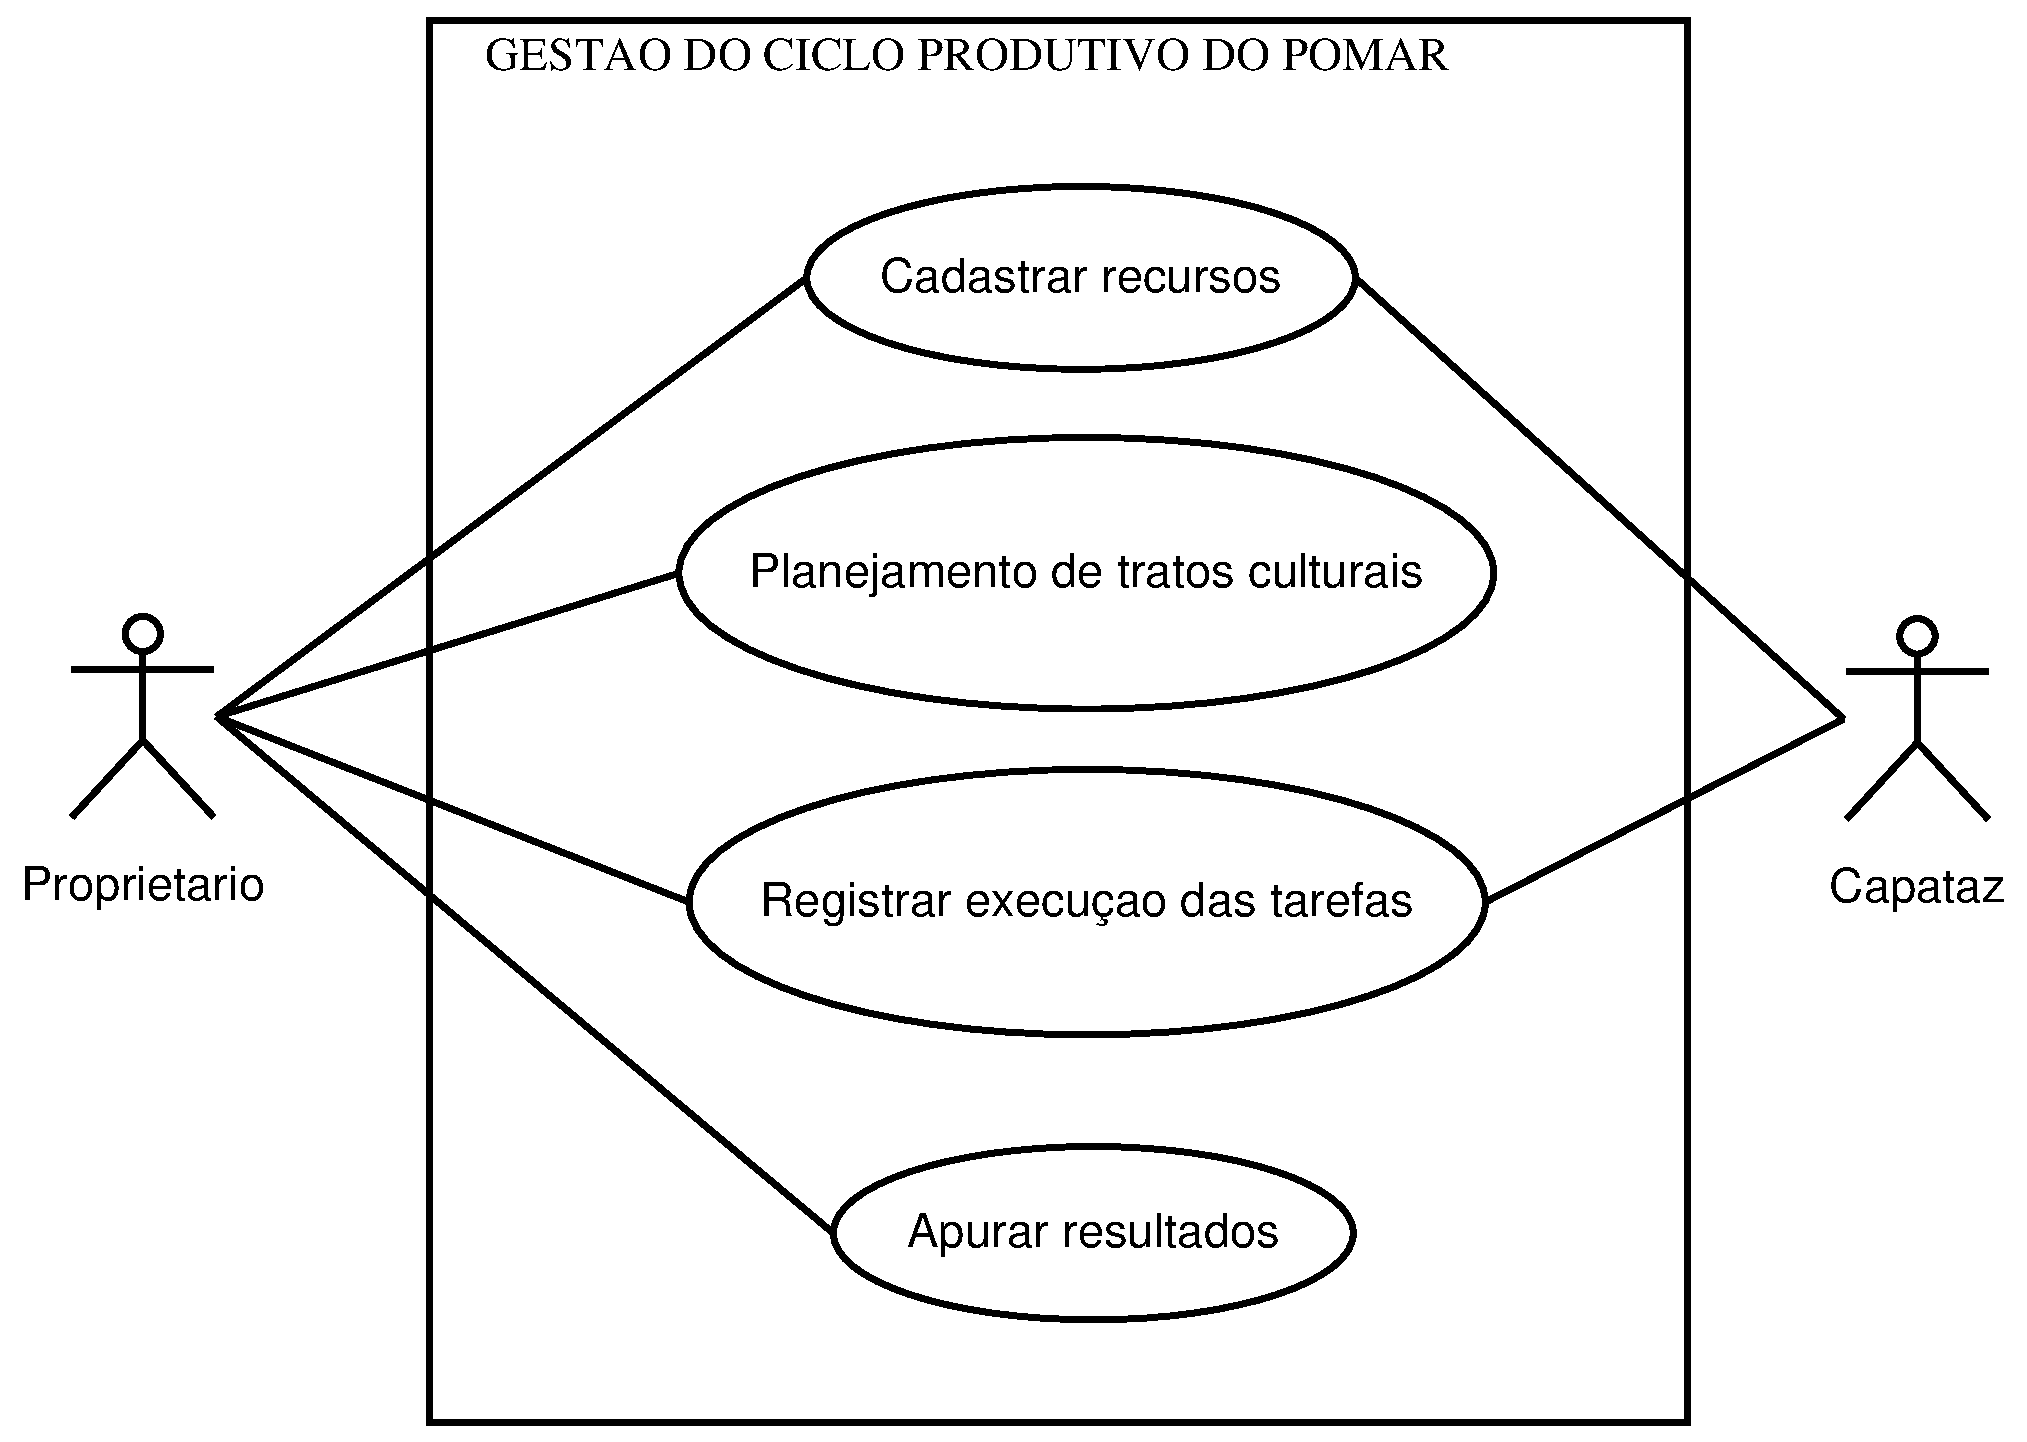
\includegraphics{diagramas/casodeuso.eps}} \par}
\caption{Caso de uso de neg�cios da aplica��o de gest�o do ciclo produtivo para pomares de pessegueiro}
\label{fcun}
\end{figure}


\subsection{Caso de uso: Cadastrar recursos}

\paragraph{A identifica��o e classifica��o dos recursos que o pomar disp�e para 
realiza��o das tarefas � uma tarefa crucial para uma eficaz gest�o. Visto que a 
estimativa, registro e apura��o de resultados � baseada nos recursos cadastrados.}
\paragraph{Este cadastramento deve ser flex�vel o suficiente para permitir que
o usu�rio do sistema possa faz�-lo e extend�-lo, se necess�rio.}
\paragraph{Como citado anteriormente, os recursos podem ser humanos, materiais, 
naturais e financeiros.}

\subsection{Caso de uso: Planejamento de tarefas}

\paragraph{O planejamento para execu��o das tarefas tem tamanha import�ncia
na gest�o do pomar. Com o planejamento � poss�vel estimar a necessidade de 
recursos financeiros, criar um cronograma de tarefas atrav�s do
agendamento das mesmas e, ainda, racionalizar a utiliza��o de recursos.}
\paragraph{Criado o cronograma, o sistema deve confeccionar as planilhas
para acompanhamento, a campo, da execu��o das tarefas.}

\subsection{Caso de uso: Registro das tarefas executadas}

\paragraph{O registro das tarefas executas no pomar se faz necess�rio para 
possibilitar a apura��o de resultados, servir de base para estimativas 
futuras e manter um registro hist�rico dos acontecimentos. Este registro 
deve ser feito diariamente, relacionando todas tarefas que foram executadas 
em cada lote do pomar.}

\subsection{Caso de uso: Apura��o de resultados}

\paragraph{O sistema deve responder ao final do ciclo produtivo, no m�nimo, as seguintes
perguntas:}
\begin{itemize}
\item
Quanto foi gasto em transporte, empregados, encargos sociais, juros, reforma
de m�quinas e implementos?
\item
Quanto foi o total colhido por ciclo, cultivar e lote?
\item
Relat�rio de vendas da safra (para quem foi vendido, data de entrega, por qual 
valor e qual � a previs�o de recebimentos)
\item
Qual foi o resultado final por ciclo, lote e cultivar?
\end{itemize}

\section{Modelo de dom�nio da aplica��o de gest�o para pomares de pessegueiro}

\begin{quotation}
``Modelo de dom�nio descreve qualquer modelo, cujo sujeito prim�rio
seja o mundo que o sistema de computa��o est� suportando, qualquer que seja o
estado do processo de desenvolvimento em que se esteja.'' \cite{umlessencial}
\end{quotation}

\paragraph{Neste trabalho a t�cnica utilizada para gerar o modelo de dom�nio 
foi o diagrama de classes, feito a partir de uma perspectiva conceitual.
Saliento que foi utilizado uma nota��o m�nima. J� que n�o procurou-se
captar cada detalhe, este diagrama serve apenas para dar uma id�ia global
do sistema que est� sendo constru�do.}

\paragraph{Baseado na descri��o textual do cap�tulo 4 e em primitivas de 
modelagem orientada a objetos, foi desenhado o modelo de dom�nio da
aplica��o na Figura \ref{fmda}.}

\begin{figure}[!b]
{\centering \resizebox*{0.8\textwidth}{0.3\textheight}{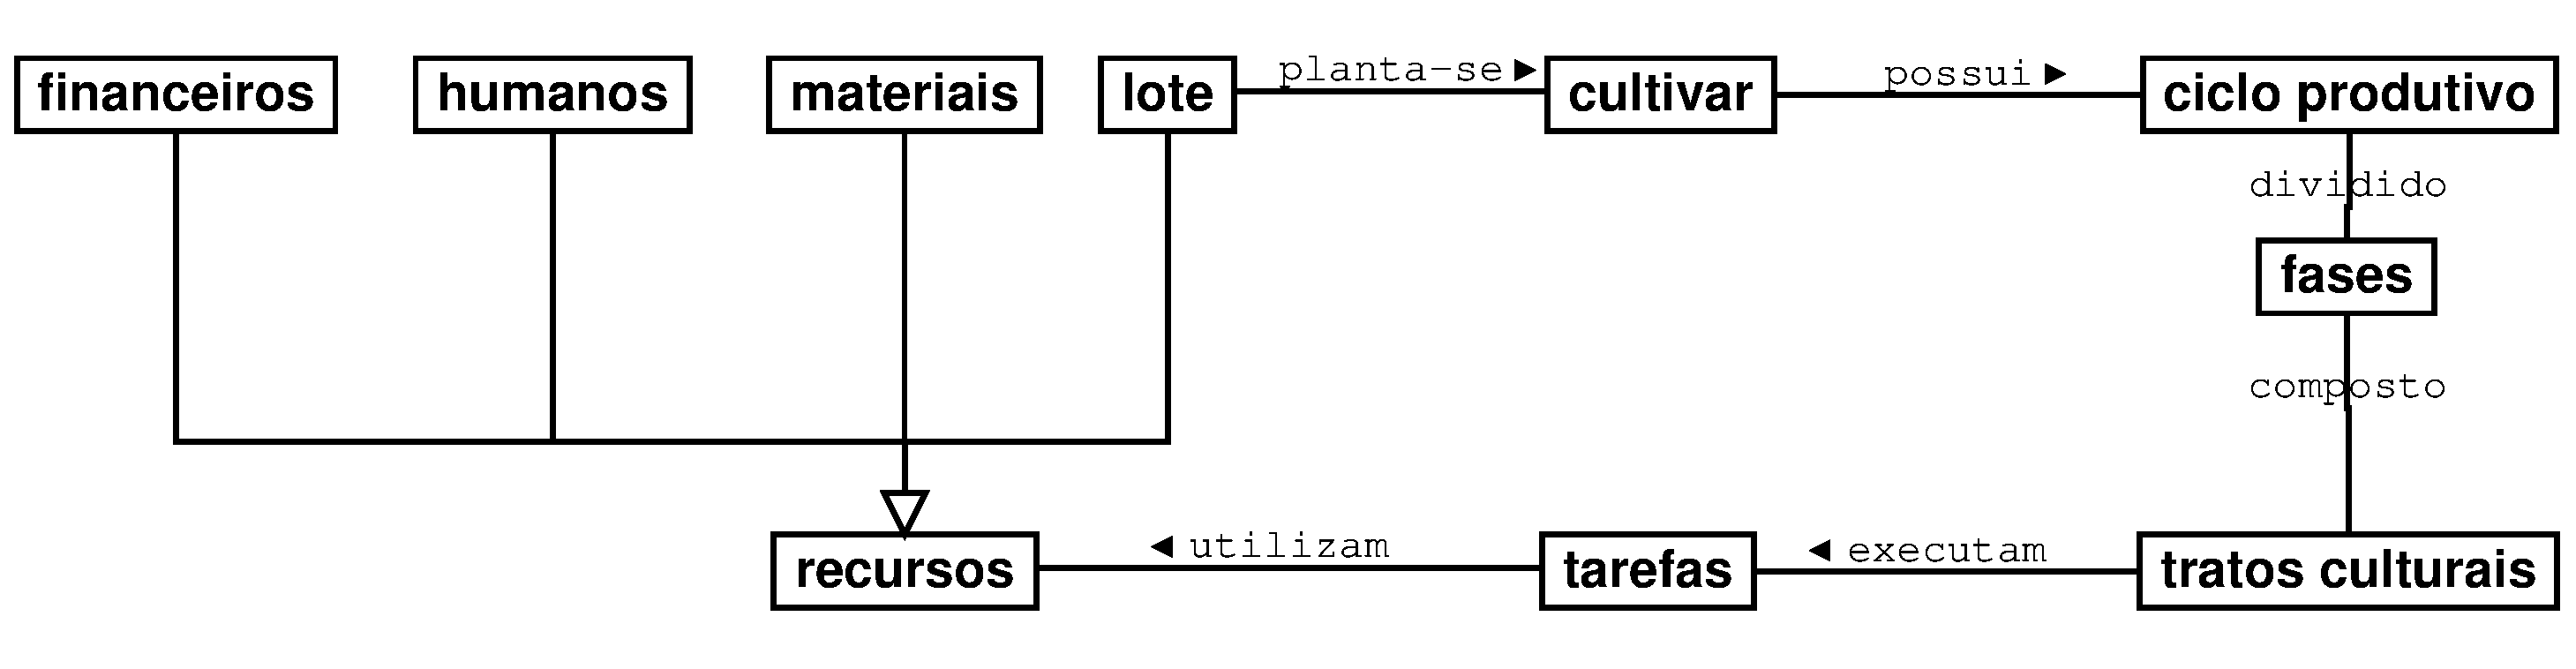
\includegraphics{diagramas/modelo_de_dominio.eps}} \par}
\caption{Modelo de dom�nio da aplica��o de gest�o para pomares de pessegueiro.}
\label{fmda}
\end{figure}

\section{Plataforma de hardware}

\paragraph{No desenvolvimento desse projeto, utilizarei a plataforma de hardware 
PC, baseada na arquitetura Intel x86, devido ao seu custo inferior comparado ao
de outras plataformas, facilidade de manuten��o/suporte, abund�ncia de software
livre e popularidade.}

\section{Plataforma de software}

\paragraph{Nesta se��o tratarei a respeito dos componentes de software
que pretendo utilizar no desenvolvimento/implementa��o deste trabalho.}
\begin{itemize}
\item Tecnologia de Sistema Operacional\\
GNU/Linux \cite{linux} me parece uma op��o acertada por possuir vasta 
documenta��o dispon�vel, ser est�vel e servir de plataforma de desenvolvimento 
para a maioria das outras ferramentas que utilizarei neste projeto. A 
distribui��o utilizada ser� Red Hat \cite{redhat} porque � a distribui��o que 
tenho mais experi�ncia.
\item Tecnologia de Banco de dados\\
PostgreSQL \cite{pgsql}, por ser o �nico banco de dados h�brido livre, 
suportando parcialmente a orienta��o a objetos.
\item Tecnologia de Servidor web\\
Apache � o servidor escolhido. Robusto, veloz, extens�vel (suporta PHP) e de 
f�cil configura��o, o tornam uma boa op��o para utiliza��o 
neste projeto.
\item Tecnologia de Gera��o din�mica de p�ginas web\\
PHP \cite{php} � a ferramenta eleita por possuir suporte a orienta��o a 
objetos, PostgreSQL, Apache e por ser desenvolvido primeiramente sobre GNU/Linux.
\item Tecnologia para Desenho de modelos\\
O software Dia \cite{dia} foi a melhor op��o encontrada, j� que suporta a 
nota��o Unified Modeling Language (UML\footnote{%
\textbf{Unified Modeling Language} � um padr�o notacional para aplica��es 
orientada a objetos.}) e � um software livre.
\end{itemize}

\section{M�o-de-obra para desenvolvimento/implementa��o deste trabalho}

\paragraph{No desenvolvimento deste trabalho estou procurando consultoria de 
pessoas que conhe�am profundamente o assunto que estou enfrentando dificuldades
de aprendizado.}
\paragraph{Na implementa��o, a princ�pio, n�o
ser� utilizado qualquer m�o-de-obra externa.}


\chapter{PROJETO}

\section{Introdu��o}

\paragraph{� nesta fase do processo de desenvolvimento que a aplica��o vai 
come�ar
a ser constru�da e implementada em fases iterativas e incrementais.}
\paragraph{Primeiramente ser�o desenhados os casos de uso de sistema da 
aplica��o,
baseado no caso de uso de neg�cio apresentado na fase de elabora��o. Feito isso, 
partirei para a execu��o das fases utilizando a OOHDM.}
\paragraph{A pr�xima se��o aborda rapidamente o m�todo de projeto que utilizarei
na constru��o deste sistema.}
\paragraph{Na se��o subseq�ente teremos o projeto da aplica��o proposta com
este trabalho.}

\section{Object-Oriented Hypermedia Design Method}

\paragraph{Como foi colocado na Se��o \ref{sec:oohdm}, a OOHDM � um m�todo de 
projeto
para aplica��es hiperm�dia que divide a constru��o do sistema em 4 atividades.}
\paragraph{A seguir, explanarei de forma resumida, cada
uma das atividades desenvolvidas em um projeto OOHDM.}

\subsection{Modelagem conceitual}

\paragraph{A modelagem conceitual compreende a primeira atividade do m�todo 
OOHDM, sendo respons�vel pela an�lise do dom�nio da aplica��o, englobando assim 
todo o universo de informa��es relevantes para a aplica��o em quest�o. \cite{patricia}}
\paragraph{Durante a modelagem conceitual � constru�do um modelo de dom�nio da aplica��o
utilizando princ�pios de modelagem orientada a objetos. A OOHDM n�o prescreve
nenhuma nota��o em particular para produzir este esquema conceitual, podendo
ser empregado UML, OMT, OOSE ou qualquer outra. Neste trabalho 
utilizarei a
UML por acreditar que, atualmente, esta linguagem de modelagem � de fato um 
padr�o notacional para modelagem de aplica��es orientada a objetos.}
\paragraph{A finalidade desta atividade � capturar a sem�ntica do dom�nio da aplica��o.
Para isso, utiliza-se formalismos de modelagem orientada a objetos como classes,
relacionamentos e casos de uso. Produz-se um esquema conceitual composto de
classes, subsistemas, relacionamentos e perspectivas de atributos baseados em
mecanismos como classifica��o, agrega��o, generaliza��o e especializa��o.}
\paragraph{As informa��es necess�rias para cria��o do esquema conceitual foram
extra�das dos casos de uso definidos na se��o anterior. Para facilitar a
tarefa de mapeamento de casos de uso para o esquema conceitual, existe uma
ferramenta chamada User Interaction Diagram (UID) que descreve a troca de 
informa��es entre o sistema e o usu�rio em um alto n�vel de abstra��o. Maiores
informa��es sobre UID s�o descritas em \cite{UID}.}
\paragraph{Devido a restri��o de tempo para desenvolvimento deste trabalho,
n�o foi poss�vel aplicar a ferramenta de UID nos casos de uso desta aplica��o,
sendo que o mapeamento se deu de maneira emp�rica e intuitiva.}

\subsection{Projeto navegacional}

\paragraph{Segundo \cite{ROS96} ``Os aplicativos de hiperm�dia s�o projetados 
para efetuar navega��o atrav�s de um espa�o de informa��es''.}
\paragraph{Em OOHDM, uma aplica��o � vista como um conjunto de vis�es 
navegacionais \textbf{derivadas} do modelo conceitual constru�do na atividade 
anterior. ``Esta � uma das maiores inova��es da OOHDM, j� que reconhece objetos 
que o usu�rio navega \textbf{n�o} como objetos conceituais, mas sim, outros 
tipos de objetos que s�o ``constru�dos'' de um ou mais objetos conceituais'' 
\cite{DHAUO}. Logo, o modelo conceitual funcionar� como um reposit�rio 
compartilhado de modelagem, a partir do qual construiremos diferentes vis�es 
navegacionais do dom�nio do problema, baseado nos usu�rios que utilizar�o a 
aplica��o e as tarefas que realizar�o nele \cite{ROS96}.}
\begin{quotation}
``Cada vis�o define um conjunto de contextos e classes navegacionais. Os contextos
navegacionais expressam a estrutura navegacional geral do aplicativo hiperm�dia,
enquanto as classes navegacionais, como os n�s e os elos, especificam os objetos
que ser�o vistos pelo usu�rio.

Os n�s representam `janelas' l�gicas em classes definidas no esquema conceitual
atrav�s de uma mapeamento que fornece um `corte e colagem' de atributos conceituais
semelhantes �s vis�es dos objetos.

Os contextos navegacionais s�o um conjunto de n�s, elos e outros contextos navegacionais
(aninhados) que auxiliam na organiza��o dos objetos navegacionais, fornecendo
espa�os de navega��o consistentes e, deste modo, diminuindo as chances do usu�rio
`perder-se no hiperespa�o''' \cite{ROS96}.
\end{quotation}

\subsubsection{O esquema de classes navegacionais da aplica��o}

\begin{quotation}
``Um dos produtos da atividade de projeto de navega��o � o esquema navegacional,
constru�do sobre n�s e elos. As classes navegacionais definidas nesta atividade
s�o especificadas como especializa��es de um conjunto de classes b�sicas que
definem a sem�ntica dos objetos navegacionais'' \cite{ROS96}.
\end{quotation}

\paragraph{Em OOHDM h� um conjunto de tipos pr�-definidos de classes navegacionais como:
n�s, links, �ncoras e estruturas de acesso. A sem�ntica dos n�s, links e �ncoras
s�o as mesmas utilizadas em aplica��es hiperm�dia usuais, enquanto que estruturas
de acesso representam as poss�veis maneiras de acessar n�s.}

\subsubsection{O diagrama de contextos}

\begin{quotation}
``Um contexto de navega��o � um conjunto de objetos (n�s, elos e, recursivamente,
outros contextos navegacionais) que est�o relacionados de acordo com algum 
aspecto (ex.: os n�s do mesmo tipo que apresentam um atributo com o mesmo
conte�do; os n�s do mesmo tipo que apresentam um relacionamento com um mesmo
n� de outro tipo; os n�s de tipos diferentes que apresentam uma caracter�stica
em comum).'' \cite{patricia}
\end{quotation}

\paragraph{Os contextos de navega��o da aplica��o ficam documentados em cart�es
pr�prios e s�o representados graficamente no diagrama de contextos.}

\paragraph{Os contextos possuem formas pr�-definidas de acesso e de navega��o
entre seus elementos, bem como restri��es de acesso a usu�rios.}

\paragraph{H� um tipo de contexto de navega��o chamado \textbf{estrutura de 
acesso} que age como �ndice para outros contextos. Em cada estrutura de acesso
s�o especificados atributos ``seletores'', que s�o os objetos que ativam a 
navega��o a outros contextos.}

\subsubsection{Classes em contexto}

\paragraph{Classes em contexto s�o artif�cios utilizados para acrescentar
caracter�sticas a n�s conforme o contexto em que est�o sendo acessados. Estas
classes em contexto s� se fazem necess�rias caso o n� deva possuir uma apar�ncia 
diferente e �ncoras distintas no contexto em quest�o.}
\paragraph{Quando um n� possui atributos com m�ltiplas perspectivas, � um ind�cio
para utiliza��o de classes em contexto.}
\paragraph{Na representa��o de classes em contexto utiliza-se a mesma nota��o
de classes da UML, diferenciando-se apenas pela adi��o de 
um compartimento onde � especificado os
contextos nos quais a classe em contexto participa.}

\subsection{Projeto de interface abstrata}

\paragraph{A atividade de Projeto de Interface Abstrata compreende uma 
abordagem para especificar a interface de usu�rio para aplica��es
hiperm�dia. Esta atividade deve ser desenvolvida antes de iniciar a 
atividade de implementa��o, de forma que seja independente do ambiente onde
se pretende efetivamente construir o aplicativo, sempre procurando manter uma
coer�ncia com o ambiente de implementa��o (por exemplo, de nada adianta 
especificar algo que o ambiente de implementa��o n�o suporta).}
\paragraph{Na especifica��o da interface abstrata utilizamos o conceito de 
Abstract Data Views (ADVs). ADVs s�o objetos que especificam a organiza��o
e procedimentos da interface, s�o abstratos porque sua real apar�ncia f�sica
� feita na fase de implementa��o. ADVs possuem um estado e uma 
interface, onde a interface � utilizada para entrada e/ou sa�da de eventos
externos gerados pelo usu�rio.}
\paragraph{OOHDM tamb�m utiliza Abstract Data Objects (ADOs), que similarmente
aos ADVs s�o objetos, s� que n�o suportam eventos externos gerados pelo usu�rio.}
\begin{quotation}
``Em uma t�pica aplica��o utilizando ADVs, temos um conjunto de ADOs
gerenciando estruturas de dados e de controle, e um conjunto de objetos
de interface (inst�ncias de ADVs) gerenciando aspectos de interface da aplica��o, 
como entrada de dados do usu�rio e sa�da de dados do sistema para o usu�rio.'' \cite{IWHD}
\end{quotation}
\paragraph{``No contexto da OOHDM, os objetos navegacionais (n�s, elos, classes 
em contexto e estruturas de acesso) agir�o como ADOs e estar�o associados a ADVs
que ser�o usados para especificar a sua apar�ncia para o usu�rio.'' \cite{IWHD}}
\paragraph{Utilizamos tamb�m uma vari�vel chamada ``ContextoPerceptivo'' para
indicar os objetos que s�o percept�veis num dado momento. Todo e qualquer objeto
que vier a se tornar vis�vel � acrescido a ``ContextoPerceptivo'', enquanto
que todos aqueles que forem exclu�dos da vari�vel deixam de ser percept�veis.}

\subsubsection{Diagramas de Configura��o}

\paragraph{Nesta fase constr�i-se Diagramas de Configura��o, que s�o utilizados
para representar os relacionamentos entre os objetos de interface e os objetos
navegacionais. \cite{patricia}}
\paragraph{Al�m de representarem os objetos de interface (ADVs), os diagramas de
configura��o especificam outras caracter�sticas da interface abstrata da aplica��o,
que conforme \cite{patricia} s�o:}
\begin{itemize}
\item os eventos externos iniciados pelo usu�rio e que ser�o manipulados pelos ADVs;
\item os relacionamentos estruturais entre os ADVs;
\item os relacionamentos entre os ADVs (que representam os objetos de interface)
e os ADOs (que representam os objetos navegacionais).
\end{itemize}

\subsubsection{ADVcharts\label{sec:advcharts}}

\paragraph{Outro diagrama tamb�m � constru�do nesta fase, os ADVcharts. Estes 
procuram apresentar as transforma��es ocorridas nos ADVs,
sendo que cada ADVchart est� relacionado com uma tela da interface.}
\paragraph{Enquanto que os Diagramas de Configura��o representam a estrutura
est�tica da interface, utilizamos ADVcharts para representar a estrutura din�mica.}

\subsection{Implementa��o}

\paragraph{A atividade de Implementa��o � a �ltima etapa de uma itera��o em OOHDM,
sendo que agora � o momento de transformarmos os artefatos abstratos produzidos nas
fases anteriores em artefatos concretos de software.}
\paragraph{Para feitura deste mapeamento utilizaria-se ferramentas que suportassem 
a nota��o OOHDM, bem como um framework\footnote{%
Segundo \cite{pizzol} ``um \textbf{framework} � o esqueleto de uma aplica��o
que pode ser customizada por um desenvolvedor de aplica��o''.}
que possibilitasse a implementa��o de uma 
especifica��o OOHDM da maneira menos traum�tica poss�vel.}
\paragraph{Infelizmente n�o h� ferramentas para desenho dos diagramas, fazendo
necess�rio a adapta��o das ferramentas existentes a nota��o da metodologia.}
\paragraph{Quanto aos frameworks, existem atualmente duas op��es que abordo
brevemente a seguir.}

\begin{itemize}
\item \textbf{OOHDM-Java}\\
\cite{pizzol} prop�e um framework em Java para implementa��o na WWW 
de aplica��es hiperm�dia modeladas com OOHDM.\\
O framework � implementado com uma biblioteca de classes em Java,
que representa as primitivas OOHDM na web.\\
OOHDM-Java � considerado um framework caixa-branca \footnote{``Um framework
� considerado \textbf{caixa-branca} quando � necess�rio que programadores
estendam o seu projeto e sua implementa��o, pelo menos at� um certo grau
de detalhe, para utiliz�-lo. Por esta raz�o, esses tipos de frameworks
geralmente s�o mais dif�ceis de aprender e usar.'' \cite{pizzol}}
, sendo portanto,
de dif�cil aprendizado. Infelizmente, n�o h� tempo para estudar todo o
framework e ainda implementar um prot�tipo.\\
Apesar dos requisitos de sistema especificados na disserta��o
relacionarem apenas software propriet�rio, acredito que seja poss�vel obter
plataforma igual baseada em software livre.
\item \textbf{OOHDM-WEB}\\
\cite{isabela} prop�e um ambiente de desenvolvimento para dar
suporte �s aplica��es WWW modeladas com OOHDM. Esse ambiente faz uso da
linguagem script CGILua e o pacote DBLua (para acesso a bases de dados)
e permite a implementa��o de script CGI, que geram p�ginas dinamicamente,
baseando-se em templates pr�-definidos e nos dados contidos em um
banco de dados.\\
Uma caracter�stica interessante deste ambiente � a 
possibilidade de compila��o, gerando uma aplica��o est�tica,
eliminando desta maneira a necessidade de manter um banco de dados e o 
``overhead'' causado pela gera��o din�mica das p�ginas.\\
Infelizmente n�o h� implementa��o deste ambiente de 
desenvolvimento para rodar sobre software livre.
\end{itemize}

\paragraph{Acredito ser esta a atividade mais delicada da OOHDM na atualidade,
a falta de um framework para implementa��o faz o desenvolvedor pensar duas
vezes antes de utilizar um m�todo, porque � sabido que todo o trabalho feito
nas atividades anteriores n�o � mapeado de forma direta para artefatos
concretos de software.}
\paragraph{Como n�o existe um framework para PHP, decidi criar um para poder
implementar o prot�tipo deste trabalho.}


\section{Casos de uso de sistema}

\paragraph{Nesta se��o vamos refinar os casos de uso de neg�cio propostos
na fase anterior em casos de uso de sistema.}

\section{A constru��o do caso de uso ``Cadastrar recursos''}
\paragraph{Nesta se��o ser� constru�do o caso de uso ``Cadastrar
recursos'', sendo que este caso de uso � utilizado tanto pelo propriet�rio
como pelo capataz do pomar. Na Figura \ref{fcr} procurei diagramar o caso de uso
proposto nesta se��o.}

\begin{figure}[h]
{\centering \resizebox*{0.9\textwidth}{0.2\textheight}{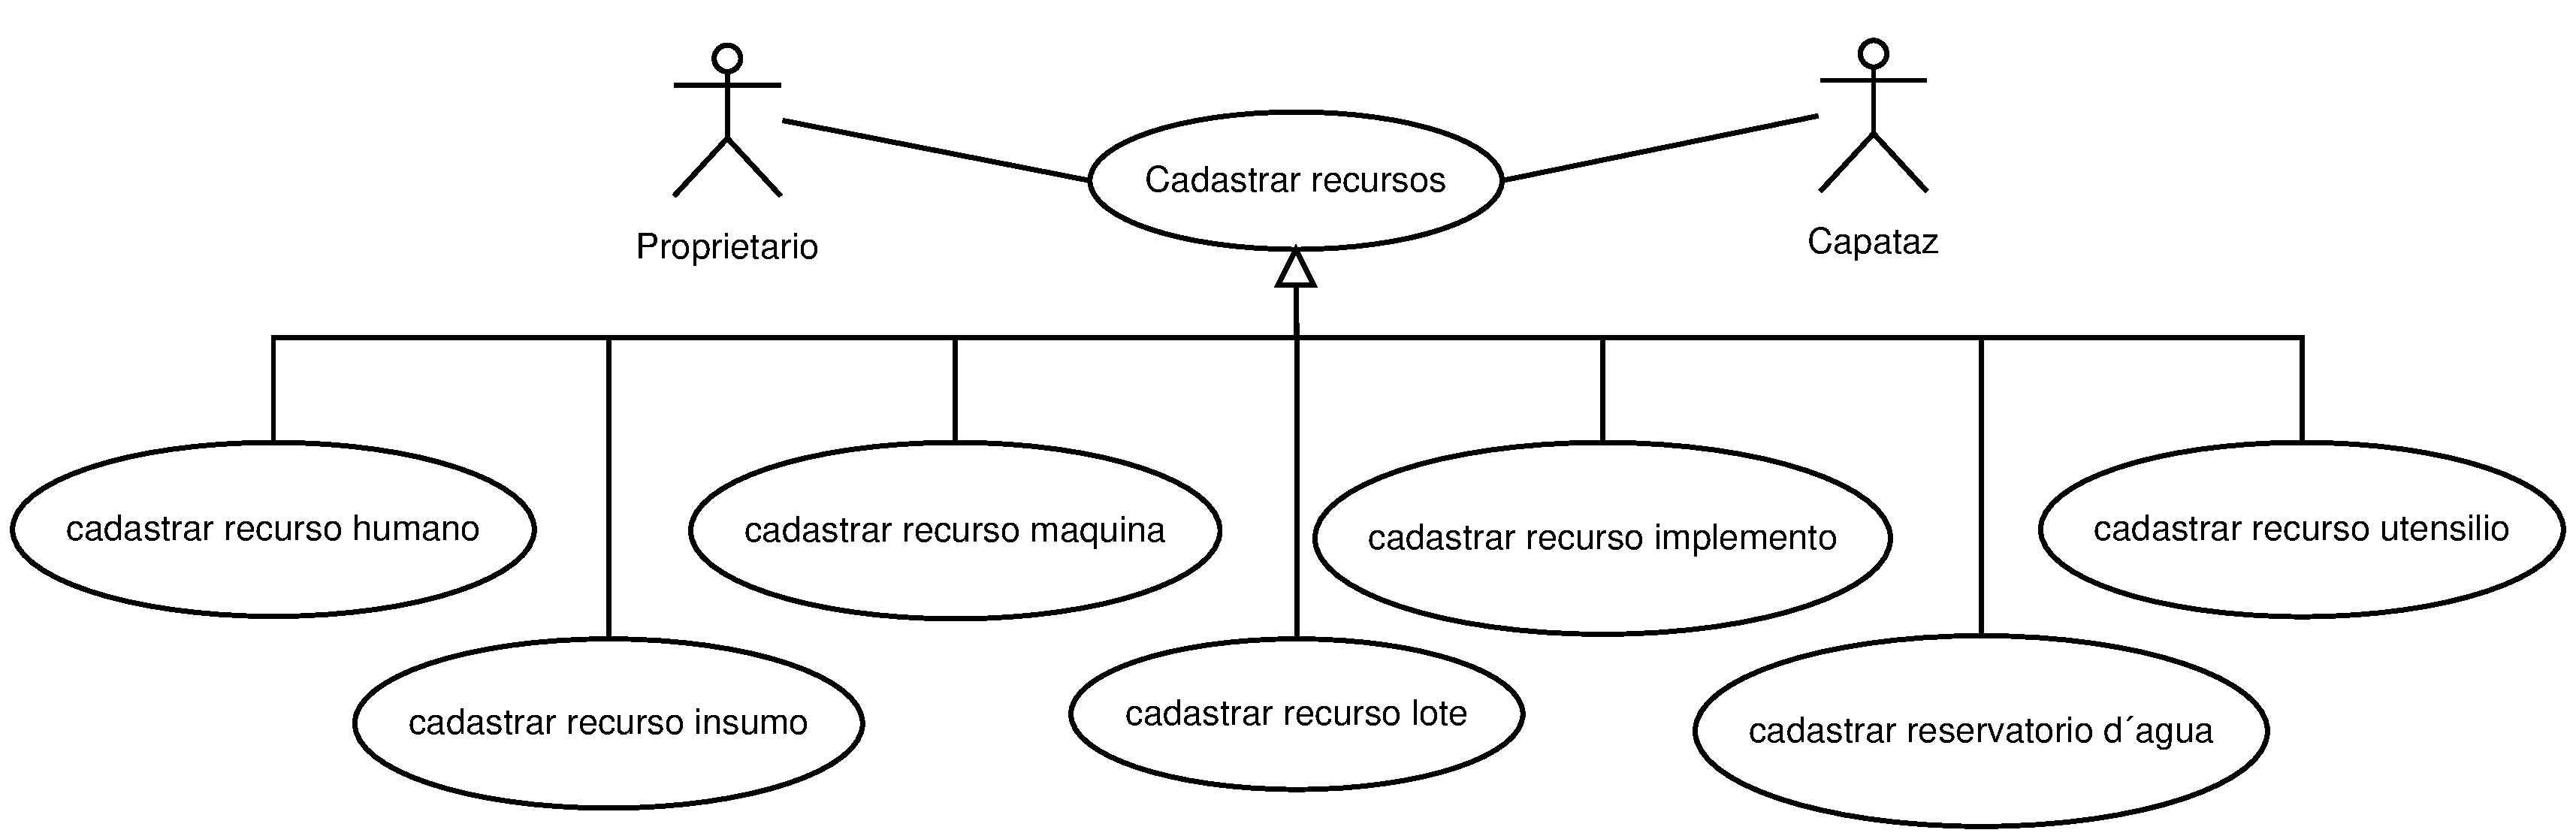
\includegraphics{diagramas/casodeusocadastrarrecursos.eps}} \par}
\caption{Caso de uso de ``Cadastrar recursos''}
\label{fcr}
\end{figure}

\paragraph{Os ``casos de uso de sistema'' (confesso que a especifica��o mais 
parece um dicion�rio de dados do que a formaliza��o de casos de uso) est�o 
textualizados abaixo:}

\begin{itemize}

\item \textbf{Cadastrar Recursos Humanos}\\
O cadastro da m�o-de-obra empregada no pomar, deve ser feita cadastrando dados
como:
\begin{itemize}
\item Nome completo do empregado
\item Apelido
\item CPF
\item RG
\item Estado civil
\item Sexo
\item Forma de Pagamento (diarista, mensalista, empreiteiro, horista)
\item Sal�rio
\item Dependentes (grau de depend�ncia, nome e data de nascimento)
\item Observa��es (data, coment�rio)
\end{itemize}

\item \textbf{Cadastrar Recursos M�quinas}\\
O cadastro de recursos materiais da classe m�quinas agr�colas, compreende os 
aparelhos capazes de produzir energia que pode ser
utilizada na execu��o de tarefas agr�colas.\\
Ex.: trator, moto-serra,
motor estacion�rio (el�trico ou a combust�o), etc.\\
O cadastro desses aparelhos deve conter dados como:
\begin{itemize}
	\item C�digo
	\item Fabricante
	\item Modelo
	\item N�mero de S�rie
	\item Cor
	\item N�mero do Chassi
	\item Ano de Fabrica��o
	\item Classe
	\begin{itemize}
		\item Trator
		\item Moto-serra
		\item motor estacion�rio
	\end{itemize}
\end{itemize}

\item \textbf{Cadastrar Recursos Implementos}\\
Todos aqueles aparelhos que acoplados a uma m�quina s�o capazes de
executar tarefas agr�colas devem ser cadastrados como recursos materiais da
classe implemento.\\
Ex.: pulverizador, semeadeira, arado, carreta, etc.\\
Desses implementos s�o armazenados os seguintes dados:
\begin{itemize}
	\item C�digo
	\item Marca
	\item Ano de Fabrica��o
	\item N�mero de F�brica
	\item Classe
	\begin{itemize}
		\item grade
		\begin{itemize}
			\item n�mero de discos
		\end{itemize}
		\item arado
		\begin{itemize}
			\item n�mero de discos
		\end{itemize}
		\item semeadeira
		\begin{itemize}
			\item forma de distribui��o: a lan�o, 2, 3, 4, 5, 20 linhas, etc.
		\end{itemize}
		\item pulverizador
		\begin{itemize}
			\item turbina, barra, pistola, etc.
		\end{itemize}
		\item carreta
		\begin{itemize}
			\item n�mero de rodas
			\item capacidade (em toneladas)
		\end{itemize}
	\end{itemize}
\end{itemize}

\item \textbf{Cadastrar Recursos Insumos}\\
Os insumos compreendem aqueles produtos que se usa no desenvolver de um trato 
cultural no per�odo de uma safra.\\
Ex.: fungicidas, inseticidas, adubo, etc.\\
Os seguintes dados fazem parte do cadastro de insumos:
\begin{itemize}
	\item C�digo
	\item Nome do Produto
	\item Tipo
	\begin{itemize}
		\item Fungicida
		\item Inseticida
		\item Herbicida
		\item Adubo (F�rmula)
	\end{itemize}
	\item Fabricante
	\item Unidade
\end{itemize}

\item \textbf{Cadastrar Recursos Utens�lios}\\
O cadastro dos recursos materiais da classe utens�lios se d� relacionando 
todas pequenas ferramentas manuais utilizadas na execu��o de tarefas
no pomar.\\
Ex.: tesouras, serrotes, pulverizadores costal, enxada, etc.\\
Os seguintes dados fazem parte do cadastro de utens�lios:
\begin{itemize}
\item Nome do Utens�lio
\item Marca
\item Modelo
\item Classe (tesoura de poda, serrote de poda, serrote comum, enxada, etc)
\end{itemize}

\item \textbf{Cadastrar Recurso Lote}\\
O cadastro dos lotes � feito agrupado os talh�es ou lavouras por cultivar e 
�poca de implanta��o.\\
Para cadastro dos lotes considera-se os seguintes dados:
\begin{itemize}
\item �rea (em hectares)
\item N�mero de plantas
\item Localiza��o
\item Cultivar
\end{itemize}

\item \textbf{Cadastrar Recurso Reservat�rio d'�gua}\\
Dos reservat�rios d'�gua instalados no pomar, cadastra-se os seguintes dados.
\begin{itemize}
\item Localiza��o
\item Capacidade (em \( m^{3} \))
\item Classe
	\begin{itemize}
	\item A�ude
	\item Barragem
	\item Tanque
	\item Po�o Artesiano
	\end{itemize}
\end{itemize}
%\item \textbf{Cadastrar recursos cultivar}\\
%Neste cadastro relaciona-se os cultivares que s�o/ser�o utilizados no pomar. 
%Ex.: �gata, diamante, precocinho, etc.\\
%Para cadastro dos cultivares, deve-se considerar os seguintes dados:
%\begin{itemize}
%\item Nome
%\item Origem hist�rica
%\item Descri��o da Planta
%\item Descri��o do Fruto
%\item Observa��es
%\item Fotografia
%\end{itemize}

\end{itemize}

\subsection{Modelagem conceitual}

\paragraph{O esquema conceitual do caso de uso de neg�cio ``Cadastrar recursos''
est� representado na Figura \ref{feccr}.}

\begin{figure}[!h]
{\centering \resizebox*{\textwidth}{0.9\textheight}{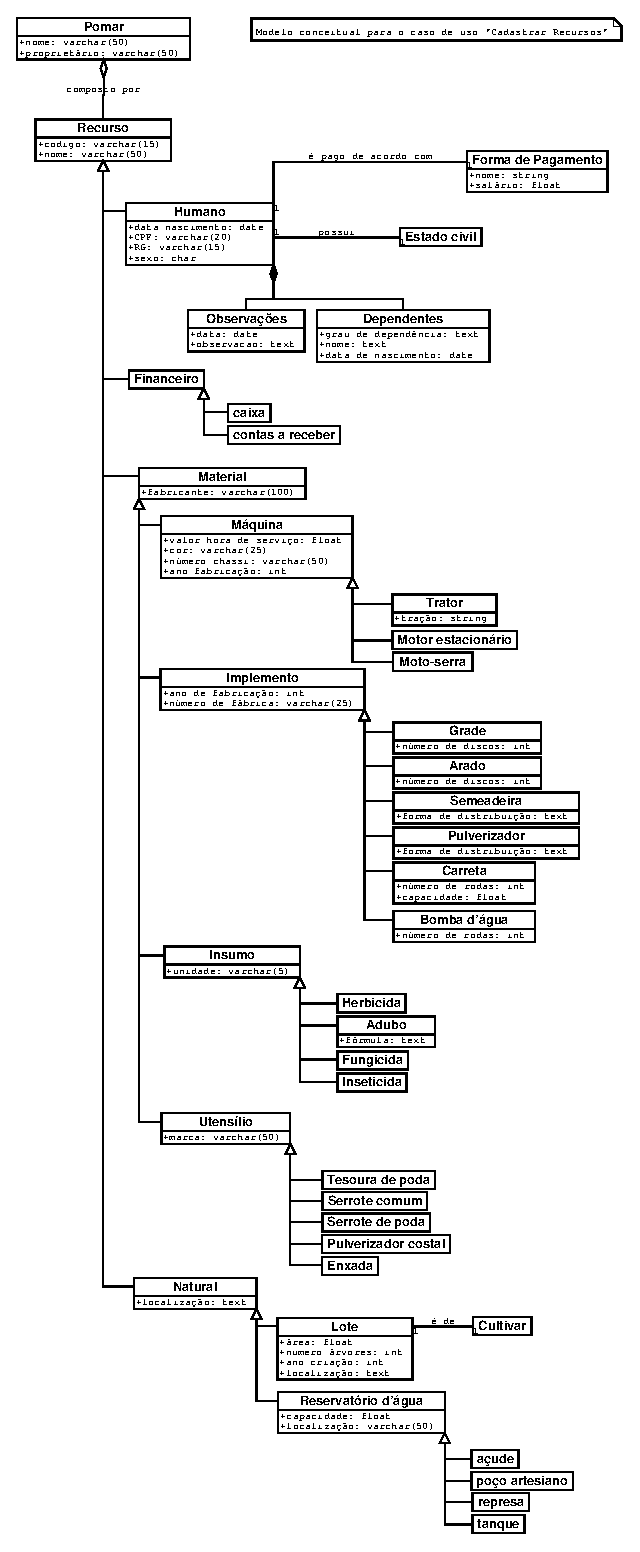
\includegraphics{diagramas/cad_rec_modelo_conceitual.eps}} \par}
\caption{Esquema conceitual do caso de uso de ``Cadastrar recursos''}
\label{feccr}
\end{figure}

\subsection{Projeto navegacional}

\paragraph{O produto da atividade de projeto navegacional do caso de uso 
``Cadastrar recursos'' est� documentado atrav�s de seu esquema navegacional
(Figura \ref{fencr}) e diagrama de contextos (Figura \ref{fdccr}).}

\begin{figure}[!h]
{\centering \resizebox*{\textwidth}{0.9\textheight}{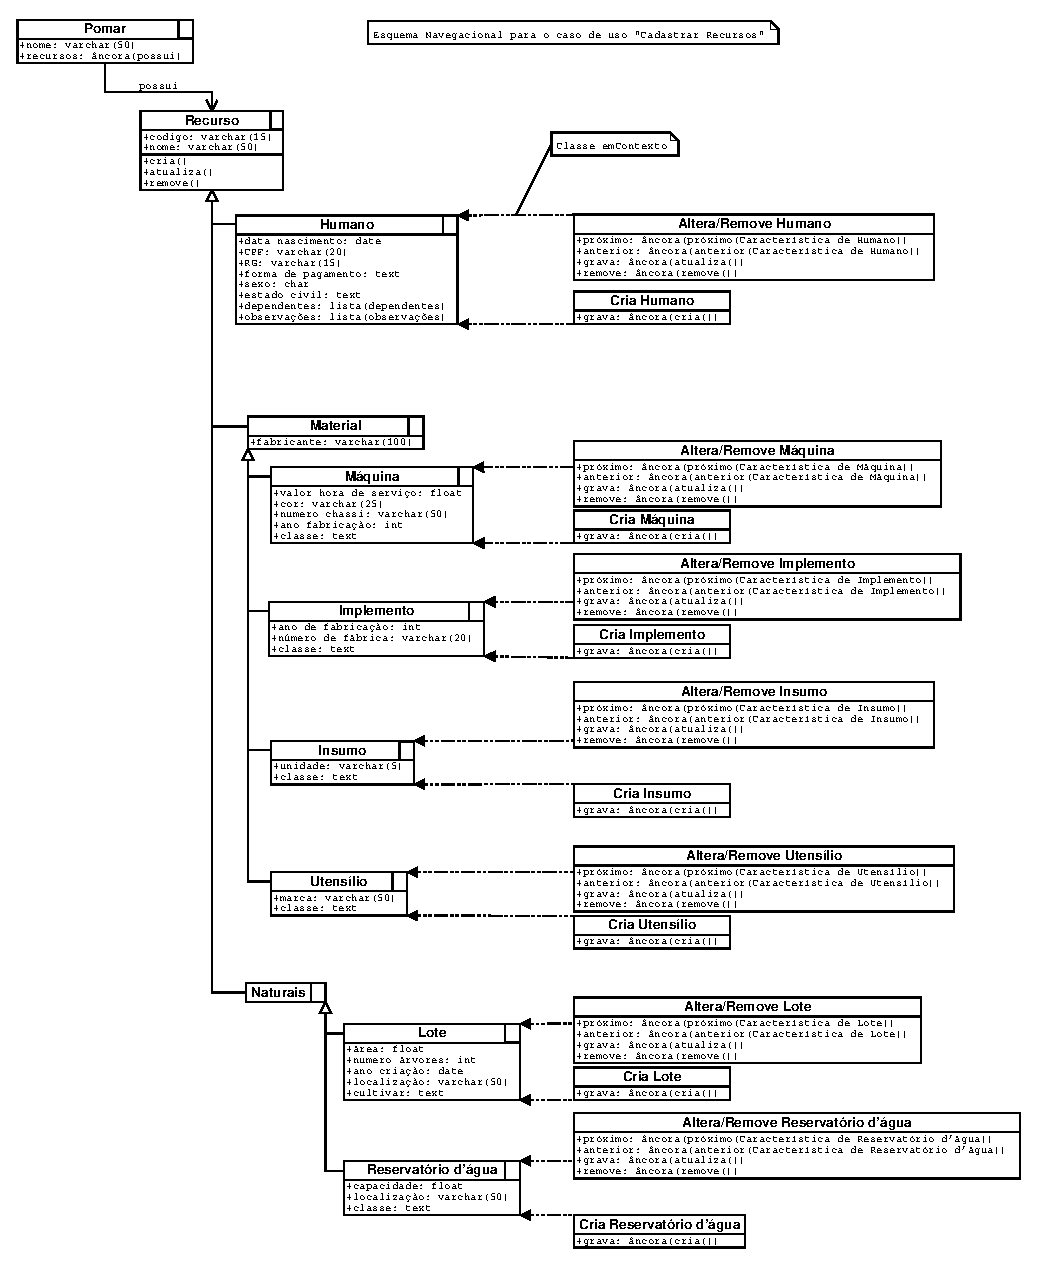
\includegraphics{diagramas/cad_rec_esquema_navegacional.eps}} \par}
\caption{Esquema navegacional do caso de uso de ``Cadastrar recursos''}
\label{fencr}
\end{figure}

\begin{figure}[!h]
{\centering \resizebox*{\textwidth}{0.9\textheight}{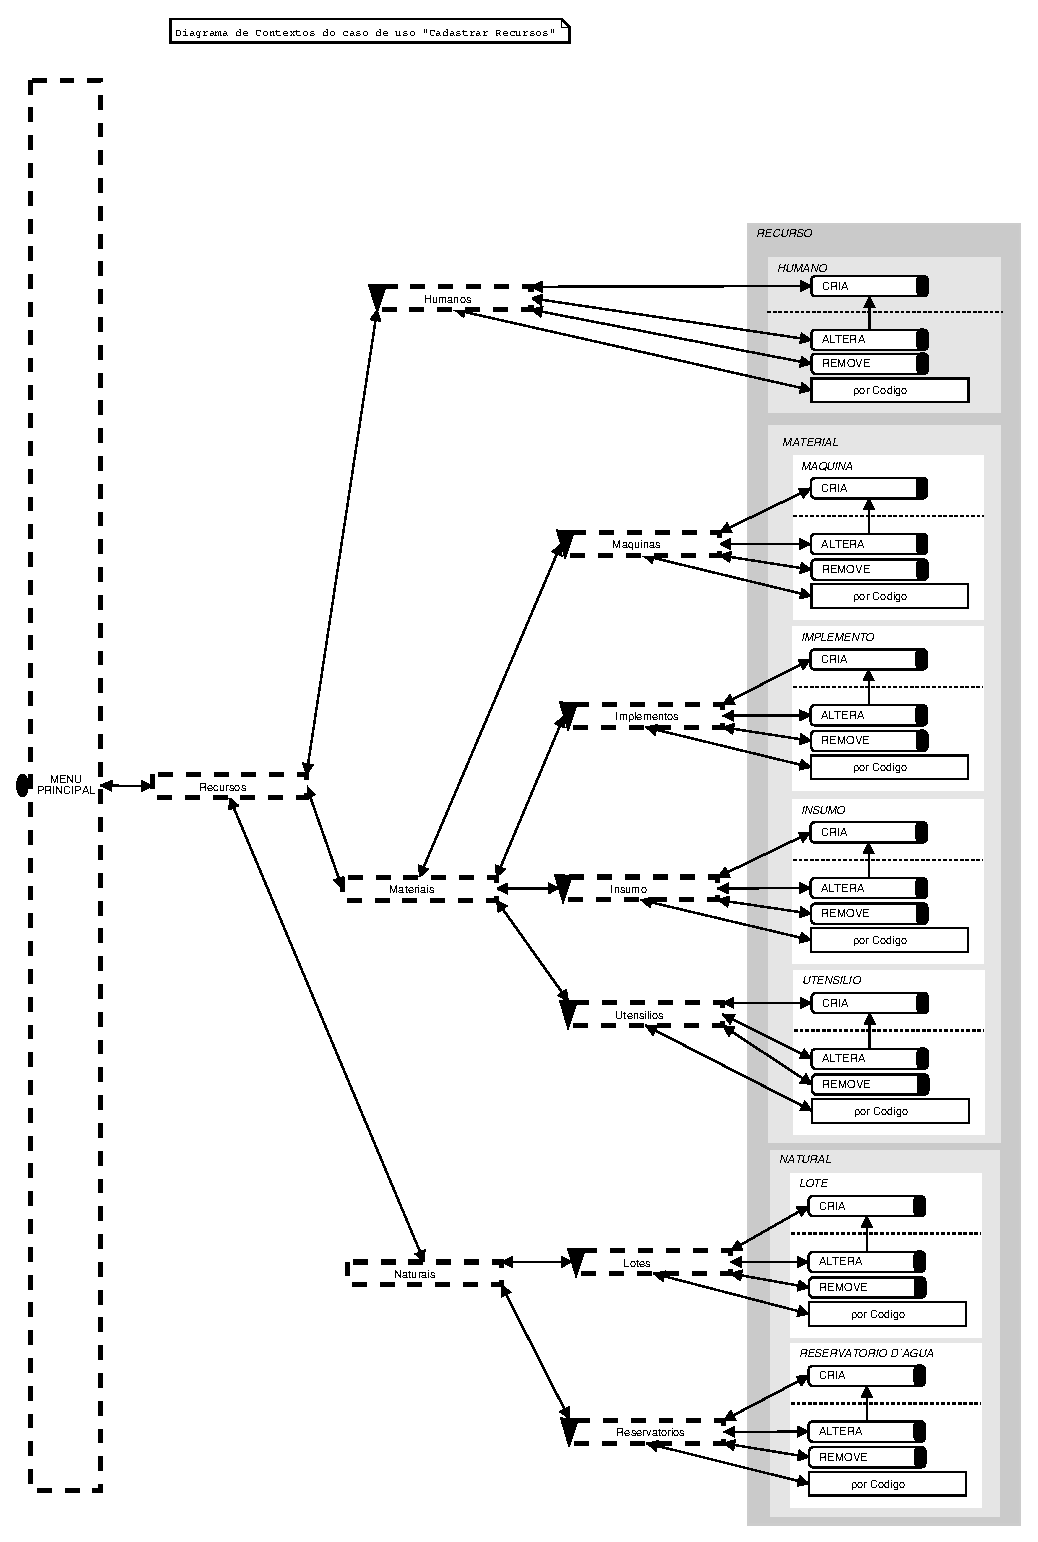
\includegraphics{diagramas/cad_rec_diag_contextos.eps}} \par}
\caption{Diagrama de Contextos do caso de uso de ``Cadastrar recursos''}
\label{fdccr}
\end{figure}

\subsection{Projeto de interface abstrata}

\paragraph{A defini��o dos ADVs principais da aplica��o, bem como, os ADVs do 
caso de uso em estudo est�o representados na Figura \ref{fadvcr}.}
\paragraph{Conv�m lembrar que alguns ADVs foram omitidos, dado que pretendo
ilustrar com a Figura \ref{fadvcr} a forma como � criado os ADVs e n�o especificar
todas possibilidades.}

\begin{figure}[!h]
{\centering \resizebox*{\textwidth}{0.9\textheight}{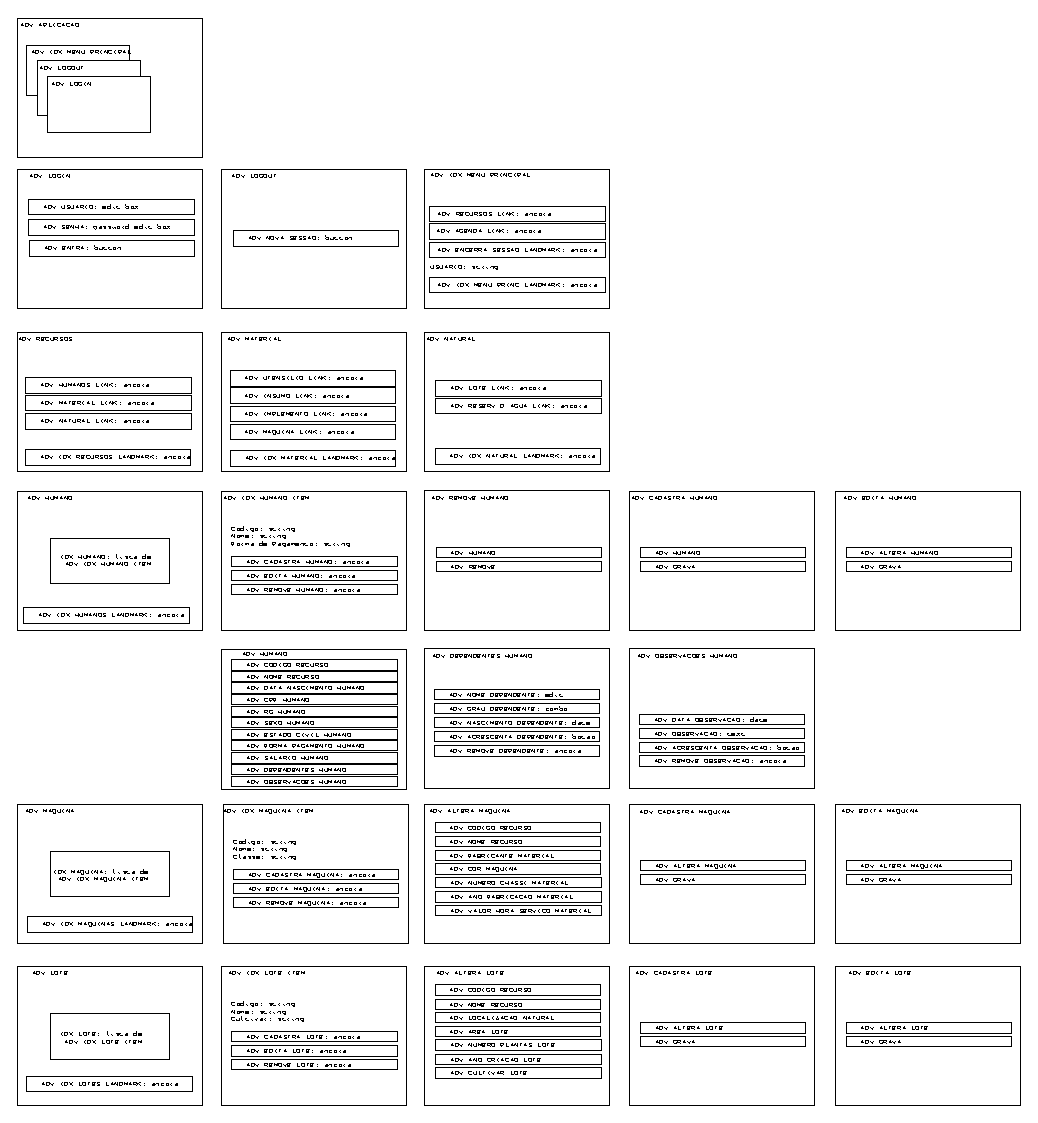
\includegraphics{diagramas/cad_rec_adv.eps}} \par}
\caption{Abstract Data Views do caso de uso ``Cadastrar recursos''}
\label{fadvcr}
\end{figure}

\subsection{Implementa��o}

\paragraph{Neste trabalho implementarei um prot�tipo do cadastro de recursos
humanos deste caso de uso, devido a restri��o de tempo.}
\paragraph{A plataforma de software utilizada foi:}
\begin{itemize}
\item Distribui��o Red Hat Linux 6.2
\item PostgreSQL 7.0.2
\item PHP 4.0.1pl3
\item Navegador Mozilla M18
\end{itemize}
\paragraph{A plataforma de hardware utilizada no desenvolvimento foi:}
\begin{itemize}
\item Processador: AMD K6-II 333 Mhz
\item Mem�ria RAM: 128 Mb
\item HD: Maxtor 91303D (13Gb) e QUANTUM FIREBALLlct10 (10Gb)
\item Drive CD-ROM: Hewlett-Packard CD-Writer Plus 8100
\item Modem: USRobotics Sportster Voice 33.6 External
\item Placa de V�deo: Diamond Stealth 6400 2 Mb (Chipset S3) 
\item Monitor de V�deo: LG Studioworks 550M
\end{itemize}

\paragraph{O diagrama de classes produzido na atividade de Modelagem Conceitual
foi traduzido para cl�usulas SQL. J� que o PostgreSQL possui heran�a, utilizei
esse recurso quando necess�rio. As rela��es entre classes foram mapeadas para 
campos que cont�m o Object Identification Number (OID\footnote{%
\textbf{Object Identification Number}: 
conforme \cite{livropgsql} cada registro no banco de dados PostgreSQL recebe 
um identificador �nico chamado OID.}) do objeto ao qual se relaciona. Maiores
informa��es sobre como mapear o esquema conceitual para uma base de dados
podem ser encontradas em \cite{patricia}.}
\paragraph{No Projeto Navegacional, o framework suporta a defini��o de
``n�s'' para a implementa��o do Esquema de Classes Navegacionais; Contextos
e Estruturas de Acesso (�ndices simples e din�micos) para implementa��o
do Esquema de Contextos Navegacionais.}
\paragraph{Classes ADV definidas no framework d�o suporte a implementa��o
do Projeto de Interface Abstrata, sendo que as met�foras de interface s�o
definidas em HTML. Apesar de n�o ter especificado \emph{ADVcharts}\footnote{%
\textbf{ADVcharts} s�o diagramas que buscam formalizar o comportamento da 
interface
da aplica��o frente a est�mulos externos (como cliques do mouse, etc.)
Maiores informa��es podem ser obtidas na se��o \ref{sec:advcharts} e
\cite{IWHD}.} neste trabalho,
foi necess�rio implementar o comportamento da interface em PHP (dentro dos
Contextos e Estruturas de Acesso) e Java Script (dentro dos ADVs).}
\paragraph{O framework n�o suporta completamente a OOHDM, at� mesmo porque
n�o � o objeto de estudo prim�rio deste trabalho. Baseado nas defini��es
encontradas em \cite{isabela} considero o framework desenvolvido como
sendo do tipo ``caixa-branca'', exigindo bom conhecimento da estrutura
interna do framework para utiliza��o do mesmo.}
\paragraph{A Figura \ref{filogin} apresenta a interface para usu�rio do
ADV LOGIN. N�o esque�a que os ADVs s�o aninhados, logo, o ADV LOGIN
est� contido no ADV APLICA��O.}

\paragraph{A Figura \ref{fimenuprincipal} apresenta a interface para usu�rio
do ADV IDX MENU PRINCIPAL.}

\begin{figure}[!h]
{\centering \resizebox*{\textwidth}{0.4\textheight}{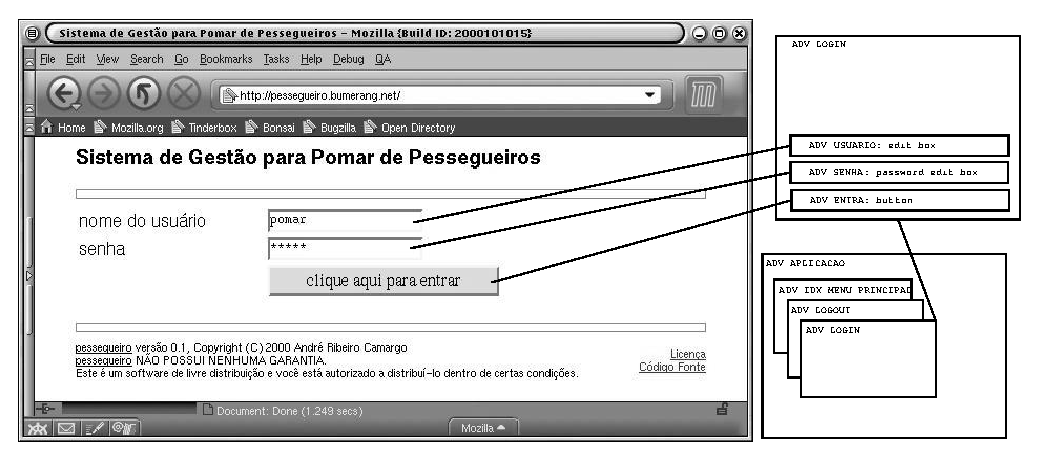
\includegraphics{diagramas/ilust_adv_login.eps}} \par}
\caption{Interface para o usu�rio do ADV LOGIN}
\label{filogin}
\end{figure}

\begin{figure}[!h]
{\centering \resizebox*{\textwidth}{0.45\textheight}{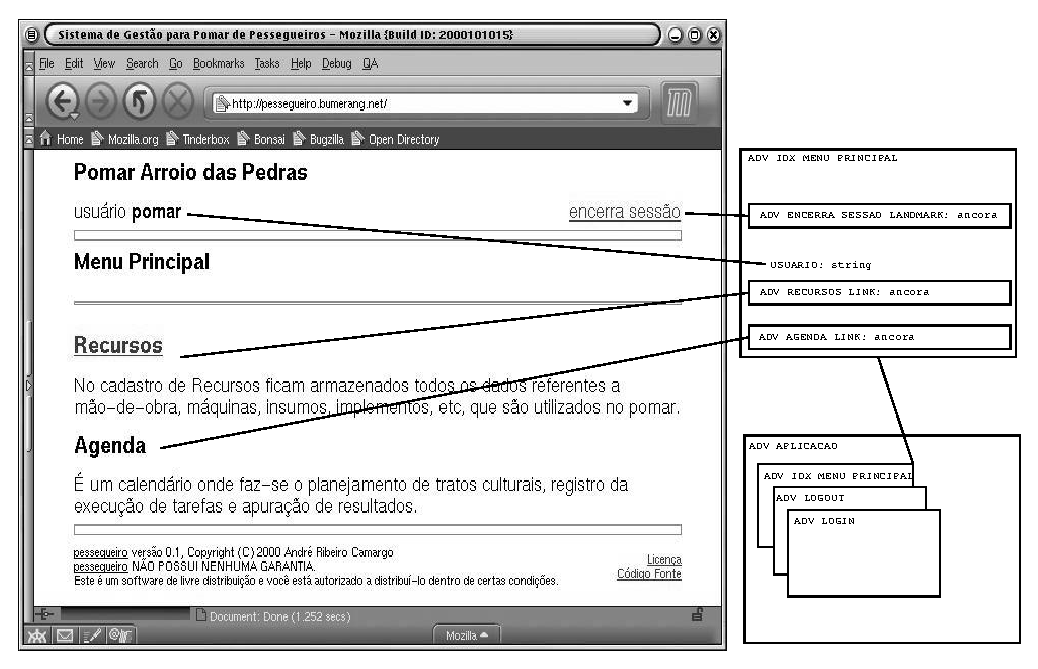
\includegraphics{diagramas/ilust_adv_idx_menu_principal.eps}} \par}
\caption{Interface para o usu�rio do ADV IDX MENU PRINCIPAL}
\label{fimenuprincipal}
\end{figure}

\paragraph{A interface para o usu�rio do ADV CTX CRIA HUMANO � apresentado na
Figura \ref{ficriahumano}.}

\begin{figure}[!h]
{\centering \resizebox*{\textwidth}{0.8\textheight}{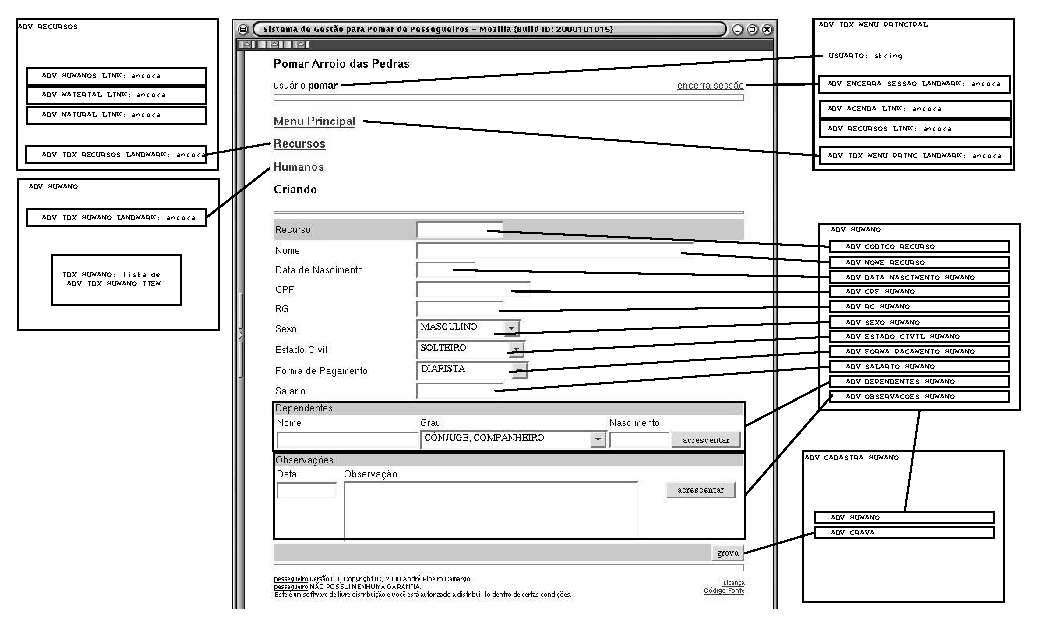
\includegraphics{diagramas/ilust_adv_ctx_cria_humano.eps}} \par}
\caption{Implementa��o do ADV CTX CRIA HUMANO}
\label{ficriahumano}
\end{figure}

\paragraph{Conv�m lembrar que os ADVs s�o objetos abstratos, sendo que a
especifica��o de sua interface (em HTML) � armazenada em arquivos
separados que s�o chamados de ``met�foras de interface''. O desenvolvedor
deve carregar a met�fora do ADV em quest�o, instanciar os ADVs aninhados e 
tornar percept�veis aqueles que o contexto da aplica��o requere. Feito isso,
o framework substitui as refer�ncias dos ADVs aninhados
por suas respectivas met�foras.}
\paragraph{A seguir apresento a especifica��o
em HTML da met�fora de interface do ADV HUMANO (este ADV � utilizado
sempre quando se deseja mostrar todos os dados sobre um Recurso Humano).
Note que h� ADVs aninhados (cujo nome est� entre um par de pontos de 
interroga��o). O resultado visual desta especifica��o � mostrado na figura 
\ref{fmetafora}.}

\verbatiminput{adv_humano.html}

\begin{figure}[!h]
{\centering \resizebox*{0.7\textwidth}{0.4\textheight}{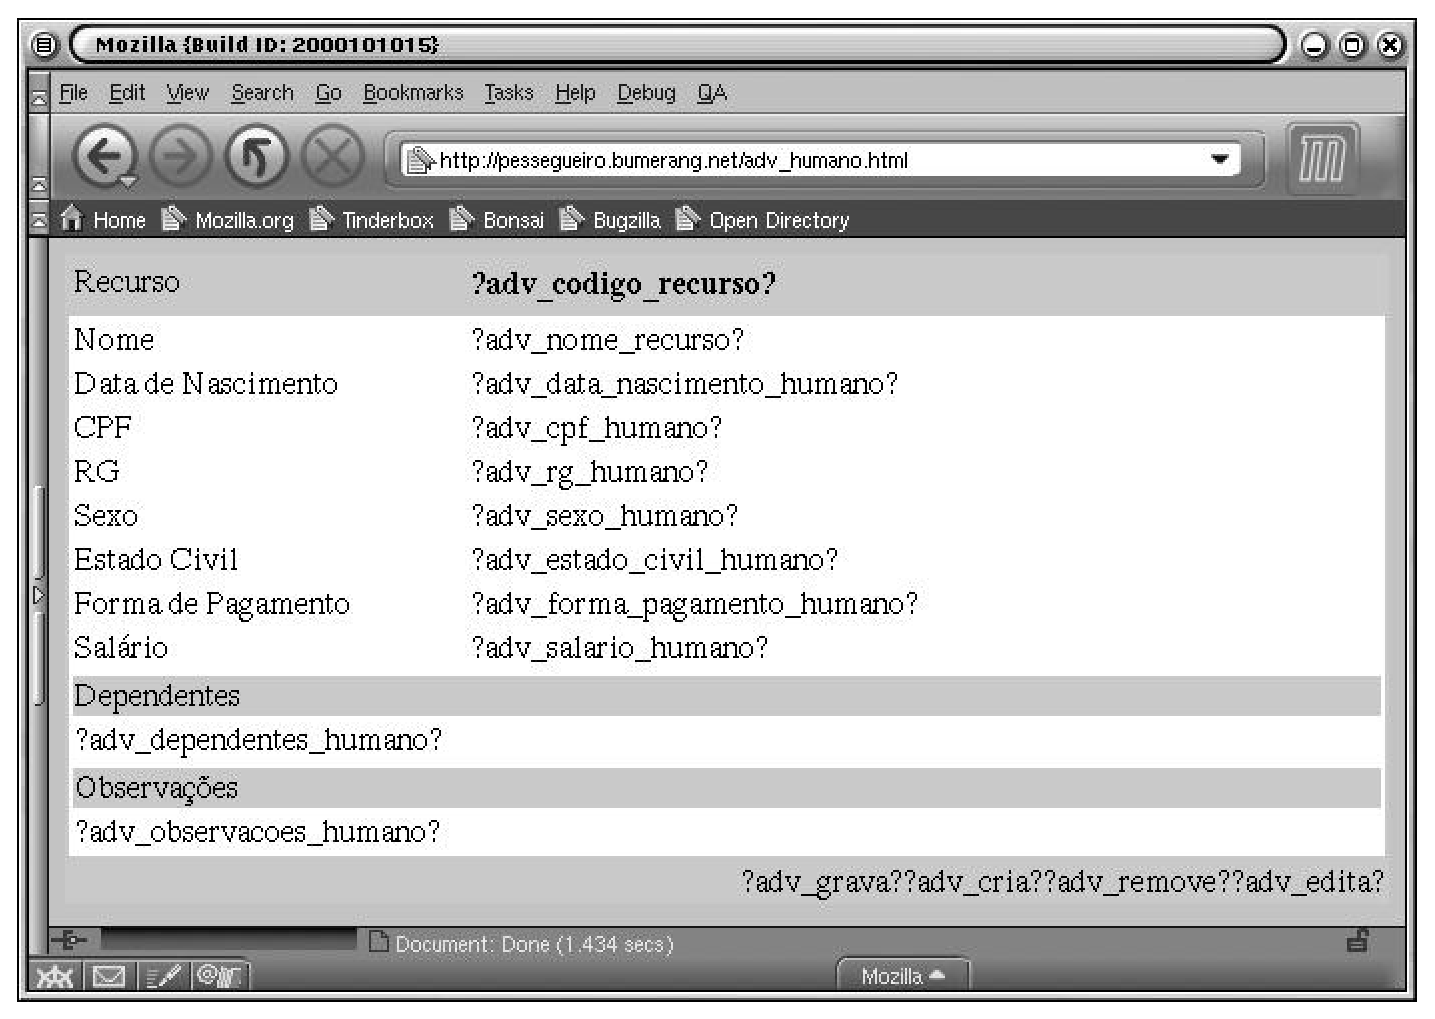
\includegraphics{diagramas/adv_humano.eps}} \par}
\caption{Met�fora de interface para o ADV HUMANO}
\label{fmetafora}
\end{figure}

\paragraph{Note que como a OOHDM pede, h� uma separa��o entre a parte l�gica
e a parte visual da aplica��o. A implementa��o deste modelo em PHP orientado
a objetos, foi muito prejudicado devido a m� implementa��o de polimorfismo
nesta ferramenta. Acredito que a implementa��o com Java Server Pages seja
mais tranq�ila, at� mesmo porque, JSP trabalha com esse conceito de separar
a apresenta��o da implementa��o.}

\section{A constru��o do caso de uso ``Planejar tratos culturais''}

\paragraph{O planejamento de tratos culturais se d� atrav�s da estimativa
de custo para realiza��o do mesmo. 
A Figura \ref{fcuptc} ilustra os casos de uso de sistema que o caso de uso 
de neg�cio ``Planejar tratos culturais'' possui.}

\begin{figure}[!h]
{\centering \resizebox*{0.7\textwidth}{0.5\textheight}{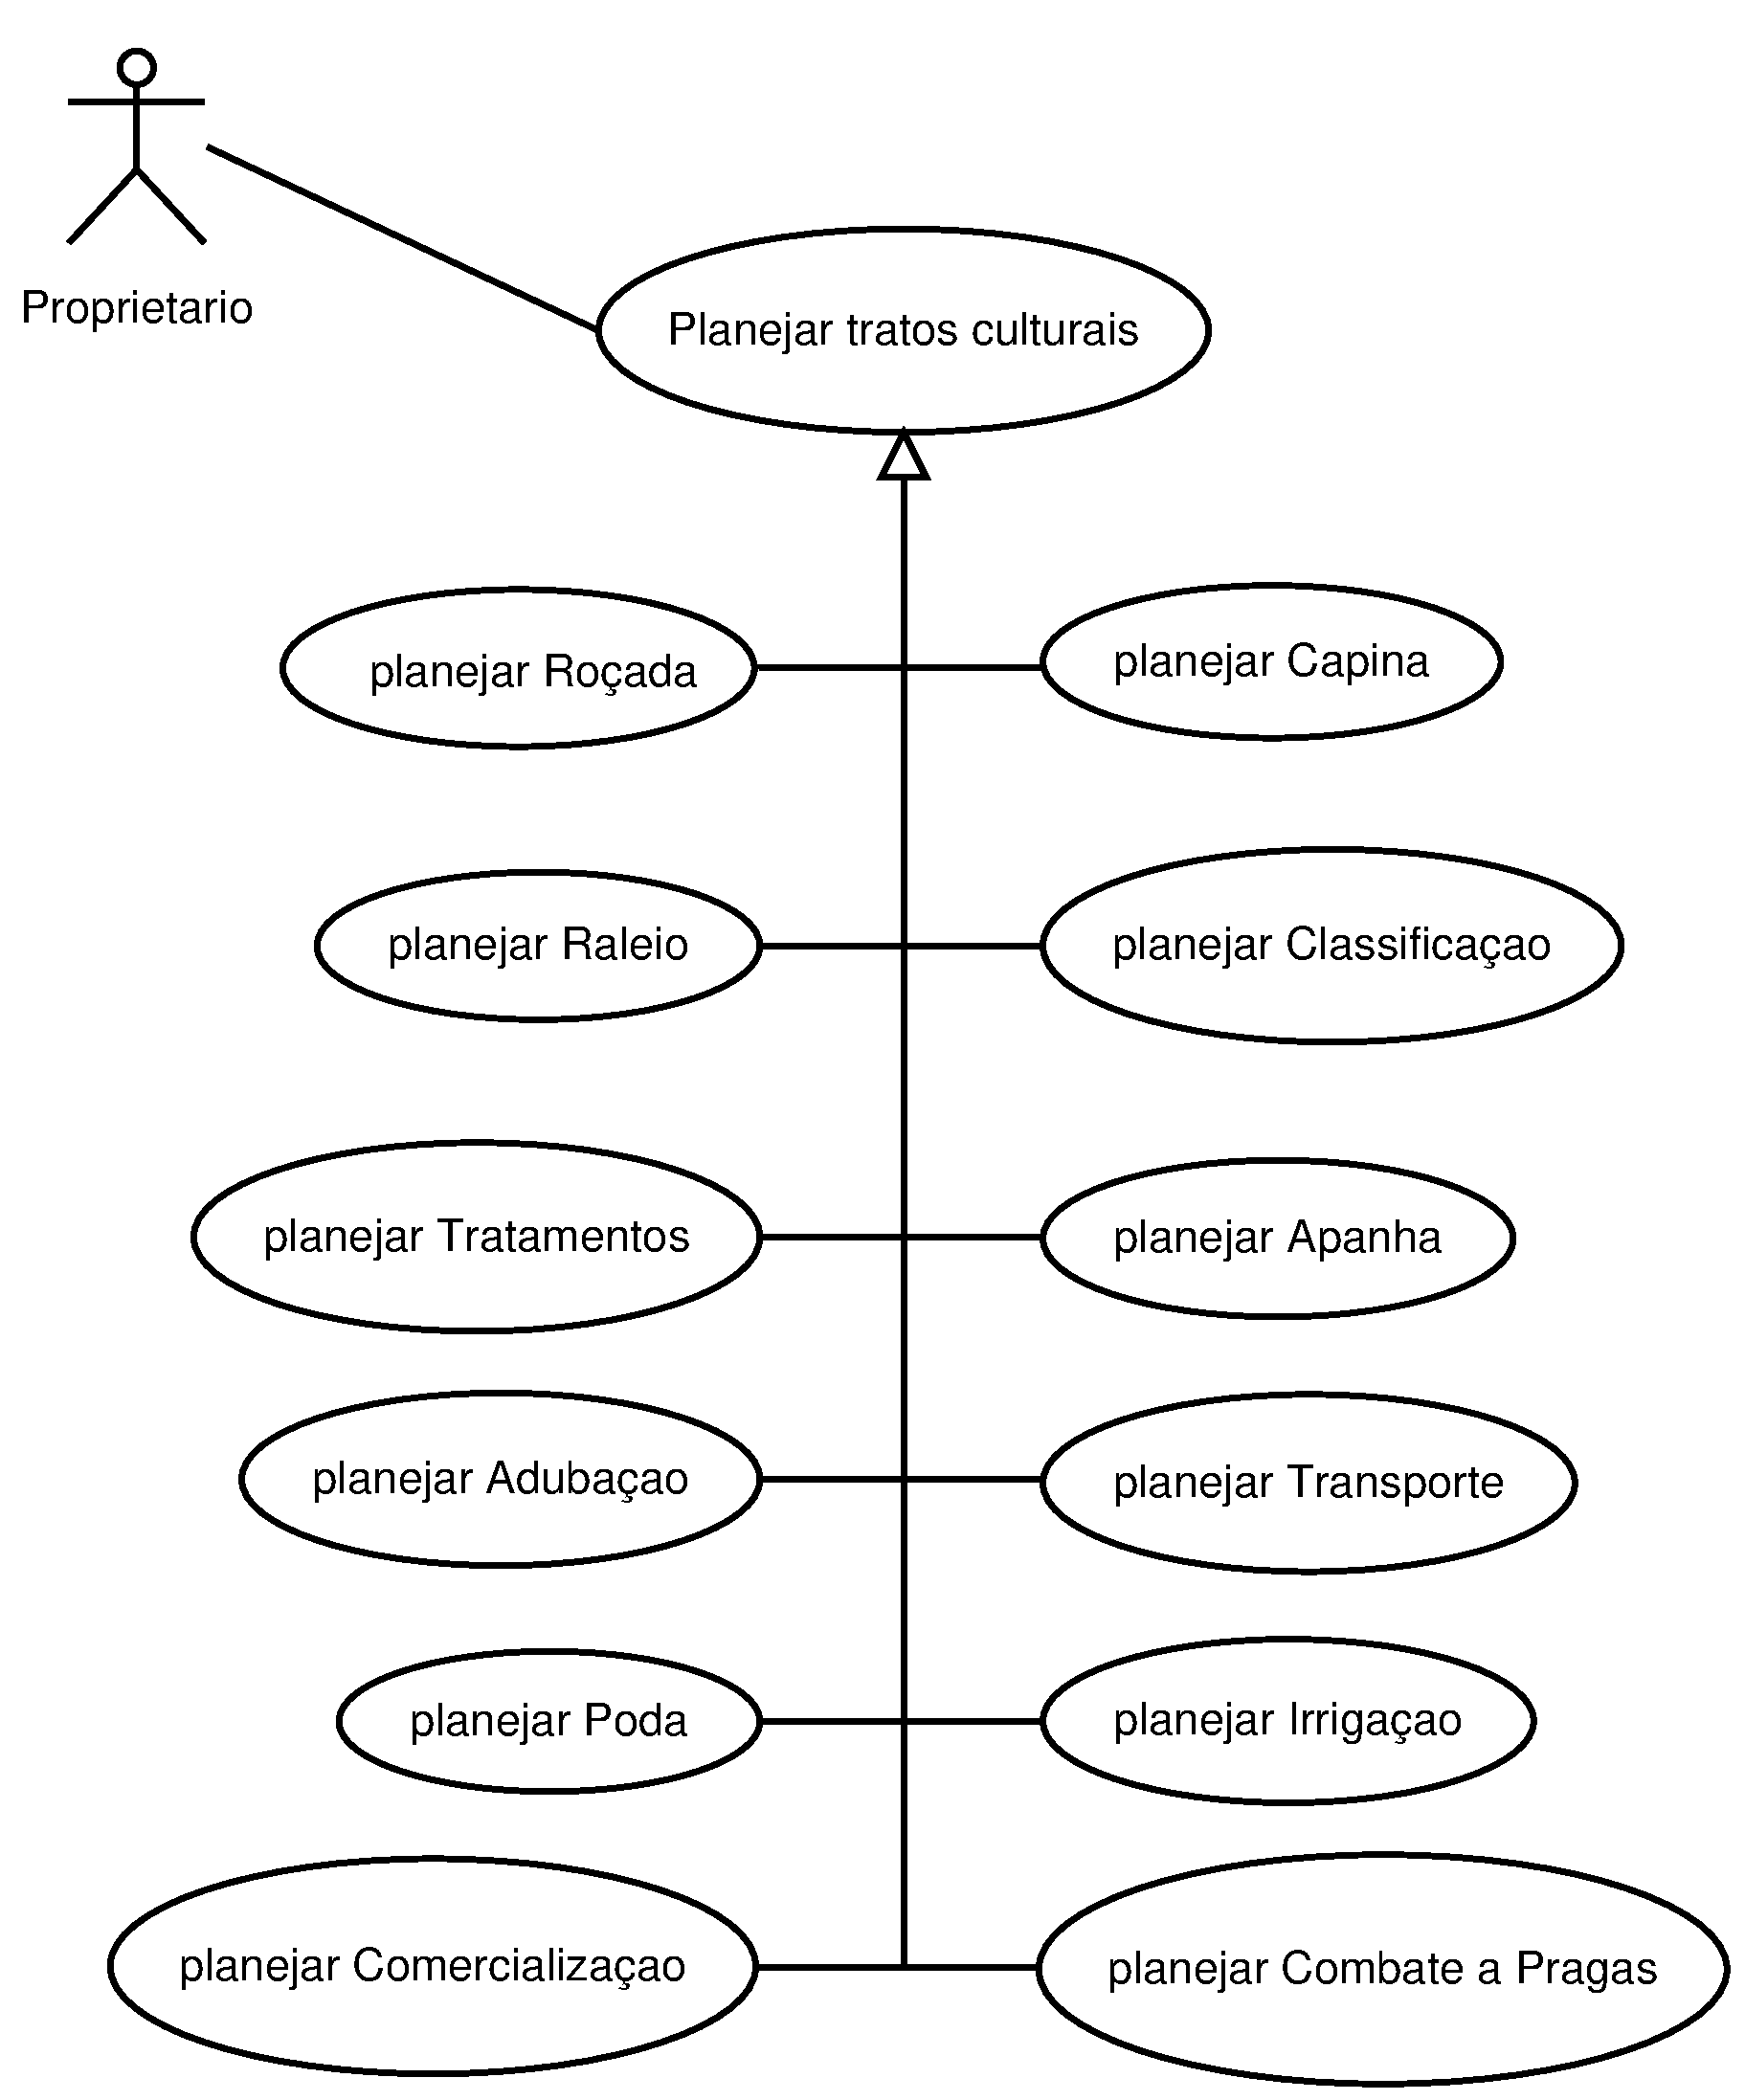
\includegraphics{diagramas/casodeusoplanejartratosculturais.eps}} \par}
\caption{Caso de uso de ``Planejar tratos culturais''}
\label{fcuptc}
\end{figure}

\paragraph{Considera��es:}
\begin{itemize}
\item Toda estimativa de trato cultural � feita por lote.
\item O custo estimado do recurso m�quina � feito multiplicando-se a quantidade de horas de
servi�o necess�rias para execu��o da tarefa pelo valor da hora de servi�o 
estipulada pelo propriet�rio do pomar.
\item O custo estimado de recursos humanos (m�o-de-obra) � feito multiplicando-se a quantidade
de horas de servi�o necess�rias para execu��o da tarefa pelo valor da hora de
m�o-de-obra.
\item O custo estimado de recurso insumo � feito multiplicando-se a dosagem do insumo por hectare
pelo custo unit�rio de aquisi��o do mesmo (em kg ou l).
\item Optou-se por n�o estimar Recursos materiais da classe utens�lios.
\end{itemize}

\paragraph{Os casos de uso de sistema est�o textualizados abaixo:}

\begin{itemize}

\item \textbf{Planejar Ro�ada}\\
A estimativa de custo de Ro�ada Manual � feito calculando-se o
custo com recursos humanos.\\
A estimativa de custo de Ro�ada Mec�nica � feito somando o custo com
recurso m�quina e humano.

\item \textbf{Planejar Raleio}\\
Estima-se Raleio calculando a utiliza��o de recursos
humanos necess�rios para execu��o do trato cultural.

\item \textbf{Planejar Tratamentos}\\
A estimativa do custo de Tratamento � feito multiplicando-se o n�mero
de aplica��es planejadas pelo custo por hectare de uma aplica��o. O custo de 
uma aplica��o � a soma do custo de distribui��o e o custo com insumos. O 
custo de distribui��o � a soma do custo da distribui��o manual com o custo da 
distribui��o mecanizada.
A distribui��o manual � feita com recursos humanos, enquanto que, distribui��o
tratorizada utiliza recurso trator. O custo com insumos � feito multiplicando-se
a �rea do lote pelo somat�rio do custo de cada insumo (calda) por hectare. O custo de 
cada insumo � o custo de cada recurso insumo utilizado por hectare. Na 
pulveriza��o, o somat�rio do custo de cada insumo poderia ser chamado de custo 
da calda.

\item \textbf{Planejar Aduba��o}\\
Planejado da mesma forma de um Tratamento.

\item \textbf{Planejar Poda}\\
A poda � um trato cultural executado de forma manual, � estimado conforme
a utiliza��o de recursos humanos para efetu�-la.

\item \textbf{Planejar Capina}\\
Capina manual planeja-se conforme a necessidade de recursos humanos para efetu�-la, 
enquanto que, na capina mec�nica estima-se a utiliza��o de recursos
humanos e maquin�rios, j� o planejamento da capina qu�mica segue os moldes da
estimativa de um tratamento.

\item \textbf{Planejar Combate a Pragas}\\
O planejamento do combate a pragas � semelhante a estimativa de um tratamento.

\item \textbf{Planejar Irriga��o}\\
A estimativa do custo de Irriga��o � o somat�rio dos custos estimados de �gua,
bombeamento, recursos humanos e reposi��o de pe�as/manuten��o de equipamentos.
Para estimarmos o custo d'�gua e bombeamento � preciso definir previamente a
necessidade d'�gua do lote. Esta necessidade d'�gua do lote � o produto da necessidade
di�ria de �gua por planta (em \( m^{3} \)) pelo n�mero de plantas do lote.
Assim, o custo estimado com �gua � a necessidade d'�gua do lote multiplicado
pelo valor do \( m^{3} \) d'�gua (obs.: caso a �gua seja comprada, se n�o for,
n�o h� custo com �gua). O custo estimado de bombeamento � feito multiplicando-se
o tempo de bombeamento pelo valor da hora de bombeamento. O tempo de bombeamento
(em horas) � o quociente da necessidade d'�gua do lote (em \( m^{3} \)) pela
capacidade de recalque d'�gua da bomba (\( m^{3} \)/h). A estimativa do custo
com reposi��o de pe�as/manuten��o de equipamentos � uma porcentagem calculada
sobre o somat�rio dos custo de bombeamento e recursos humanos, a porcentagem 
padr�o para c�lculo � de 5\%, podendo ser modificada.

\item \textbf{Planejar Apanha}\\
O custo estimado de apanha � o produto da produtividade m�dia 
estimada por hectare, multiplicada pelo valor de apanha/kg.

\item \textbf{Planejar Transporte Interno}\\
O custo estimado de transporte interno � a soma da expectativa de
uso de recursos materiais  com a expectativa de uso de recursos humanos por 
hectare multiplicado pela �rea a ser colhida.

\item \textbf{Planejar Classifica��o}\\
O custo estimado de classifica��o � obtido pelo produto
da produ��o bruta estimada (em kg) pelo custo de classifica��o por
kg.

\item \textbf{Planejar Comercializa��o}\\
A estimativa de comercializa��o � o produto da expectativa
de produ��o a ser vendida �s ind�strias e/ou com�rcio \emph{in natura} pelo 
pre�o de mercado da fruta com base na safra anterior e �s poss�veis varia��es
que possam vir a ocorrer em fun��o de altera��es de oferta e procura ou mesmo 
na varia��o monet�ria.

\end{itemize}

\subsection{Modelagem conceitual}

\paragraph{A modelagem conceitual do caso de uso ``Planejar Tratos Culturais''
produziu o diagrama de classes conceituais da Figura \ref{fmcptc}.}

\begin{figure}[!h]
{\centering \resizebox*{\textwidth}{0.9\textheight}{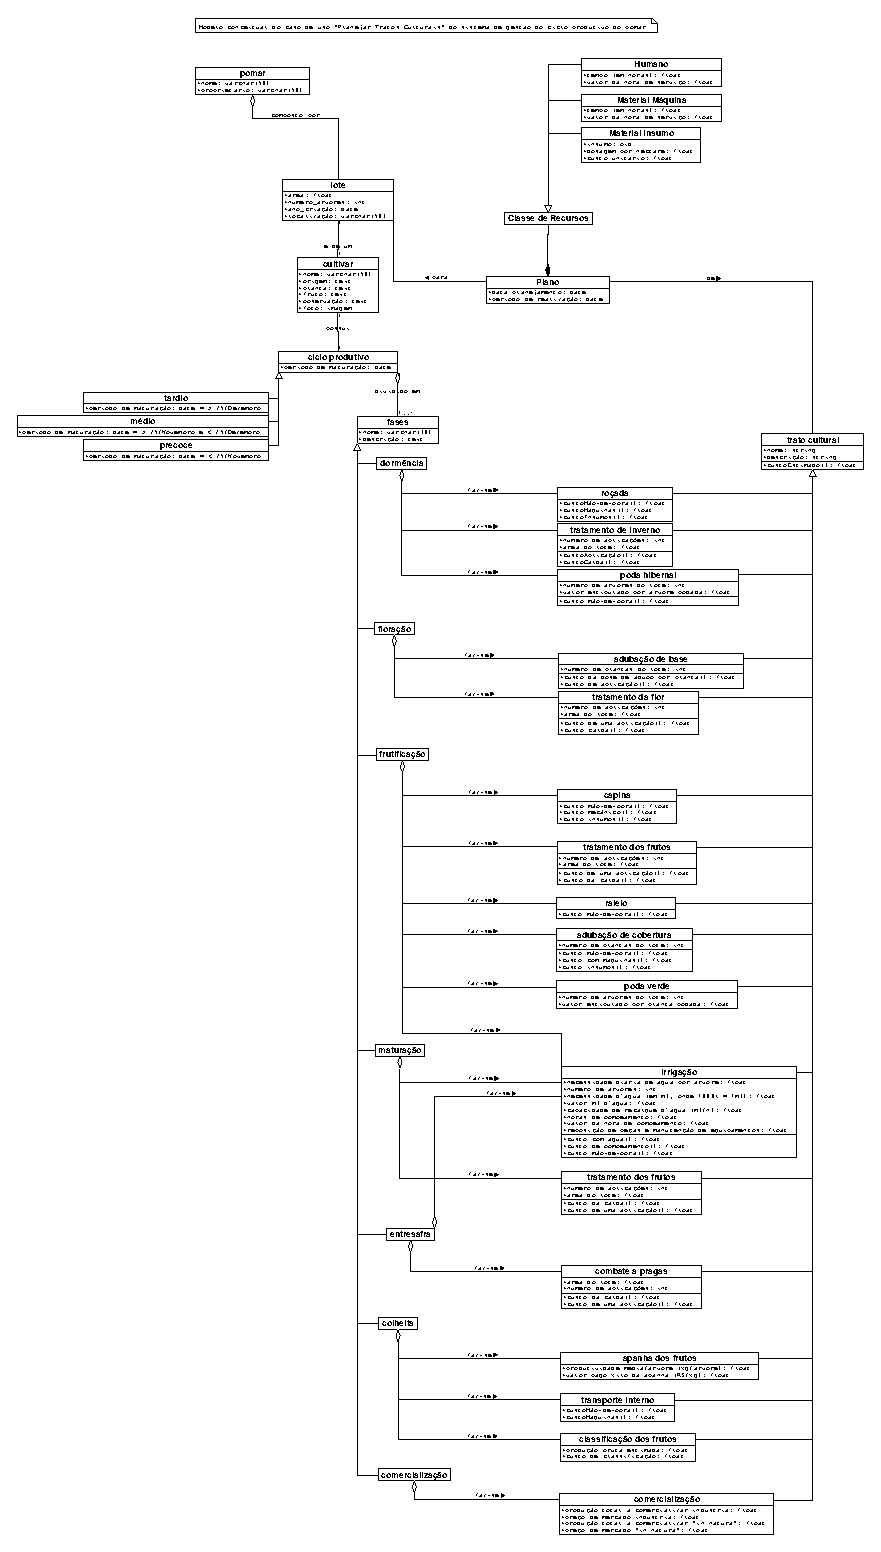
\includegraphics{diagramas/plan_rec_modelo_conceitual.eps}} \par}
\caption{Modelo conceitual do caso de uso ``Planejar Tratos Culturais''}
\label{fmcptc}
\end{figure}

\subsection{Projeto navegacional}

\paragraph{Por ser um caso de uso simples, a navega��o � pouca, como pode se 
demonstrado no seu esquema navegacional (Figura \ref{fenptc}) e diagrama de contextos
(Figura \ref{fdcptc}).}

\begin{figure}[!h]
{\centering \resizebox*{\textwidth}{0.9\textheight}{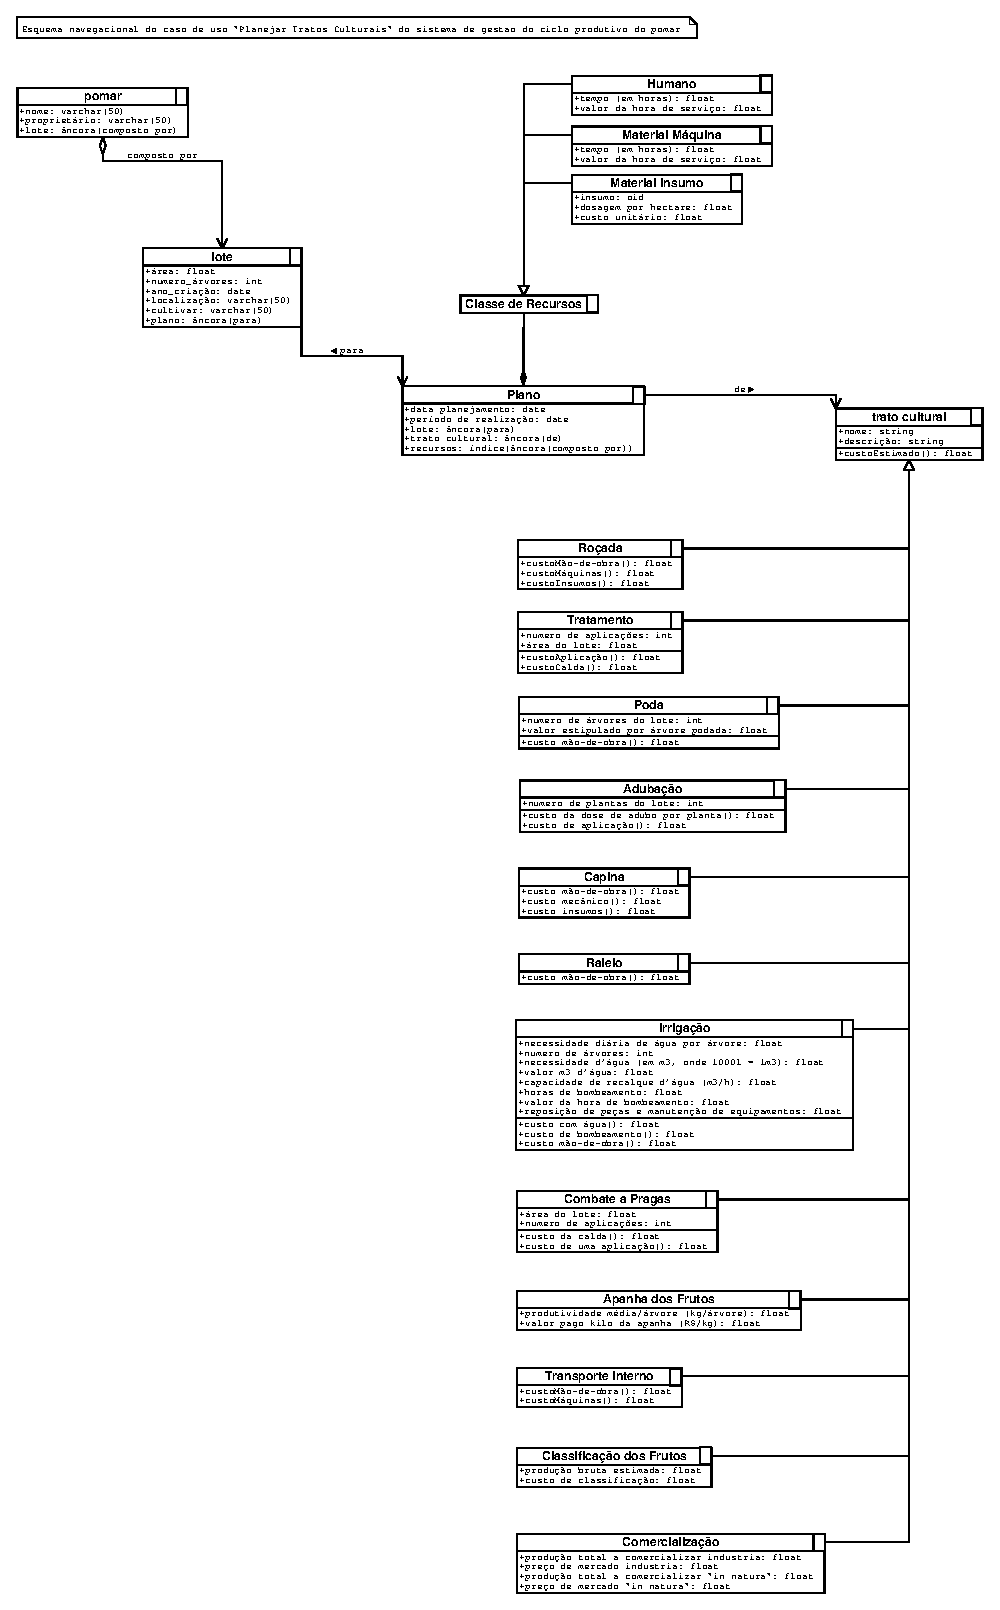
\includegraphics{diagramas/plan_rec_esquema_navegacional.eps}} \par}
\caption{Esquema navegacional do caso de uso ``Planejar Tratos Culturais''}
\label{fenptc}
\end{figure}

\begin{figure}[!h]
{\centering \resizebox*{\textwidth}{0.9\textheight}{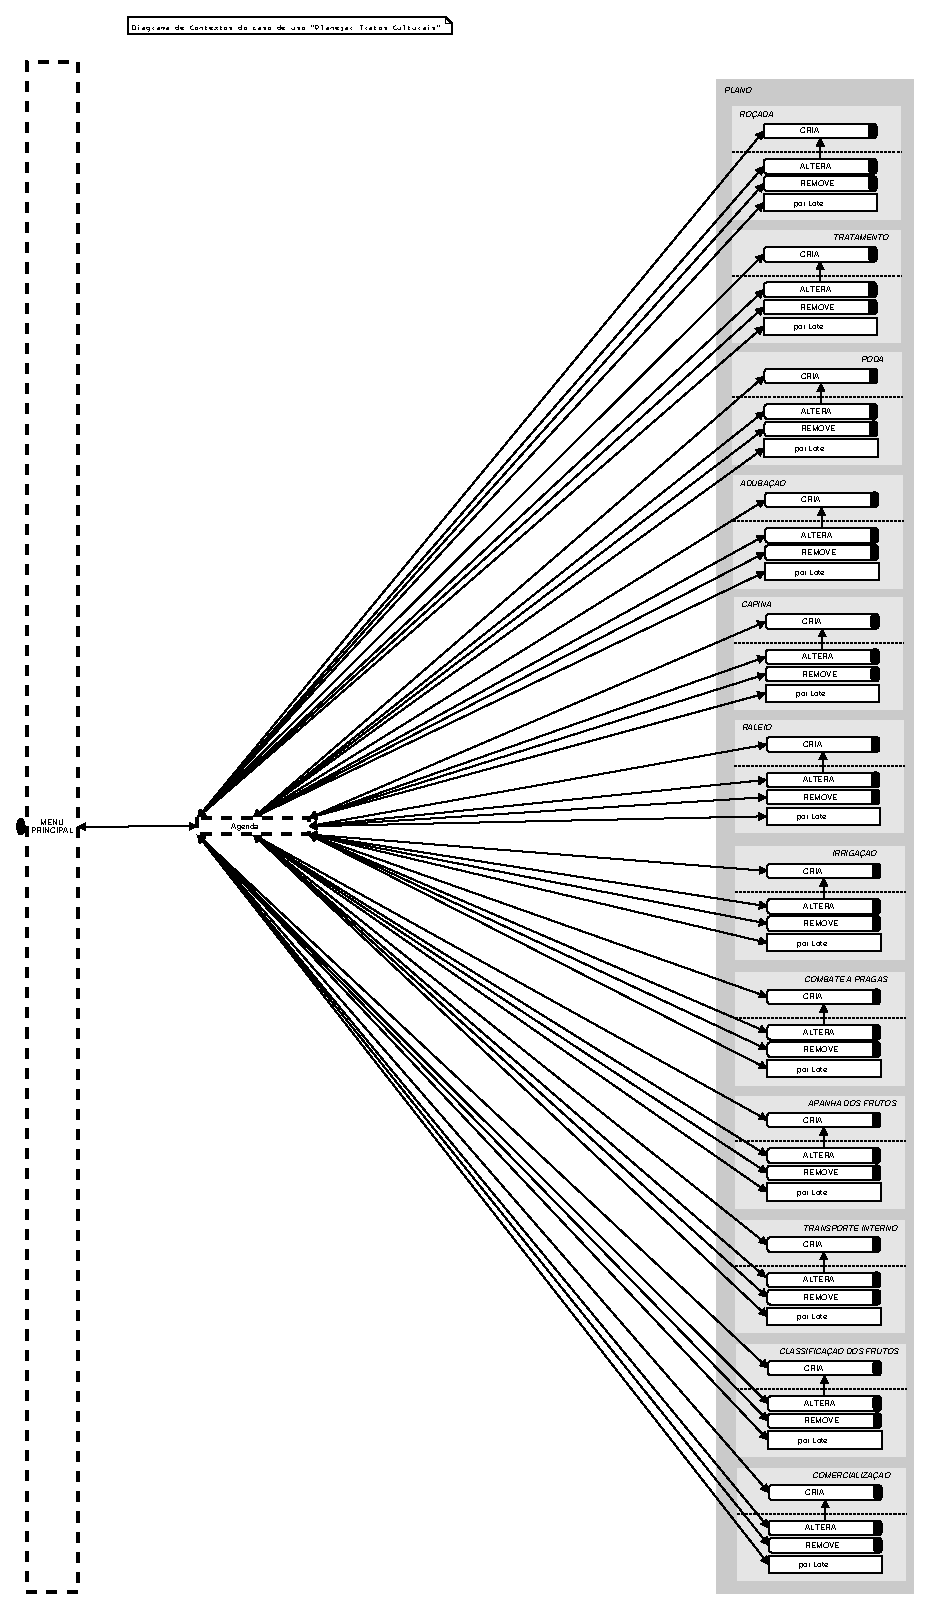
\includegraphics{diagramas/plan_rec_diag_contextos.eps}} \par}
\caption{Diagrama de contextos do caso de uso ``Planejar Tratos Culturais''}
\label{fdcptc}
\end{figure}

\subsection{Projeto de interface abstrata}
\paragraph{Os ADVs do caso de uso ``Planejar Tratos Culturais'' encontram-se
documentados na Figura \ref{fadvptc}.}

\begin{figure}[!h]
{\centering \resizebox*{\textwidth}{0.9\textheight}{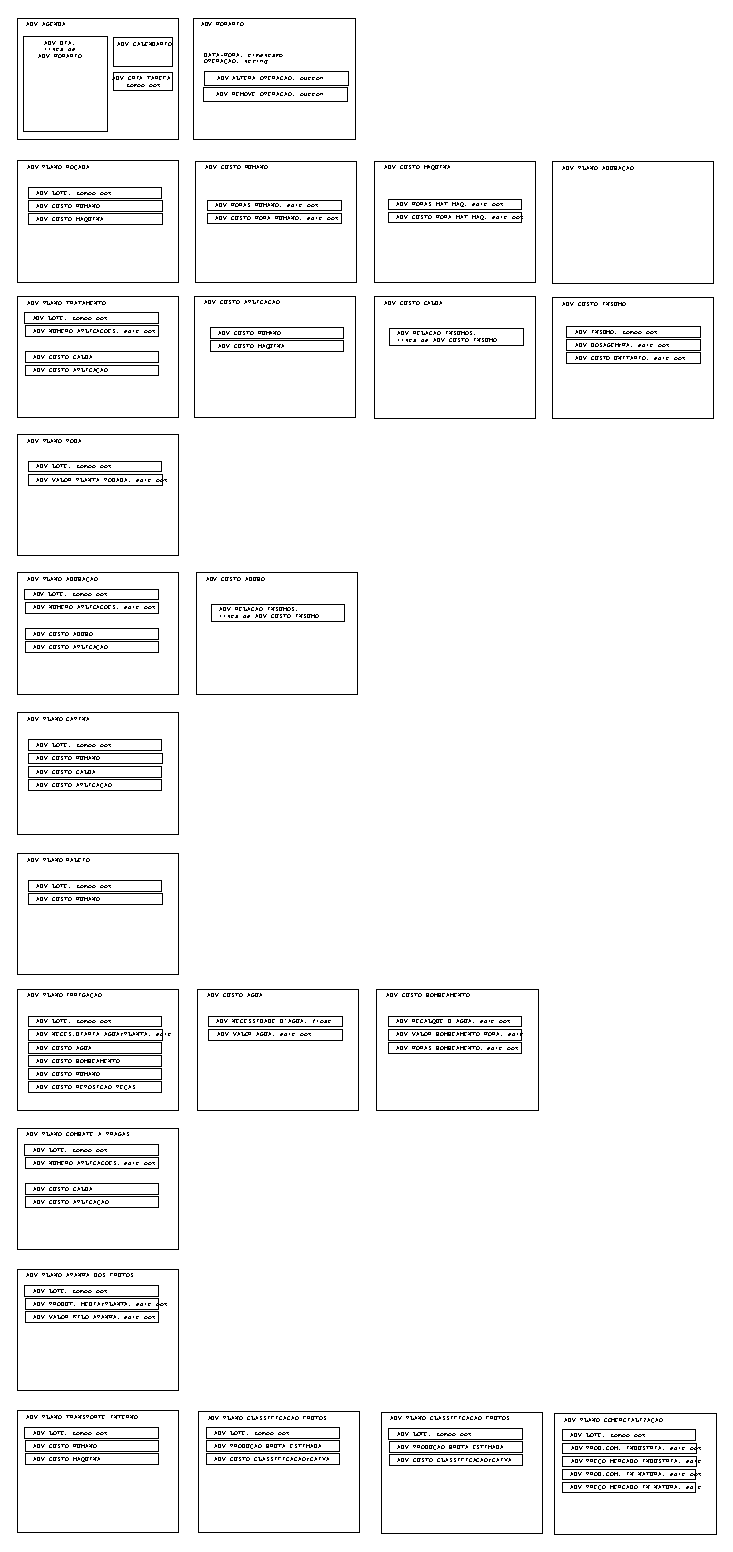
\includegraphics{diagramas/plan_rec_adv.eps}} \par}
\caption{Abstract Data Views do caso de uso ``Planejar Tratos Culturais''}
\label{fadvptc}
\end{figure}

\section{A constru��o do caso de uso ``Registrar tarefas''}
\paragraph{A execu��o de tratos culturais se d� atrav�s de tarefas que 
utilizam recursos do pomar. Conforme pode ser visto na Se��o 
\ref{sec:decomposicao}, decompus
os tratos culturais em tarefas para facilitar a constru��o da aplica��o e o 
registro das mesmas por parte dos usu�rios.
A Figura \ref{fcurt} ilustra os casos de uso de sistema que o caso de uso
de neg�cio ``Registrar tarefas''.}

\begin{figure}[!h]
{\centering \resizebox*{\textwidth}{0.6\textheight}{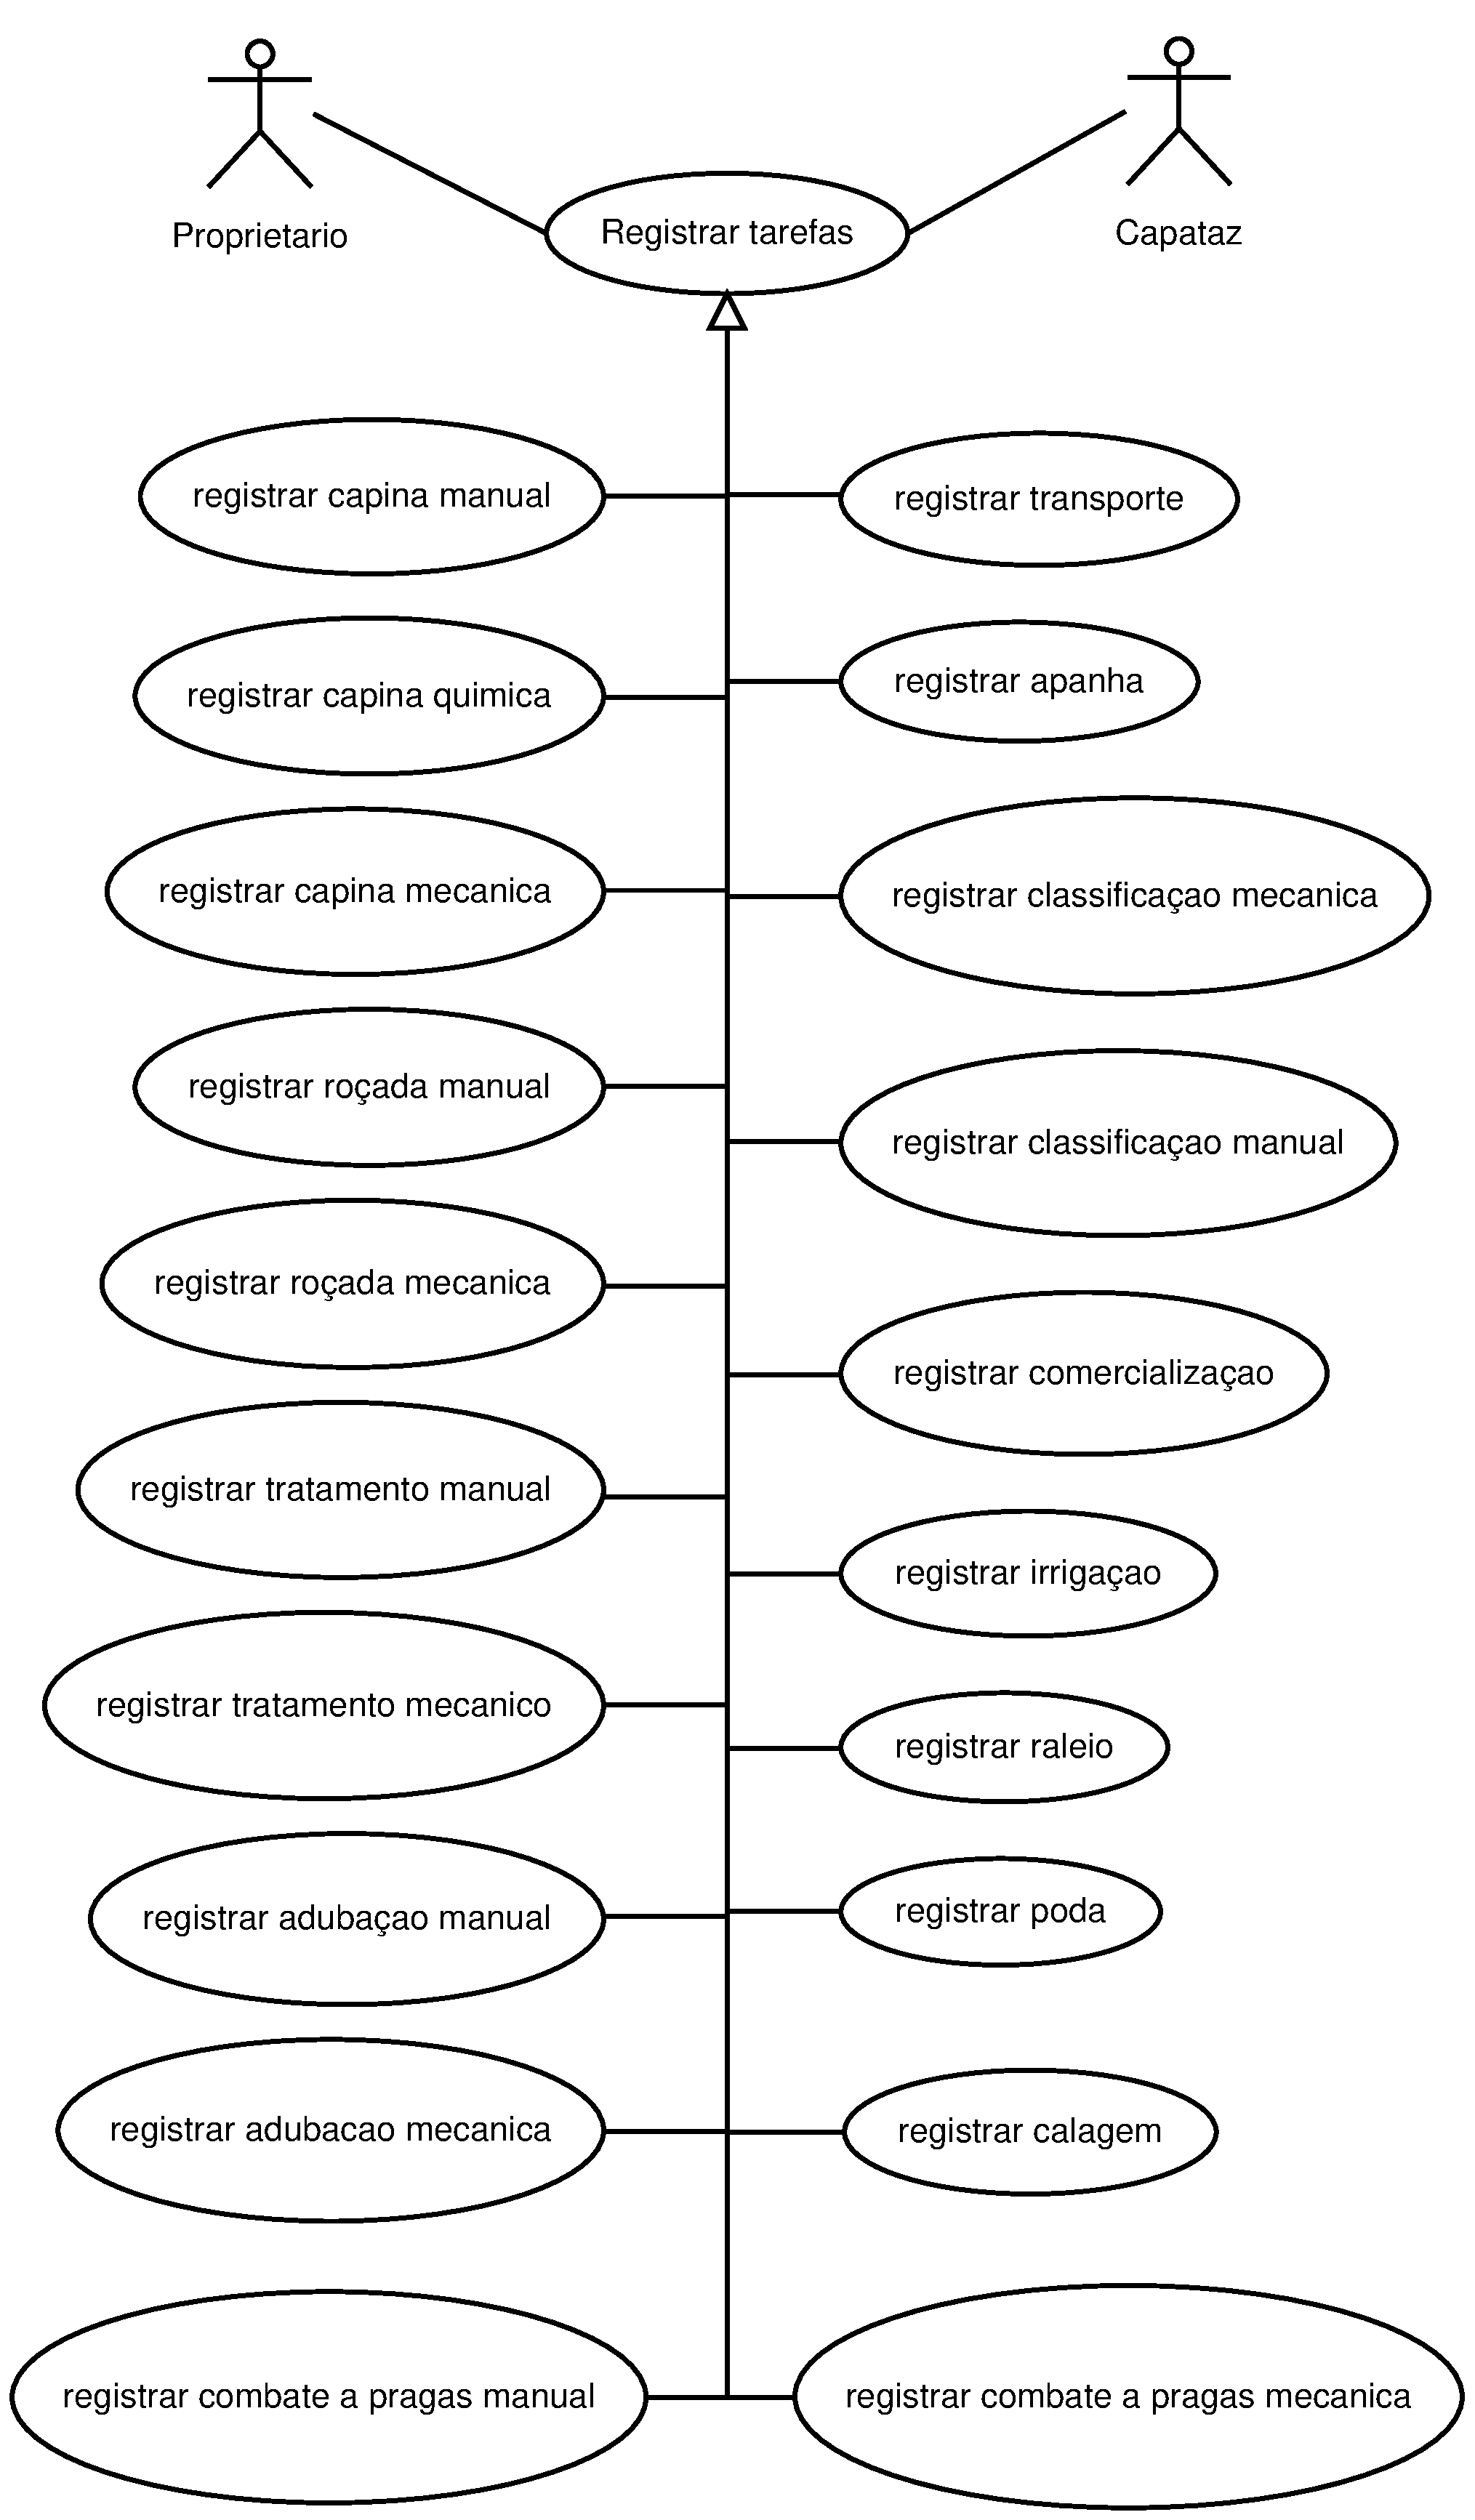
\includegraphics{diagramas/casodeusoregistrartarefas.eps}} \par}
\caption{Caso de uso de ``Registrar tarefas''}
\label{fcurt}
\end{figure}

\paragraph{Considera��es:}
\begin{itemize}
\item O registro do uso de recursos humanos � feito documentando-se o 
tempo ocupado (em horas), o valor da hora trabalhada (hora normal 
e hora extra) com ou sem insalubridade e/ou periculosidade.
\item O registro do uso de um recurso material m�quina � feito anotando-se 
o tempo, em horas, e o valor da hora trabalhada.
\item O registro do recurso insumo � feito especificando-se o nome do 
insumo, e a quantidade utilizada.
\item O registro de uso do recurso material utens�lio e implemento n�o � feito.
\end{itemize}

\paragraph{Os casos de uso de sistema est�o textualizados abaixo:}

\begin{itemize}
\item \textbf{Registrar Capina Manual}\\
Registra-se o uso de recursos humanos;
\item \textbf{Registrar Capina Mec�nica}\\
Registra-se a utiliza��o de recursos humanos e m�quinas;
\item \textbf{Registrar Capina Qu�mica}\\
Registra-se o uso de recursos humanos, m�quinas e insumos;
\item \textbf{Registrar Ro�ada Manual}\\
Registra-se a utiliza��o de recursos humanos;
\item \textbf{Registrar Ro�ada Mec�nica}\\
Registra-se o uso de recursos humanos e m�quinas;
\item \textbf{Registrar Tratamento Manual}\\
Registra-se a utiliza��o de recursos humanos;
\item \textbf{Registrar Tratamento Mec�nico}\\
Registra-se o uso de recursos humanos, m�quinas e insumos;
\item \textbf{Registrar Aduba��o Manual}\\
Registra-se a utiliza��o de recursos humanos e insumos;
\item \textbf{Registrar Aduba��o Mec�nica}\\
Registra-se o uso de recursos humanos, m�quinas e insumos;
\item \textbf{Registrar Combate a Pragas Manual}\\
Registra-se a utiliza��o de recursos humanos e insumos;
\item \textbf{Registrar Combate a Pragas Mec�nica}\\
Registra-se o uso de recursos humanos, m�quinas e insumos;
\item \textbf{Registrar Poda}\\
Registra-se a utiliza��o de recursos humanos;
\item \textbf{Registrar Raleio}\\
Registra-se o uso de recursos humanos;
\item \textbf{Registrar Irriga��o}\\
Registra-se a utiliza��o de recursos humanos e m�quinas;
\item \textbf{Registrar Apanha}\\
O registro da apanha de fruto � feito anotando-se o tempo (em horas)
e a quantidade (em kg) que cada pe�o conseguiu apanhar.
\item \textbf{Registrar Transporte}\\
O registro do transporte interno da colheita � feito anotando-se
a quantidade transportada por lote e o tempo (em horas) utilizado
dos recursos trator e humano.
\item \textbf{Registrar Classifica��o Manual}\\
O registro da tarefa de classifica��o manual � feito anotando-se o tempo
(em horas) trabalhado por cada recurso humano e a quantidade (em kg)
classificada nesse tempo.
\item \textbf{Registrar Classifica��o Mec�nica}\\
Registra-se a utiliza��o de recursos humanos, o tempo de trabalho da m�quina
e a quantidade (em kg) classificada.
\item \textbf{Registrar Comercializa��o}\\
O registro da comercializa��o da produ��o � feito anotando-se a
quantidade (em kg) entregue, o valor unit�rio,
o comprador, o respons�vel pela entrega, os dados do transportador (nome, placa do caminh�o)
e os vencimentos (data e valor).
\end{itemize}

\subsection{Modelagem conceitual}

\paragraph{O modelo conceitual do caso de uso de neg�cio ``Registrar Tarefas''
est� representado na Figura \ref{fmcrt}.}

\begin{figure}[!h]
{\centering \resizebox*{\textwidth}{0.9\textheight}{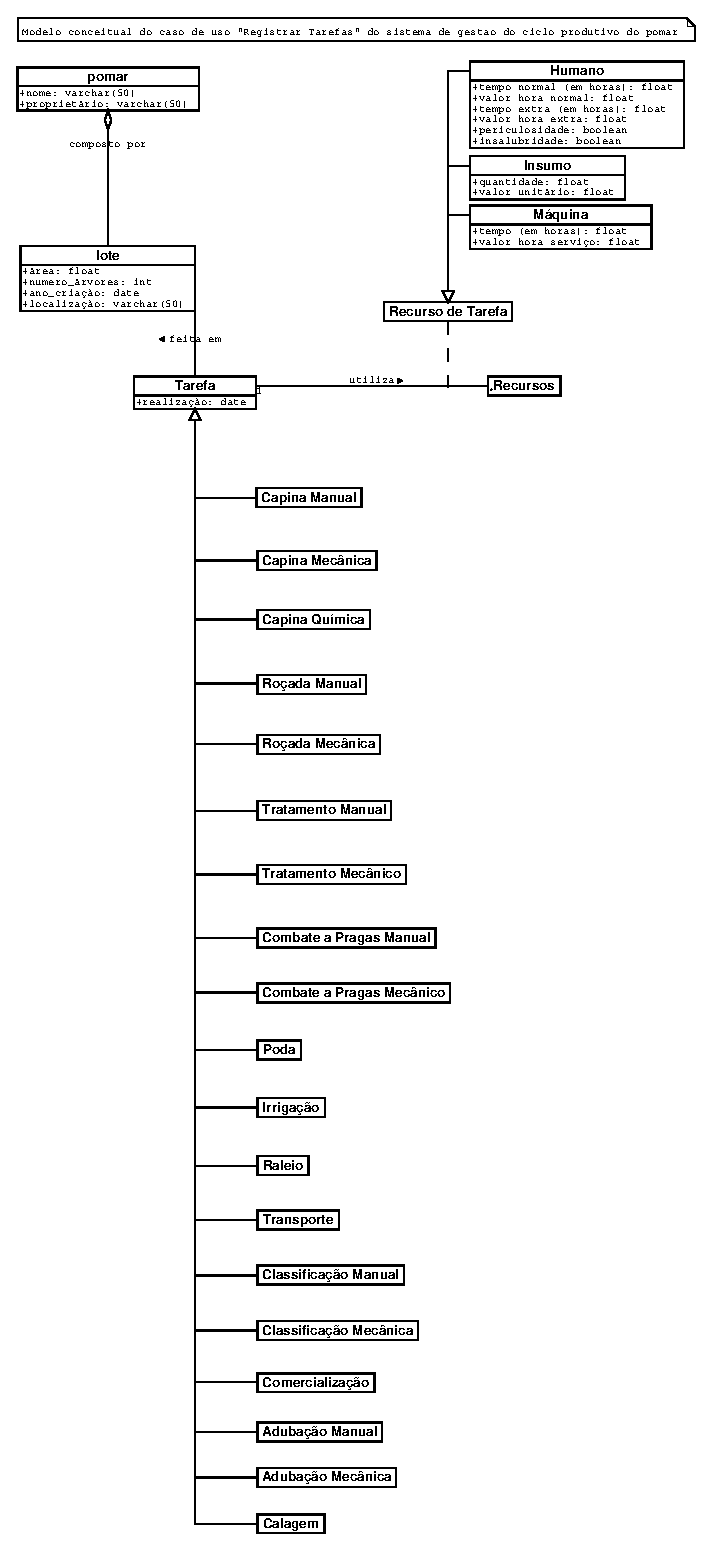
\includegraphics{diagramas/reg_tar_modelo_conceitual.eps}} \par}
\caption{Modelo conceitual do caso de uso de ``Registrar Tarefas''}
\label{fmcrt}
\end{figure}

\subsection{Projeto navegacional}

\paragraph{Baseado no modelo conceitual proposto anteriormente, foi criado 
o esquema navegacional da Figura \ref{fenrt} e o diagrama de contextos da 
Figura \ref{fdcrt}.}

\begin{figure}[!h]
{\centering \resizebox*{\textwidth}{0.5\textheight}{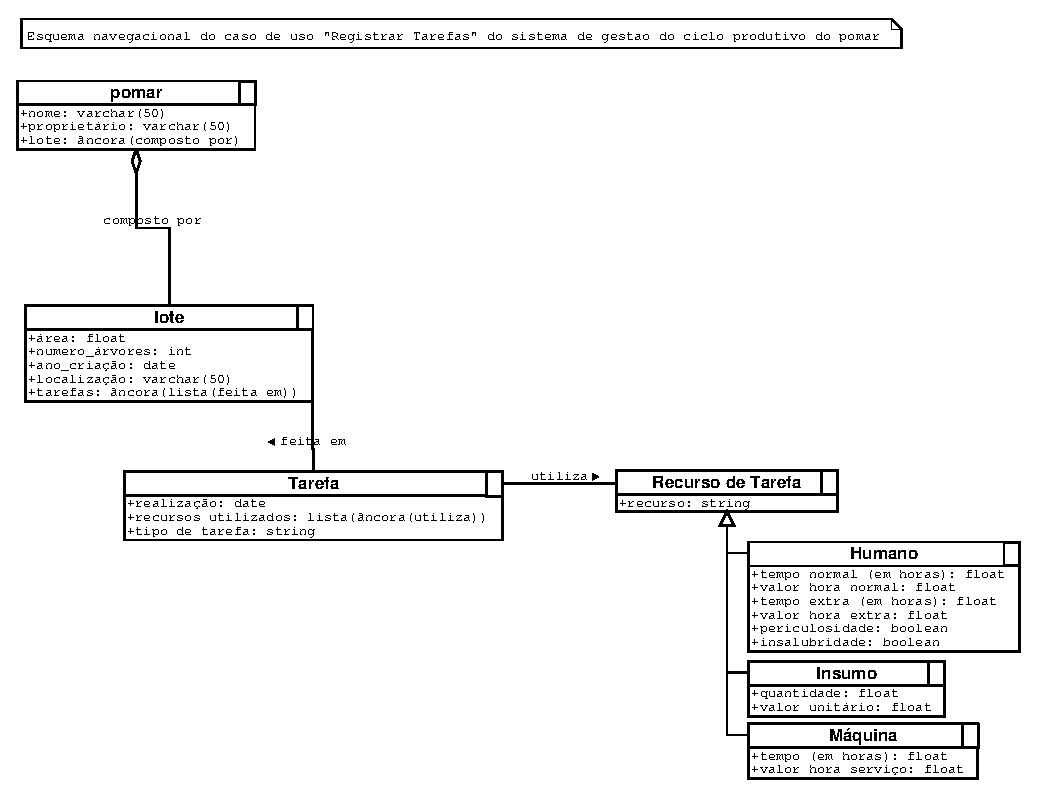
\includegraphics{diagramas/reg_tar_esquema_navegacional.eps}} \par}
\caption{Esquema navegacional do caso de uso de ``Registrar Tarefas''}
\label{fenrt}
\end{figure}

\begin{figure}[!h]
{\centering \resizebox*{\textwidth}{0.3\textheight}{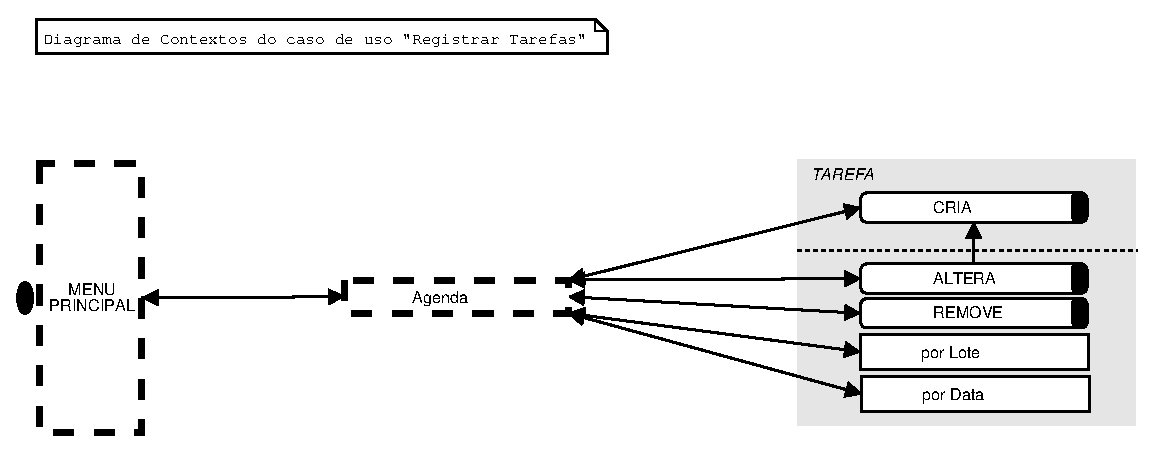
\includegraphics{diagramas/reg_tar_diag_contextos.eps}} \par}
\caption{Diagrama de contextos do caso de uso de ``Registrar Tarefas''}
\label{fdcrt}
\end{figure}

\subsection{Projeto de interface abstrata}

\paragraph{A Figura \ref{fadvrt} ilustra os Abstract Data Views deste caso de 
uso.}

\begin{figure}[!h]
{\centering \resizebox*{\textwidth}{0.3\textheight}{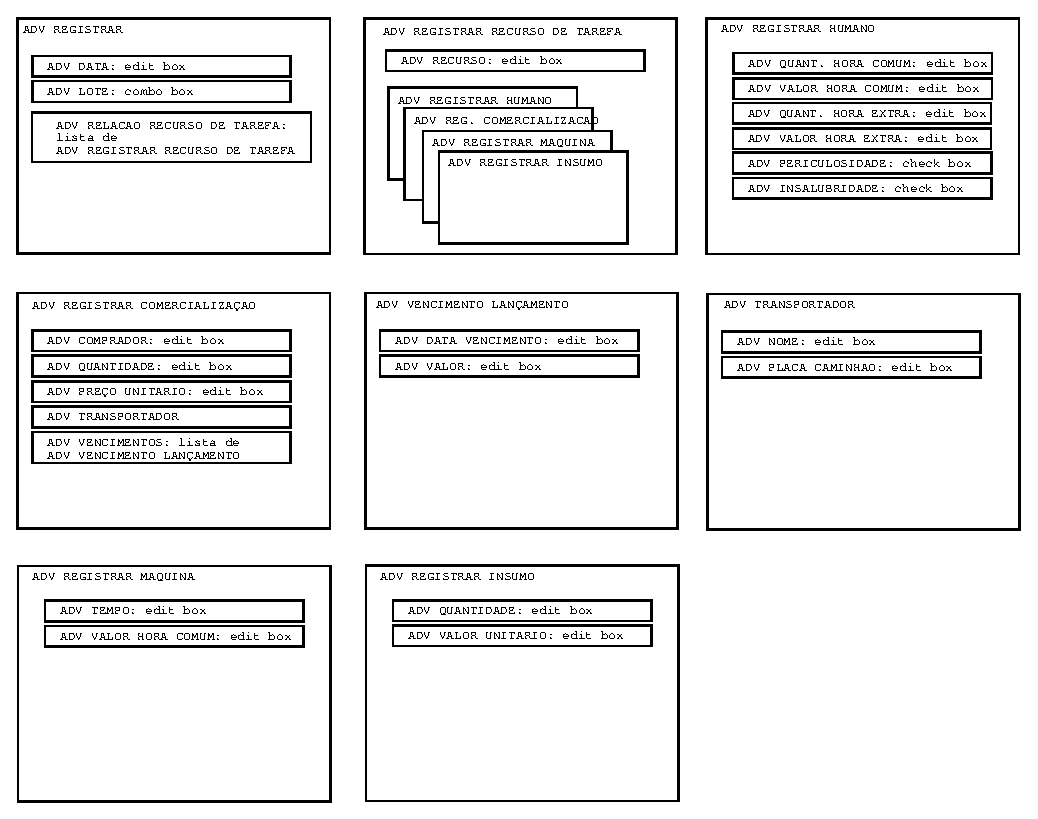
\includegraphics{diagramas/reg_tar_adv.eps}} \par}
\caption{ADVs do caso de uso de ``Registrar Tarefas''}
\label{fadvrt}
\end{figure}

\section{A constru��o do caso de uso ``Apurar Resultados''}

\paragraph{Apurar resultados � o �ltimo caso de neg�cio deste sistema de
gest�o para pomar de pessegueiros.}
\paragraph{Em conversa com o Sr. Adelci, ficou decidido que a necessidade
prim�ria � obter relat�rios que mostrem:}
\begin{itemize}
\item Quanto foi gasto por recurso?\\O sistema deve ser capaz de gerar
extratos de quanto foi gasto por recursos dentro de um per�odo de tempo
especificado pelo usu�rio.
\item Qual foi o total colhido?\\O sistema deve ser capaz de gerar
relat�rio descriminados do total colhido por ciclo, cultivar e lote.
\item Relat�rio de vendas da safra\\O sistema deve ser capaz de gerar
relat�rio de vendas dentro de um per�odo especificado pelo usu�rio. Neste
relat�rio deveria conter dados como: para quem foi vendido, data da entrega,
por quanto foi entregue e qual � a previs�o de recebimentos.
\item Qual foi o resultado final?\\O sistema deve ser capaz de gerar
o relat�rio de resultado final por ciclo, lote e cultivar. Este relat�rio
consiste de um balan�o relacionando o valor da produ��o com o valor gasto
para produzir.
\item De quanto foi as perdas entre apanha e comercializa��o?\\
O sistema deve ser capaz de apontar quanto do p�ssego apanhado
� rejeitado at� a colheita.
\end{itemize}
\paragraph{A Figura \ref{fcuar} ilustra o caso de uso de neg�cio estudado nesta se��o.}

\begin{figure}[!h]
{\centering \resizebox*{\textwidth}{0.3\textheight}{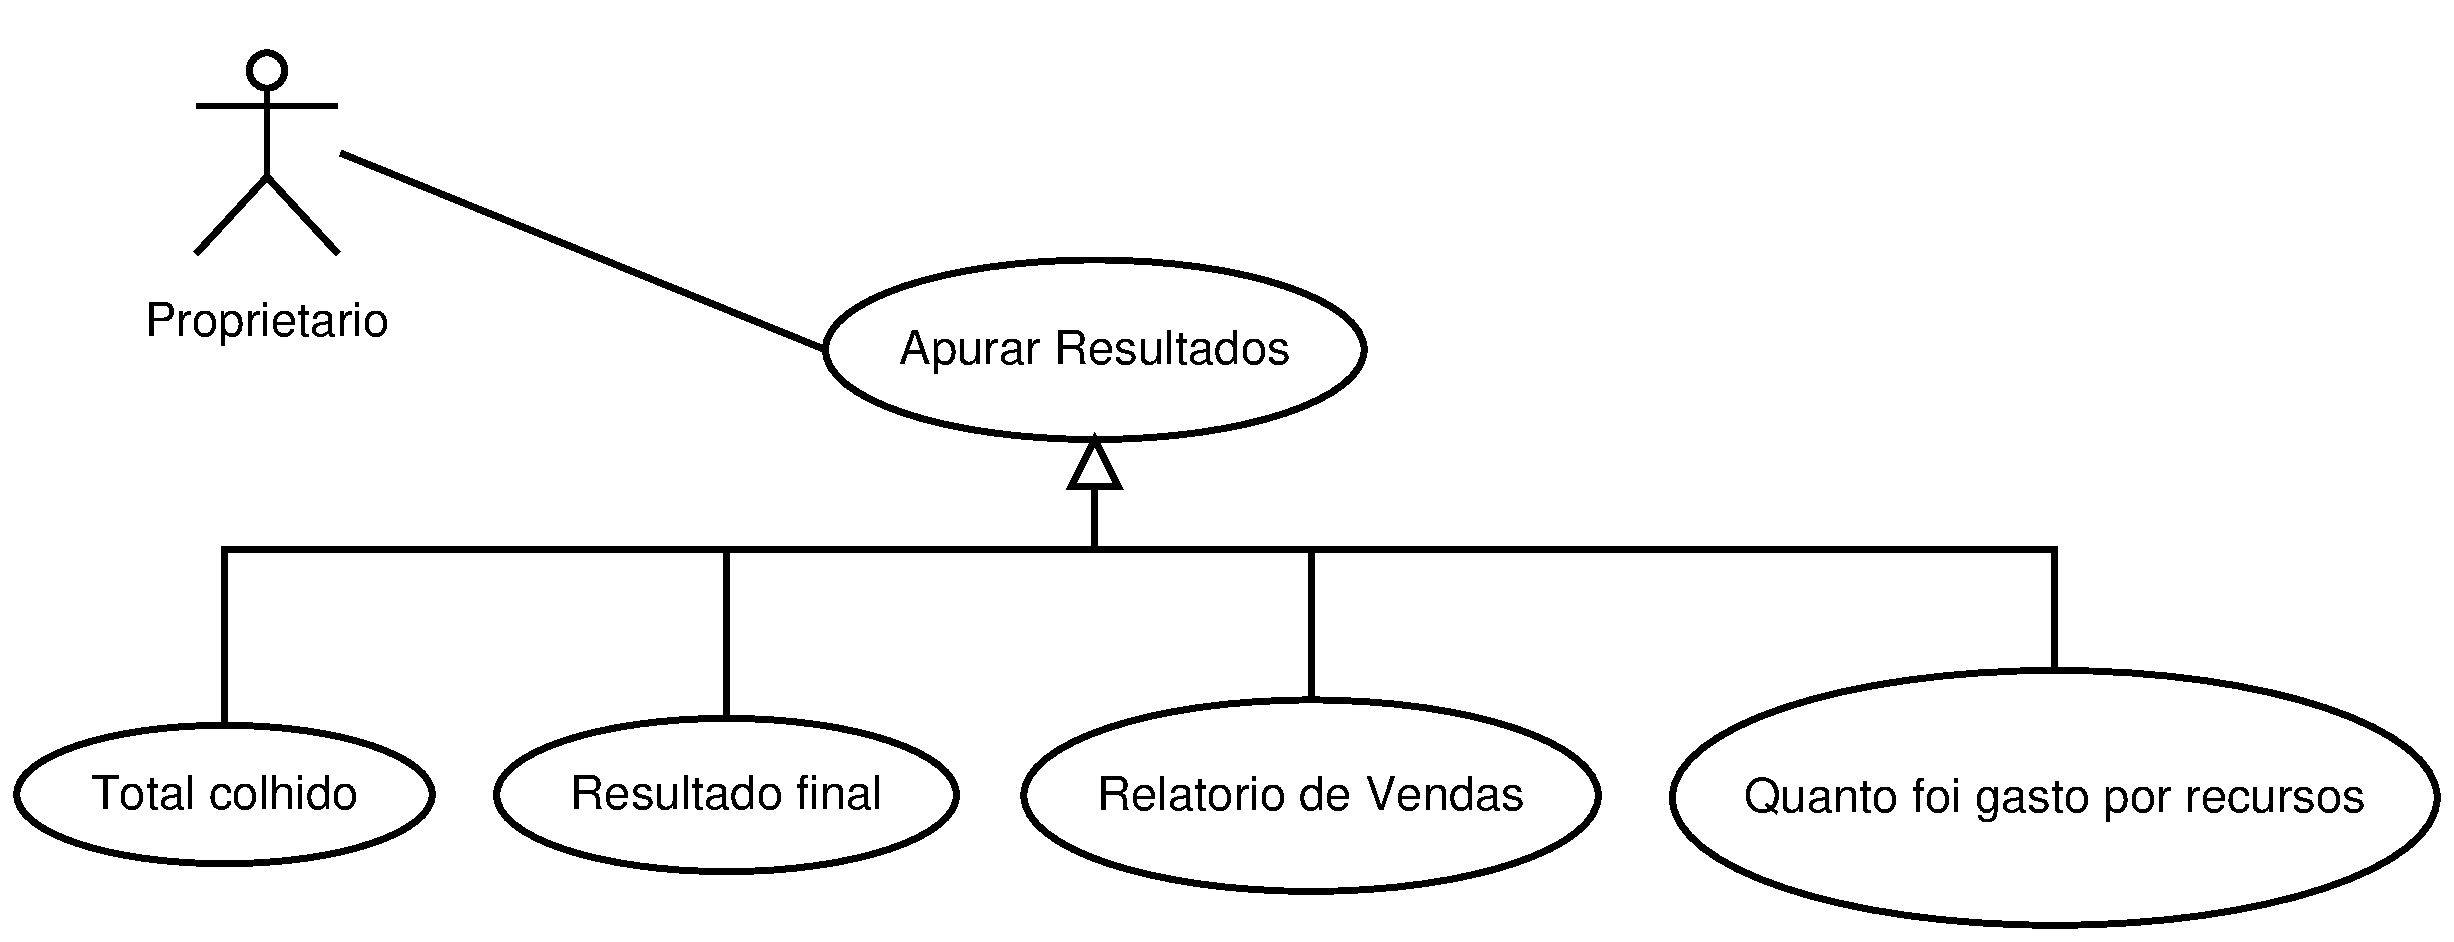
\includegraphics{diagramas/apu_res_caso_uso.eps}} \par}
\caption{Caso de uso de neg�cio ``Apurar resultados''}
\label{fcuar}
\end{figure}

\subsection{Modelagem conceitual}
\paragraph{Por este caso de uso exclusivamente gerar informa��o baseada nos 
dados j� cadastrados no sistema, o modelo conceitual deste caso de uso
� o modelo conceitual da aplica��o.}

\subsection{Projeto navegacional}
\paragraph{O esquema navegacional usado � o mesmo esquema navegacional da
aplica��o.}
\paragraph{O diagrama de contexto est� representado na Figura \ref{fdcar}.}

\begin{figure}[!b]
{\centering \resizebox*{\textwidth}{0.4\textheight}{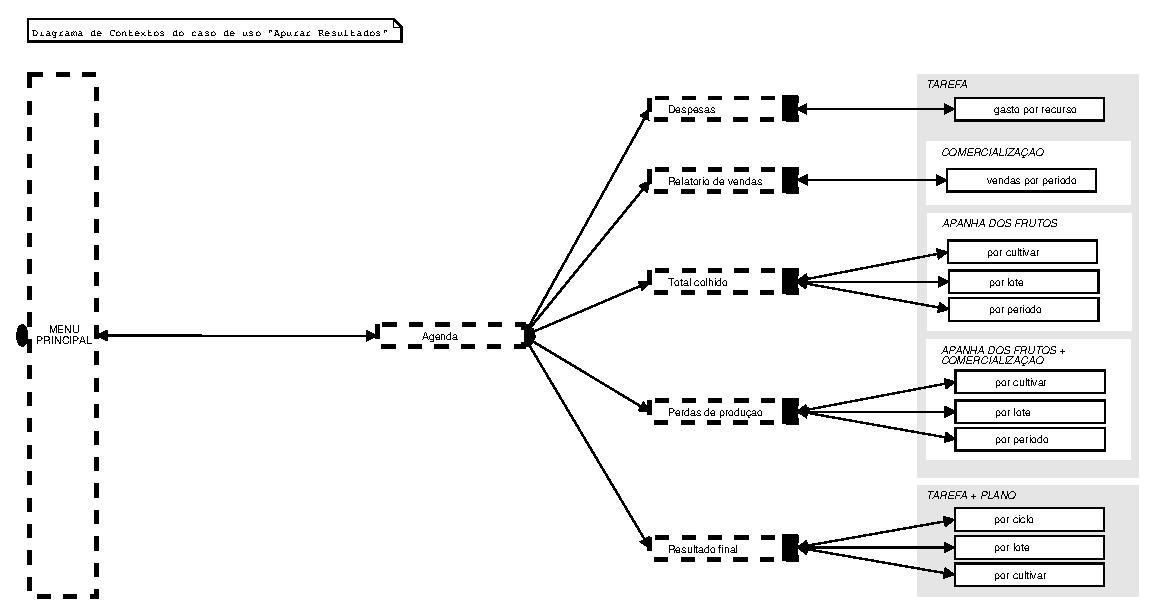
\includegraphics{diagramas/apu_res_diag_contextos.eps}} \par}
\caption{Diagrama de contextos do caso de uso de neg�cio ``Apurar resultados''}
\label{fdcar}
\end{figure}

\subsection{Projeto de interface abstrata}
\paragraph{Os ADVs dos relat�rios deste caso de uso, est�o representados na
Figura \ref{fadvar}.}

\begin{figure}[!b]
{\centering \resizebox*{\textwidth}{0.85\textheight}{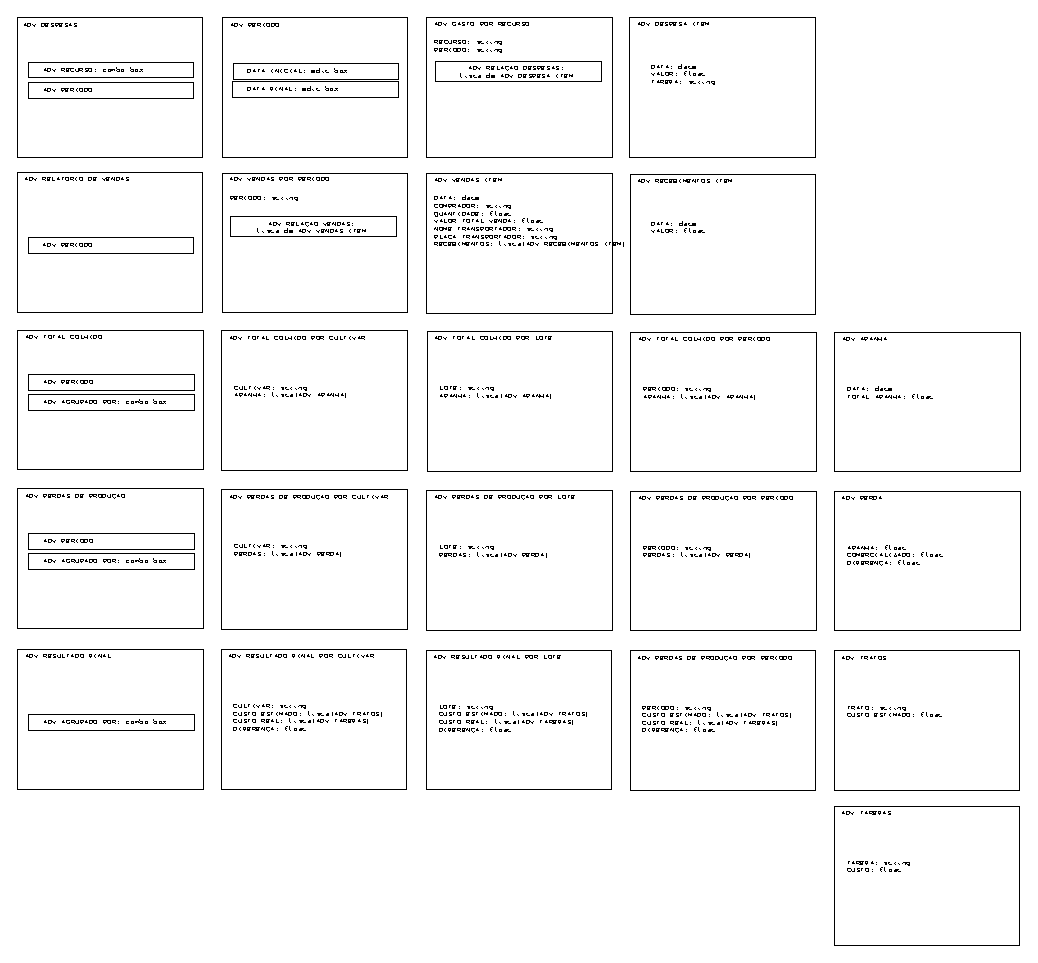
\includegraphics{diagramas/apu_res_adv.eps}} \par}
\caption{ADVs do caso de uso de neg�cio ``Apurar resultados''}
\label{fadvar}
\end{figure}


\chapter{CONCLUS�O}
\paragraph{Considerando que o desenvolvimento deste trabalho come�ou em
Abril do ano de 2000, esta monografia � o resultado de 8 meses de estudo 
em diversas �reas do saber. Essa diversidade de mat�rias estudadas s�
foi poss�vel dado a forma como a disciplina de Projeto de Gradua��o � 
conduzida. Acredito que o grande m�rito desta disciplina seja a possibilidade
do aluno poder escolher o tema do seu projeto, tema esse que deve possuir 
um cunho inovador e foco direcionado para a comunidade local.
Essas duas exig�ncias estabelecem um desafio interessante para a escolha do tema, 
j� que a avalia��o � baseada na capacidade do aluno de desenvolver racioc�nio, 
integrar conceitos adquiridos ao longo do curso e realizar 
contribui��o para ensino, pesquisa e extens�o \cite{cac}.}
\paragraph{Para o desenvolvimento deste trabalho a Internet provou ser 
realmente uma grande biblioteca, basta verificar as refer�ncias bibliogr�ficas
e concluir que 80\% do referencial te�rico utilizado
neste trabalho provem de Universal Resource Locators (URL\footnote{%
\textbf{Universal Resource Locator} � a forma de representa��o para endere�o de 
informa��es na Internet. � disposta na forma 
\emph{servi�o}://\emph{servidor}/\emph{arquivo}. Um exemplo de URL seria
http://projetoacanguacu.yi.org/index.php, onde o servi�o � \emph{http},
o servidor � \emph{projetoacanguacu.yi.org} e o arquivo \emph{index.php}.}). 
Al�m de conte�do est�tico, ainda foi
poss�vel entrar em contato com os autores de v�rios dos artigos utilizados,
para esclarecimento de d�vidas e/ou troca de id�ias, de forma barata e
r�pida. 
Sem essa ferramenta, certamente o desenvolvimento deste trabalho seria bem
mais complicado e incompleto. � interessante ressaltar que o software livre
somente conseguiu atingir o n�vel que est� hoje gra�as a essa forma 
independente, ``indisciplinada'' e sem fronteiras para dissemina��o do
conhecimento humano.}
\paragraph{Quando fui escrever este trabalho surgiu a primeira
dificuldade. Como o pretendido era somente utilizar software livre, que
ferramenta eu iria utilizar para escrever esta monografia? Pesquisei alguns
processadores de texto gr�ficos, mas infelizmente n�o encontrei uma ferramenta 
visual completa que atendesse aos requisitos tipogr�ficos que esta monografia
exige. Foi ent�o que descobri o \LaTeX{} e posso 
dizer que foi ``amor a primeira compila��o''. Como o \LaTeX{} � baseado em classes
de documento e at� ent�o n�o existia uma classe de documento para monografias
da ESIN, resolvi criar uma. N�o sou perito em \LaTeX{}
mas tive que estudar mais profundamente a linguagem para conseguir criar a 
classe que utilizei para escrever o documento que est�s lendo. Disponibilizarei
a classe na Internet para que futuros formandos da ESIN possam usufruir dessa 
facilidade caso prefiram utilizar \LaTeX{} como ferramenta para escritura de 
sua monografia.}
\paragraph{Outra dificuldade encontrada foi a fraca implementa��o do modelo
orientado a objetos nas ferramentas que utilizei na constru��o do prot�tipo
da aplica��o de gest�o para pomar de pessegueiros, principalmente na 
implementa��o do PHP.} 
\paragraph{Possuir um propriet�rio de pomar de pessegueiros em casa � uma
facilidade que merece ser ressaltada. Isso possibilitou uma resposta mais
r�pida e objetiva frente aos questionamentos e demonstra��es que precisei
efetuar.}
\paragraph{Pretendo entrar em contato com �rg�os que lidam com os
produtores de p�ssego, como EMBRAPA e EMATER, procurando buscar uma forma
de viabilizar o di�logo entre estas entidades e os produtores, atrav�s da 
publica��o de informa��es e at� consultas virtuais (lembre-se que a Internet 
possibilita isso).}
\paragraph{Paralelamente a este trabalho, motivado pela filosofia do
software livre e por um grande senso de ``querer fazer as coisas acontecerem''
criei uma proposta para democratiza��o da inform�tica na cidade onde resido,
chamada ``Projeto Acangua�u''. Uma c�pia desta proposta � apresentada no 
ANEXO B.}
\paragraph{Ap�s obter o t�tulo de bacharel em An�lise de Sistemas, 
pretendo finalmente implantar o projeto, disseminando assim
o software livre por lugares que ainda n�o tem id�ia dos benef�cios que a 
filosofia GNU junto da consci�ncia civil dos cidad�os podem proporcionar a 
regi�o onde vivo.}


\chapter{ANEXOS}
\section{ANEXO A}
\verbatiminput{gpl.txt}
\newpage{}
\section{ANEXO B}
\verbatiminput{proposta.txt}


\begin{thebibliography}{bibliografia}

\advance\leftskip by 1.5em

\advance\itemindent by -1.5em

\bibitem[Ald 00]{ALD93}

ALDRICH, Douglas F. Dominando o Mercado Digital. S�o Paulo: Makron Books, 2000.

\bibitem[ALL 00]{alliance}

ALLIANCE website. Dispon�vel por WWW em \url{http://www.allos.org}, [s.d.]. (jun. 2000)

\bibitem[AMA 00]{amaya}

AMAYA website. Dispon�vel por WWW em \url{http://www.w3.org/Amaya/}, [s.d.]. (nov. 2000)

\bibitem[APA 00]{apache}

APACHE Project website. Dispon�vel por WWW em \url{http://www.apache.org}, [s.d.]. (jun. 2000)

\bibitem[APP 00]{appwatch}

APPWATCH.COM website. Dispon�vel por WWW em \url{http://appwatch.zdnet.com}, [s.d.]. (abr. 2000)

\bibitem[ARM 00]{armadillo}

ARMADILLO website. Dispon�vel por WWW em \url{http://www.gzilla.com/index.html}, [s.d.]. (nov. 2000)

\bibitem[Bar s.d.]{BAR s.d.}

BARROS Pablo Fernando do R�go. UML Linguagem de Modelagem Unificada. Aracaju: Universidade Tirantes, [s.d.] 74 p. (Monografia, Centro de Ci�ncias Formais e Tecnol�gicas)

\bibitem[BBC et al. 00]{BBC00}

BROD Cesar Augusto de Azambuja, BUSCH JR. Carlos Alberto, CASTRO Maur�cio de et al. SAGU-FMS - Sistema Aberto de Gest�o Unificada para Escolas de Ensino Fundamental, M�dio e Superior. In: 1� F�RUM INTERNACIONAL SOFTWARE LIVRE 2000, 1, 2000, Porto Alegre. Anais Workshop sobre Software Livre. Porto Alegre: Sociedade Brasileira de Computa��o, 2000. p. 65-68

\bibitem[BCu 89]{BECK89}

BECK, Kent, CUNNINGHAM, Ward. \emph{A laboratory for teaching object-oriented thinking.} Dispon�vel por WWW em \url{http://c2.com/doc/oopsla89/papaer.html}, 1989. (ago. 2000)

\bibitem[Ber 00]{BERARD}

BERARD, Edward V. \emph{What is a methodology?} Dispon�vel por WWW em \url{http://www.toa.com/pub/methodology-article.txt}, [s.d.]. (ago. 2000)

\bibitem[BSc 98]{natacha}

BARROSO, Natacha G�ell, SCHWABE, Daniel. \emph{Projeto de Navega��o em Aplicativos Hiperm�dia Orientado ao Usu�rio.} Dispon�vel por WWW em \url{http://www.telemidia.puc-rio.br/oohdm/Mod_Navegacao.pdf}, 1998. (out. 2000)

\bibitem[BSD 00]{freebsd}

FREEBSD website. Dispon�vel por WWW em \url{http://www.freebsd.org}, [s.d.]. (jun. 2000)

\bibitem[CHI 00]{chimera}

CHIMERA website. Dispon�vel por WWW em \url{http://www.cs.unlv.edu/chimera/}, [s.d.]. (nov. 2000)

\bibitem[Coe 00]{COELHO}

COELHO, Marcelo de Miranda. \emph{O uso de estruturas navegacionais e vistas abstratas de dados no OOHDM e conceitos de objetos multim�dia para a constru��o de uma aplica��o}. Dispon�vel por WWW em \url{http://tathy.comp.ita.cta.br/~coelho/tgonline/cap1&2.htm}, [s.d.]. (ago. 2000)

\bibitem[Cos 99]{cac}

COSTA, Cristiano Andr� da. \emph{Normas para a apresenta��o do Projeto de Gradua��o na Escola de Inform�tica da UCPel}. Pelotas: Educat, 1999. 51 p.

\bibitem[Cou 97]{COUGO}

COUGO, Paulo. Modelagem conceitual e projeto de bancos de dados. Rio de Janeiro: Campus, 1997. 281 p.

\bibitem[Cox 90]{COX1990}

COX, Brad J. \emph{Planning the Software Industrial Revolution}. Dispon�vel por WWW em \url{http://www.virtualschool.edu/cox/CoxPSIR.html}, 1990. (ago. 1999)

\bibitem[CYo 93]{COADYOURDON}

COAD Peter, YOURDON Edward. Projeto baseado em objetos. 4a. ed. Rio de Janeiro: Campus, 1993. 191 p.

\bibitem[CZL 00]{CIOCIOLA}

CIOCIOLA, D�bora, ZAMBALDE, Andr� Luiz, LOPES, Alfredo Scheid. \emph{Desenvolvimento de um aplicativo hiperm�dia para o setor agropecu�rio: OOHDM e autoria toolbook.} Dispon�vel por WWW em \url{http://agrosoft.com/ag97/papers/c4w1730.htm}, [s.d.]. (ago. 2000)

\bibitem[DIA 00]{dia}

DIA website. Dispon�vel por WWW em \url{http://www.lysator.liu.se/~alla/dia/}, [s.d.]. (jun. 2000)

\bibitem[DOS 00]{freedos}

FREEDOS website. Dispon�vel por WWW em \url{http://www.freedos.org}, [s.d.]. (jun. 2000)

\bibitem[EBi 00]{BIBITEX}

ESTILO BibTex com as normas da ABNT. Dispon�vel por WWW em \url{http://www.if.ufrgs.br/hadrons/abnt/abnt.html}, [s.d.]. (set. 2000)

\bibitem[ERO 00]{eros}

EROS website. Dispon�vel por WWW em \url{http://www.eros-os.org}, [s.d.]. (jun. 2000)

\bibitem[Fer 93]{AURELIO}

FERREIRA, Aur�lio Buarque de Holanda. Minidicion�rio da L�ngua Portuguesa. 4a. ed. Rio de Janeiro: Nova Fronteira, 1993. 577 p.

\bibitem[FOS 00]{freeos}

FREEOS website. Dispon�vel por WWW em \url{http://www.freeos.com}, [s.d.]. (abr. 2000)

\bibitem[Fow 00]{TOOAD}

FOWLER, Martin. \emph{Techniques for Object Oriented Analysis and Design}. Dispon�vel por WWW em \url{http://www2.awl.com/cseng/titles/0-201-89542-0/techniques/}, [s.d.] (ago. 2000)

\bibitem[Fow 00a]{umlessencial}

FOWLER, Martin. \emph{UML Essencial}. Porto Alegre: Bookman, 2000. 169p. 

\bibitem[FRE 00]{fresmeat}

FRESHMEAT.NET website. Dispon�vel por WWW em \url{http://freshmeat.net}, [s.d.]. (abr. 2000)

\bibitem[Fur 98]{FURLAN}

FURLAN, Jos� Davi. Modelagem de Objetos atrav�s da UML - The Unified Modeling Language. S�o Paulo: Makron Books, 1998. 325 p.

\bibitem[GAL 00]{galeon}

GALEON website. Dispon�vel por WWW em \url{http://galeon.sourceforge.net/}, [s.d.]. (nov. 2000)

\bibitem[Gas 00]{GASS2000}

GASS, Elvino Bohn. \emph{Software Livre}. 1� ed. Porto Alegre: Corag, 2000. 25 p.

\bibitem[GHJ et al 00]{PADROESPROJETO}

GAMMA, Erich, HELM, Richard, JOHNSON, Ralph, VLISSIDES, John. \emph{Padr�es de Projeto: solu��es reutiliz�veis de software orientado a objetos}. Porto Alegre: Bookman, 2000. 364 p.

\bibitem[GHT 00]{ghttpd}

GHTTPD website. Dispon�vel por WWW em \url{http://www.gaztek.co.uk/ghttpd}, [s.d.]. (jun. 2000)

\bibitem[GJS 00]{GNUJSP}

GNUJSP website. Dispon�vel por WWW em \url{http://www.klomp.org/gnujsp}, [s.d.]. (out. 2000)

\bibitem[GNO 00]{gnome}

GNOME Desktop Environment website. Dispon�vel por WWW em \url{http://www.gnome.org}, [s.d.]. (out. 2000)

\bibitem[GNU 00]{GNU2000}

GNU Project website. Dispon�vel por WWW em \url{http://www.gnu.org}, [s.d.]. (mai. 2000)

\bibitem[HB 00]{hb}

HB Pre-processor website. Dispon�vel por WWW em \url{http://bachue.com/hb/hb.cgi}, [s.d.]. (jun. 2000)

\bibitem[HUR 00]{hurd}

GNU/HURD website. Dispon�vel por WWW em \url{http://www.gnu.ai.mit.edu/software/hurd}, [s.d.]. (jun. 2000)

\bibitem[INT 00]{interbase}

INTERBASE website. Dispon�vel por WWW em \url{http://www.interbase.com}, [s.d.]. (jun. 2000)

\bibitem[JAP 00]{japhar}

JAPHAR website. Dispon�vel por WWW em \url{http://www.japhar.org}, [s.d.]. (out. 2000)

\bibitem[KAF 00]{kaffe}

KAFFE website. Dispon�vel por WWW em \url{http://www.kaffe.org}, [s.d.]. (out. 2000)

\bibitem[KDE 00]{kde}

K Desktop Environment website. Dispon�vel por WWW em \url{http://www.kde.org}, [s.d.]. (out. 2000)

\bibitem[Ken 89]{KENT}

KENT, Beck. A Laboratory For Teaching Object-Oriented Thinking. Dispon�vel por WWW em \url{http://c2.com/doc/oopsla89/paper.html}, 1989. (ago. 1999)

\bibitem[KON 00]{konqueror}

KONQUEROR website. Dispon�vel por WWW em \url{http://www.konqueror.org}, [s.d.]. (nov. 2000)

\bibitem[LAG 00]{lago}

LAGO website. Dispon�vel por WWW em \url{http://lago.sourceforge.net}, [s.d.]. (jun. 2000)

\bibitem[LAl 97]{LOBATO}

LOBATO Daniel Corr�a, ALVES Ronnie Cley de Oliveira. An�lise e Projeto de Sistemas M�todo Shlaer-Mellor para OOA e OOD. Bel�m: Universidade Federal do Par�, 1997. 19 p. (Disserta��o, Curso de Especializa��o em An�lise de Sistemas)

\bibitem[LEA 00]{leap}

LEAP website. Dispon�vel por WWW em \url{http://leap.sourceforge.net}, [s.d.]. (jun. 2000)

\bibitem[LNX 00]{linux}

LINUX website. Dispon�vel por WWW em \url{http://www.linux.org}, [s.d.]. (jun. 2000)

\bibitem[Loh 96]{LOH}

LOH, Stanley. Ambientes de desenvolvimento de software e ferramentas CASE. [s.l.]: Universidade Cat�lica de Pelotas, 1996. 27 p. 

\bibitem[MID 00]{midgard}

MIDGARD project website. Dispon�vel por WWW em \url{http://www.midgard-project.org}, [s.d.]. (jun. 2000)

\bibitem[MNX 00]{minix}

MINIX website. Dispon�vel por WWW em \url{http://www.cs.vu.nl/~ast/minix.html}, [s.d.]. (jun. 2000)

\bibitem[MOM 00]{livropgsql}

MOMJIAM, Bruce. \emph{PostgreSQL Introduction and Concepts}. Dispon�vel por WWW em \url{http://www.postgresql.org/docs/aw_pgsql_book/aw_pgsql_book.pdf}, [s.d.]. (out. 2000)

\bibitem[MOU 98]{isabela}

MOURA, Isabela. \emph{Um Ambiente para o Suporte ao Projeto e Implementa��o de Sistemas de Informa��o Baseados na WWW}. Dispon�vel por WWW em \url{http://www.telemidia.puc-rio.br/oohdm/oohdmweb/docs/TeseIsabela.zip}, 1998. (out. 2000)

\bibitem[MOZ 00]{mozilla}

MOZILLA website. Dispon�vel por WWW em \url{http://www.mozilla.org}, [s.d.]. (nov. 2000)

\bibitem[MRa 98]{PESSEGUEIRO}

MEDEIROS, Carlos Alberto Barbosa, RASEIRA, Maria do Carmo Bassols. \emph{A cultura do Pessegueiro}. Pelotas: Embrapa-CPACT, 1998. 350p.

\bibitem[MYS 00]{mysql}

MYSQL website. Dispon�vel por WWW em \url{http://www.mysql.com}, [s.d.]. (jun. 2000)

\bibitem[NET 00]{netbsd}

NETBSD website. Dispon�vel por WWW em \url{http://www.netbsd.org}, [s.d.]. (jun. 2000)

\bibitem[OPE 00]{openbsd}

OPENBSD website. Dispon�vel por WWW em \url{http://www.openbsd.org}, [s.d.]. (jun. 2000)

\bibitem[PCD et al 00]{DINHEIROPARAQUEMPRECISA}

PARERA Ant�nio Jo�o, COPPETTI Clarice, DUTRA Claudio et al. DINHEIRO PARA QUEM PRECISA; Alguns motivos para o Projeto Software Livre do Rio Grande do Sul. In: 1� F�RUM INTERNACIONAL SOFTWARE LIVRE 2000, 1, 2000, Porto Alegre.Anais Workshop sobre Software Livre... Porto Alegre: Sociedade Brasileiro de Computa��o, 2000. p. 9-13

\bibitem[PGS 00]{pgsql}

POSTGRESQL website. Dispon�vel por WWW em \url{http://www.postgresql.org}, [s.d.]. (jun. 2000)

\bibitem[PHP 00]{php}

PHP website. Dispon�vel por WWW em \url{http://php.net}, [s.d.]. (jun. 2000)

\bibitem[Piz 98]{pizzol}

PIZZOL, Andr�a Miranda. \emph{Um Framework para Implementa��o na WWW de Aplica��es Hiperm�dia Modeladas com OOHDM}. Dispon�vel por FTP an�nimo em webengs.lmf-di.puc-rio.br, no arquivo /oohdm/oohdmjava/tese.zip, 1998. (out. 2000)

\bibitem[POL 00]{polyjsp}

PolyJSP website. Dispon�vel por WWW em \url{http://www.plenix.org/polyjsp/}, [s.d.]. (out. 2000)

\bibitem[RAT 97]{UMLNOTATION}

RATIONAL SOFTWARE CORPORATION. \emph{UML Notation Guide version 1.1}. Dispon�vel por WWW em \url{http://www.platinum.com/corp/uml/nota_11.pdf}, 1997. (set. 2000)

\bibitem[RAT 97a]{UMLSUMMARY}

RATIONAL SOFTWARE CORPORATION.\emph{ UML Summary version 1.1}. Dispon�vel por WWW em \url{http://www.platinum.com/corp/uml/summ_11.pdf}, 1997. (set. 2000)

\bibitem[RED 00]{redhat}

REDHAT Linux Distribuition Website. Dispon�vel por WWW em \url{http://www.redhat.com}, [s.d.]. (out. 2000)

\bibitem[RES 00]{resin}

RESIN website. Dispon�vel por WWW em \url{http://www.caucho.com/products/resin}, [s.d.]. (out. 2000)

\bibitem[RLS 00]{PFECA}

ROSSI, Gustavo, LYARDET, Fernando, SCHWABE, Daniel. \emph{Patterns for E-commerce applications}. Dispon�vel por WWW em \url{http://www.inf.puc-rio.br/~schwabe/papers/Europlop00.pdf}, 2000. (ago. 2000).

\bibitem[Ros 96]{ROS96}

ROSSI, Gustavo. \emph{Um M�todo Orientado a Objetos para o Projeto de Aplica��es Hiperm�dia.}. Dispon�vel por WWW em \url{http://www-di.inf.puc-rio.br/~schwabe/Tese_Rossi/}, 1996. (ago. 2000).

\bibitem[RSL et al 95]{IWHD}

ROSSI, Gustavo, SCHWABE, Daniel, LUCENA, C.J.P., COWAN, D.D. \emph{An Object-Oriented Model for Designing the Human-Computer Interface Of Hypermedia Applications.} Dispon�vel por FTP an�nimo em \url{ftp.inf.puc-rio.br}, no arquivo \url{/pub/docs/techreports/95_07_rossi.ps.gz}, 1995. (out. 2000)

\bibitem[RSL 99]{WAMAMTCM}

ROSSI, Gustavo, SCHWABE, Daniel, LYARDET, Fernando. \emph{Web Application Models are more than Conceptual Models}. Dispon�vel por WWW em \url{http://www.inf.puc-rio.br/~schwabe/papers/WWWCM99.pdf}, 1999. (set. 2000)

\bibitem[RSL 00]{ARMWAM}

ROSSI, Gustavo, SCHWABE, Daniel, LYARDET, Fernando. \emph{Abstraction and Reuse Mechanisms in Web Application Models}. Dispon�vel por WWW em \url{http://www.inf.puc-rio.br/~schwabe/papers/WWWCM002Expanded.pdf}, 2000. (ago. 2000).

\bibitem[Sch 91]{OOPROJMAN}

SCHULTZ, Ronald. OO project management. Dispon�vel por WWW em \url{http://www.cs.ncl.ac.uk/people/chris.holt/home.formal/workroom/library/OO.project.management.htm}, 1991. (ago. 1999)

\bibitem[Sch 99]{ACUCAMWIS}

SCHARL, Arno. \emph{A Conceptual, User-Centric Approach to Modeling Web Information Systems}. Dispon�vel por WWW em \url{http://ausweb.scu.edu.au/aw99/papers/scharl/paper.html}, 1999. (ago. 2000)

\bibitem[Sch 99]{JUSTADDWATER}

SCHWABE, Daniel. \emph{``Just add Water'' Applications: Hypermedia Application Frameworks}. Dispon�vel por WWW em \url{http://www.inf.puc-rio.br/~schwabe/papers/SchwabeHT99Workshop.pdf}, 1999. (ago. 2000)

\bibitem[SGu 00]{projnav}

SCHWABE, Daniel, GU\"{E}LL, Natacha. \emph{Projeto de Navega��o, baseado em cen�rios, use cases e diagramas de intera��o do usu�rio (UIDs)}. Dispon�vel por WWW em \url{http://www.telemidia.puc-rio.br/oohdm/Mod_Navegacao.pdf}, [s.d.]. (out. 2000)

\bibitem[SK8 00]{skatebrowser}

SKATEBROWSER website. Dispon�vel por WWW em \url{http://freshmeat.net/projects/skatebrowser/homepage/}, [s.d.]. (nov. 2000)

\bibitem[SPo 98]{oohdmweb}

SCHWABE, Daniel, PONTES, Rita de Almeida. \emph{OOHDM-WEB: Rapid Prototyping of Hypermedia Applications in the WWW}. Dispon�vel por WWW em \url{http://www-di.inf.puc-rio.br/~schwabe/papers/MCC-08-98.pdf.gz}, 1998. (out. 2000)

\bibitem[SRE et al. 00]{WDF}

SCHWABE, Daniel, ROSSI, Gustavo, ESMERALDO, Luiselena et al. \emph{Web Design Frameworks: An approach to improve reuse in Web applications.} Dispon�vel por WWW em \url{http://www.inf.puc-rio.br/~schwabe/papers/WWW9WebEngineering.pdf}, [s.d.]. (set. 2000)

\bibitem[SRo 98]{DHAUO}

SCHWABE, Daniel, ROSSI, Gustavo. \emph{Developing Hypermedia Applications using OOHDM}. Dispon�vel por WWW em \url{http://www.inf.puc-rio.br/~schwabe/papers/ExOOHDM.pdf.gz}, 1998. (ago. 2000).

\bibitem[Sey 00]{CLIENTESCOM}

SEYBOLD, Patricia B. CLIENTES.COM. S�o Paulo: Makron Books, 2000. 

\bibitem[SOF 00]{PROJLEI}

SOFTWARE LIVRE - PROJETO DE LEI No. 59/2000 DEPUTADO ELVINO BOHN BASS - PT. Porto Alegre: [s.n.], Mai. 2000.

\bibitem[SQL 00]{sqlserver}

GNU SQL Server website. Dispon�vel por WWW em \url{http://www.ispras.ru/~gsql}, [s.d.]. (jun. 2000)

\bibitem[Sun 00]{jspisthebestone}

SUN Microsystems Inc. \emph{Java Servlet and JavaServer Pages Technology: Comparing Methods for Server Side Dynamic Content}. Dispon�vel por WWW \url{http://javasoft.com/products/jsp/pdf/jspservlet.pdf}, 2000. (out. 2000)

\bibitem[SVi 99]{patricia}

SCHWABE, Daniel, VILAIN, Patr�cia. \emph{Nota��o da Metodologia OOHDM vers�o 1.1}. Dispon�vel por WWW em \url{http://www.telemidia.puc-rio.br/oohdm/notacao_OOHDM_UML.zip}, 1999. (out. 2000)

\bibitem[THT 00]{thttpd}

THTTPD website. Dispon�vel por WWW em \url{http://www.acme.com/software/thttpd}, [s.d.]. (jun. 2000)

\bibitem[TOM 00]{tomcat}

TOMCAT-JAKARTA website. Dispon�vel por WWW em \url{http://jakarta.apache.org/tomcat/index.html}, [s.d.]. (out. 2000)

\bibitem[Ven 99]{VENETIANER}

VENETIANER, Tom. Como Vender seu Peixe na Internet. Rio de Janeiro: Campus, 1999.

\bibitem[VSS 00]{UID}

VILAIN, Patr�cia, SCHWABE, Daniel, SOUZA, Clarisse Sieckenius de. \emph{A Diagrammatic Tool for Representing User Interaction in UML}. Dispon�vel por WWW em \url{http://www.inf.puc-rio.br/~schwabe/papers/UML2000.pdf}, 2000. (agosto 2000).

\bibitem[XIT 00]{xitami}

XITAMI website. Dispon�vel por WWW em \url{http://www.xitami.com}, [s.d.]. (jun. 2000)

\bibitem[ZOP 00]{zope}

ZOPE website. Dispon�vel por WWW em \url{http://www.zope.org}, [s.d.]. (jun. 2000)

\end{thebibliography}


\end{document}
